% INSLIB -- Software Architecture and Mathematical Models
%
% Build: make (in this directory, uses latexmk/pdflatex)
%
% Scope: architecture, design decisions and the mathematical models of
% the INSLIB library. The requirements themselves live in
% ../requirements/ (machine-checked database), this document only
% references that process, it does not duplicate it.
%
% Matrices: uppercase bold letter \mathbf{R}
% 1x1 Matrices: italic uppercase letter
% Vector: lowercase \vec{v}
% Scalar: lowercase
% Quaternion: \mathbf{q}
% Frame transformation from b to n: \mathbf{q}^n_b

\documentclass[11pt,a4paper]{article}

\usepackage[T1]{fontenc}
\usepackage[utf8]{inputenc}
\usepackage{lmodern}
\usepackage{microtype}
\usepackage[margin=2.6cm]{geometry}
\usepackage{amsmath,amssymb,bm}
\usepackage{booktabs}
\usepackage{array}
\usepackage{multirow}
\usepackage{longtable}
\usepackage{pdflscape} % rotates just the config.yaml <-> C API table's pages
\usepackage{siunitx}
\usepackage{graphicx}
\usepackage{tikz}
\usetikzlibrary{positioning,arrows.meta,fit,backgrounds,calc}
\usepackage[colorlinks=true,linkcolor=blue!50!black,citecolor=blue!50!black,urlcolor=blue!50!black]{hyperref}

% --- Notation macros ---------------------------------------------------------
\newcommand{\vect}[1]{\bm{#1}}
\newcommand{\mat}[1]{\bm{#1}}
\newcommand{\T}{^{\mathsf{T}}}
\newcommand{\cross}[1]{\left[#1\right]_{\times}}   % skew-symmetric matrix
\newcommand{\nframe}{n}
\newcommand{\bframe}{b}
\newcommand{\eframe}{e}
\newcommand{\Rbn}{\mat{R}_{\bframe}^{\nframe}}
\newcommand{\Rne}{\mat{R}_{\nframe}^{\eframe}}
\newcommand{\qbn}{\vect{q}_{\bframe}^{\nframe}}
\newcommand{\dt}{\Delta t}
\newcommand{\diag}{\operatorname{diag}}
\newcommand{\code}[1]{\texttt{#1}}

% --- YAML syntax highlighting for config.yaml listings -----------------------
% (xcolor comes in via tikz, listings needs no shell-escape, unlike minted)
\usepackage{listings}
\definecolor{cfgKey}{RGB}{28,78,158}       % keys / section names
\definecolor{cfgComment}{RGB}{110,110,110} % # comments
\definecolor{cfgString}{RGB}{34,110,54}    % quoted strings / enum values
\lstdefinelanguage{inslibyaml}{
  % every recognised config.yaml key + the enum values, coloured as keywords
  morekeywords={name,aiding,init,automotive_mode,automotive_min_speed_mps,
    automotive_min_yaw_stddev_deg,chi2_disable,chi2_reject_alpha,
    allow_unlimited_deadreckoning,max_deadreckoning_sec,baro_height_disable,
    gyro_bias_window_sec,auto_init_window_sec,
    imu,gnss,init_stddev,init_hint,mag,baro,ahrs,score,origin,crazyflie,
    free_inertial_start,
    lim_groves_pos_rms_factor,
    gyr_psd,acc_psd,gyr_bias_rw,acc_bias_rw,gyr_fixed_bias,acc_fixed_bias,
    gyr_misalignment,acc_misalignment,zero_vel_stddev_mps,
    zero_rot_stddev_deg,auto_zupt_static_gyr_deg,auto_zupt_static_acc_mps2,
    auto_zupt_max_vel_mps,
    auto_zupt_max_vel_stddev_mps,auto_zupt_static_gyr_stddev_deg,
    auto_zupt_static_acc_stddev_mps2,auto_zupt_dwell_sec,
    auto_zupt_min_interval_sec,auto_zupt_disable,
    auto_zupt_velocity_blind_disable,
    pos_pred_stddev_m_sqrts,vel_pred_stddev_mps_sqrts,
    rpy_pred_stddev_rad_sqrts,leverarm_frd,delay_ms,
    max_horizontal_pos_stddev_m,max_vertical_pos_stddev_m,
    max_horizontal_vel_stddev_mps,max_vertical_vel_stddev_mps,
    start_max_horizontal_pos_stddev_m,start_max_vertical_pos_stddev_m,
    start_max_horizontal_vel_stddev_mps,start_max_vertical_vel_stddev_mps,
    stop_max_horizontal_pos_stddev_m,stop_max_vertical_pos_stddev_m,
    stop_max_horizontal_vel_stddev_mps,stop_max_vertical_vel_stddev_mps,
    init_dwell_sec,init_dwell_disable,stop_dwell_sec,stop_disable,pos_decimation,min_delay_ms,
    pos_stddev_fallback_m,vel_stddev_fallback_mps,pos_cov_scale,pos_cov_scale_height,vel_cov_scale,
    pos_stddev_floor_hor_m,pos_stddev_floor_ver_m,vel_stddev_floor_hor_mps,
    vel_stddev_floor_ver_mps,
    pos_stddev_cap_hor_m,pos_stddev_cap_ver_m,vel_stddev_cap_hor_mps,
    vel_stddev_cap_ver_mps,acc_envelope_tau_sec,
    vel_noise_acc_scale_hor,vel_noise_acc_scale_ver,vel_noise_acc_window_sec,
    pos_init_stddev_m,vel_init_stddev_mps,rpy_init_stddev_rad_deg,
    yaw_init_stddev_rad_deg,acc_bias_init_stddev_mps2,gyr_bias_init_stddev_rps_deg,
    roll_deg,pitch_deg,rpy_stddev_deg,yaw_deg,yaw_stddev_deg,
    enable,stddev_ut,min_delay_ms,wmm_year,estimate_bias,fixed_bias,misalignment,stddev_m,acc_bias_rw,
    h_process_noise,acc_bias_init_mps2,acc_noise_mps2_sqrthz,gyr_noise_psd,acc_noise_mps2,
    local_gnss_rw_stddev_mps,local_gnss_chi2_threshold,
    local_gnss_min_update_interval_sec,local_gnss_stddev_inflation_factor,
    warmup_sec,min_epochs,ahrs,attitude,lim_pos_rms_m,lim_att_bias_deg,lim_att_std_deg,
    lim_yaw_bias_deg,lim_yaw_std_deg,
    lim_baro_rms_m,lim_baro_bias_m,lim_baro_max_m,
    lim_ellipsoid_rms_m,lim_ellipsoid_bias_m,lim_ellipsoid_max_m,
    lim_ars_att_bias_deg,lim_ars_roll_std_deg,lim_ars_pitch_std_deg,
    lim_ars_yaw_drift_deg_min,inputs},
  otherkeywords={gnss,ref,none,auto,true,false},
  keywordstyle=\color{cfgKey},
  comment=[l]{\#},
  commentstyle=\color{cfgComment}\itshape,
  morestring=[b]",
  morestring=[b]',
  stringstyle=\color{cfgString},
  sensitive=true,
}
\lstdefinestyle{cfg}{
  language=inslibyaml,
  basicstyle=\ttfamily\footnotesize,
  columns=fixed,
  keepspaces=true,
  showstringspaces=false,
  frame=none,
  aboveskip=0.7em, belowskip=0.4em,
}

\title{\textbf{INSLIB}\\[2mm]
       \large Software Documentation and Mathematical Models\\[1cm]
       
\includegraphics[width=0.33\textwidth]{figures/inslib_logo.pdf}
}
\author{Jan Zwiener \\ \texttt{jan@zwiener.org}}
\date{\today}

\begin{document}
\maketitle

\begin{abstract}
\noindent
INSLIB is a portable C-only (C11) library for 3D navigation state estimation.
Its core is a 15-state (optionally 18-state) error-state Kalman filter
fusing inertial measurements with (delayed) GNSS position/velocity,
barometer, magnetometer, local position references, absolute yaw
references, scalar ground speed and zero-velocity / zero-rotation
information. Around it the library provides two standalone attitude filters
(ARS/AHRS), a baro/accelerometer vertical channel filter
(\code{baro\_\allowbreak{}alt}), a local-height-to-ellipsoid offset filter, a World
Magnetic Model (WMM) lookup and a wrapper (\code{nav\_\allowbreak{}suite}) that runs all
filters in parallel with graceful degradation. All covariances are
maintained in UDU (``square-root'') factorisation (Bierman/Thornton).  The
code uses no heap and no OS services, and its per-epoch execution time is
bounded by design. This document describes the software architecture, the
design decisions and the mathematical models implemented.
\end{abstract}

\tableofcontents
\clearpage

% ==============================================================================
\section{Introduction}
% ==============================================================================

\subsection{Scope and goals}

INSLIB targets embedded navigation applications (vehicles, aircraft,
robots, indoor platforms) with aerospace-style engineering constraints:

\begin{itemize}
  \item \textbf{Portable C11.} No OS dependencies, no compiler
        extensions.
  \item \textbf{No heap/dynamic memory.} All state lives in caller-provided structs,
        the library never calls \code{malloc}/\code{free}.
  \item \textbf{Bounded execution time (WCET).} No unbounded
        loops, recursion, or input-dependent iteration counts in the
        per-epoch path.
  \item \textbf{Single-precision hot path.} Strapdown, prediction and
        fusion run in 32-bit IEEE 754 \code{float}. 64-bit \code{double} is confined to the
        absolute-position anchor (ECEF origin, latitude/longitude/height
        bookkeeping), touched only at initialisation, once per GNSS
        epoch and in accessors.
  \item \textbf{Fail-operational robustness.} Non-finite inputs (NaN, Inf) are
        dropped at the API boundary, implausible measurements are
        statistically screened, and rejections are counted
        in diagnostics.
\end{itemize}

Development follows a requirements-first workflow: behaviour is captured in a
machine-checked requirements database (\code{requirements/}, checked by
\code{make reqs}) and verified by unit/integration tests (\code{make test}) and
replays of real datasets (\code{make datasets}). This document does not restate
the requirements, it explains the architecture, the mathematics, and the tuning
parameters.

\subsection{Module overview}

\begin{center}
\small
\begin{tabular}{@{}lp{4.1cm}p{6.9cm}@{}}
\toprule
\textbf{Module} & \textbf{Files} & \textbf{Purpose} \\
\midrule
INS      & \code{ins.[ch]}       & 15/18-state Error-State Kalman Filter: position, velocity, attitude, IMU biases, optional magnetometer hard-iron bias. \\
ahrs       & \code{ahrs.[ch]}        & Standalone 5/6-state attitude filter (ARS: roll/pitch, AHRS: roll/pitch/yaw with magnetometer heading). \\
baro\_alt  & \code{baro\_\allowbreak{}alt.[ch]}   & 3-state baro/accelerometer vertical channel filter, plus \code{local\_\allowbreak{}gnss\_\allowbreak{}alt\_\allowbreak{}t}, a 1-state local-height-to-ellipsoid offset filter. \\
nav\_suite & \code{nav\_\allowbreak{}suite.[ch]}  & Wrapper: runs INS + two AHRS instances + vertical filters in parallel, mode arbitration, vertical datum alignment, best-source accessors. \\
geodetic\_toolbox & \code{geodetic\_\allowbreak{}toolbox.[ch]} & Quaternion algebra, WGS84 geodesy, gravity model, Earth/transport rate. Reusable outside INSLIB. \\
magnetic\_model & \code{magnetic\_\allowbreak{}model.[ch]}, \code{wmm\_\allowbreak{}lut.h} & World Magnetic Model lookup (declination, inclination, field strength, NED reference vector) from a generated grid. Reusable. \\
sensor\_defaults & \code{sensor\_\allowbreak{}defaults.h} & Shared consumer-MEMS gyro noise defaults for INS and AHRS (see \S\ref{sec:defaults}). \\
KFCore     & submodule               & \code{linalg} (column-major matrix functions), \code{kalman\_\allowbreak{}udu} (Bierman/Thornton UDU routines). \\
\bottomrule
\end{tabular}
\end{center}

% ==============================================================================
\section{Conventions and notation}
% ==============================================================================
\label{sec:conventions}

\begin{itemize}
  \item \textbf{Body frame ($\bframe$):} FRD -- $x$ forward, $y$ right,
        $z$ down, right-handed.
  \item \textbf{Navigation frame ($\nframe$):} NED -- north, east, down,
        local-level frame.
  \item \textbf{Earth frame ($\eframe$):} ECEF (WGS84).
  \item \textbf{Attitude:} Hamilton quaternion $\qbn$ with the scalar
        part first ($q_0 = w$), representing the body-to-NED rotation
        $\Rbn$. Euler angles are Tait--Bryan ZYX (roll $\phi$, pitch
        $\theta$, yaw $\psi$).
  \item \textbf{Matrices} are stored column-major (BLAS/LAPACK convention).
  \item \textbf{Timestamps} are \code{int64} microseconds, monotonic.
  \item $\cross{\vect{a}}$ denotes the skew-symmetric cross-product
        matrix, $\cross{\vect{a}}\vect{b} = \vect{a}\times\vect{b}$.
  \item $\vect{f}^\bframe$ is the accelerometer-measured specific force,
        $\vect{\omega}^\bframe_{ib}$ the gyroscope-measured angular
        rate, $\vect{g}^\nframe$ the local gravity (including the
        centrifugal term), $\vect{m}^\nframe$ the magnetic reference
        field.
\end{itemize}

Units are SI throughout: \si{\metre}, \si{\metre\per\second},
\si{\radian}, \si{\radian\per\second}, \si{\metre\per\second\squared},
\si{\pascal}, magnetometer quantities in \si{\micro\tesla} (matching the
World Magnetic Model).

% ==============================================================================
\section{Software architecture}
% ==============================================================================

\subsection{Structure}

Figure~\ref{fig:arch} shows the module dependency structure. The three
estimation modules (INS, AHRS, baro\_alt) are independent of each
other, each can be used standalone. They share only the math layer
(geodetic\_toolbox, magnetic\_model, KFCore) and, for INS/AHRS, the
IMU noise fallback constants (sensor\_defaults.h). The
\code{nav\_\allowbreak{}suite} wrapper is the only module that knows all filters.

\begin{figure}[htbp]
\centering
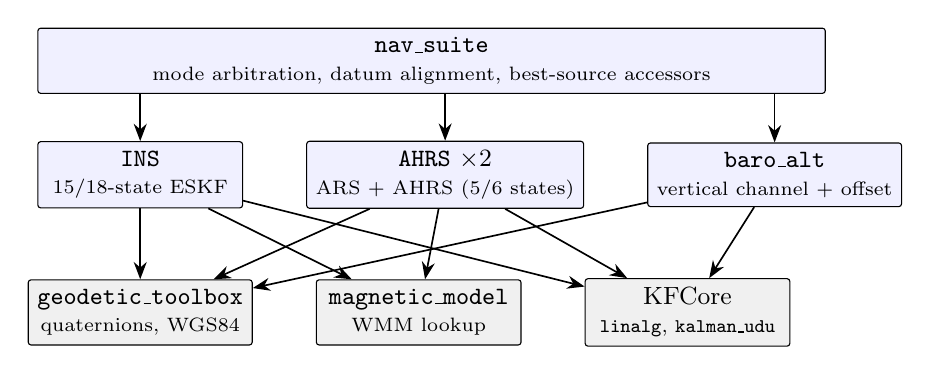
\begin{tikzpicture}[
  node distance=6mm and 8mm,
  box/.style={draw, rounded corners=1pt, fill=blue!6, minimum height=8mm,
              minimum width=26mm, align=center, font=\small},
  lib/.style={box, fill=gray!12},
  arr/.style={-{Stealth[length=2.2mm]}, semithick}
]
  \node[box, minimum width=100mm] (suite) {\code{nav\_\allowbreak{}suite}\\[-1pt]
    {\scriptsize mode arbitration, datum alignment, best-source accessors}};

  \node[box, below=of suite.south west, anchor=north west] (ins)
    {\code{INS}\\[-1pt]{\scriptsize 15/18-state ESKF}};
  \node[box, right=of ins] (ahrs)
    {\code{AHRS} $\times 2$\\[-1pt]{\scriptsize ARS + AHRS (5/6 states)}};
  \node[box, right=of ahrs] (baro)
    {\code{baro\_\allowbreak{}alt}\\[-1pt]{\scriptsize vertical channel + offset}};

  \node[lib, below=9mm of ins] (geo)
    {\code{geodetic\_\allowbreak{}toolbox}\\[-1pt]{\scriptsize quaternions, WGS84}};
  \node[lib, right=of geo] (wmm)
    {\code{magnetic\_\allowbreak{}model}\\[-1pt]{\scriptsize WMM lookup}};
  \node[lib, right=of wmm] (kfcore)
    {KFCore\\[-1pt]{\scriptsize \code{linalg}, \code{kalman\_\allowbreak{}udu}}};

  \draw[arr] (suite.south -| ins) -- (ins);
  \draw[arr] (suite.south -| ahrs)  -- (ahrs);
  \draw[arr] (suite.south -| baro)  -- (baro);

  \draw[arr] (ins) -- (geo);
  \draw[arr] (ins) -- (wmm);
  \draw[arr] (ins) -- (kfcore);
  \draw[arr] (ahrs)  -- (geo);
  \draw[arr] (ahrs)  -- (wmm);
  \draw[arr] (ahrs)  -- (kfcore);
  \draw[arr] (baro)  -- (geo);
  \draw[arr] (baro)  -- (kfcore);
\end{tikzpicture}
    \caption{Module dependencies. Grey modules are (reusable) helper modules:
    \code{geodetic\_\allowbreak{}toolbox}, \code{KFCore}, and \code{magnetic\_\allowbreak{}model} are
    deliberately reusable outside this repository.}
\label{fig:arch}
\end{figure}

\subsection{Data flow: one measurement epoch}

All measurements of one epoch are collected in a single
\code{ins\_\allowbreak{}measurements\_\allowbreak{}t} bundle (every field optional, marked by an
\code{is\_\allowbreak{}valid} flag) and pushed to \code{nav\_\allowbreak{}suite\_\allowbreak{}update}
(or \code{ins\_\allowbreak{}update} when using the core filter alone). Inside
\code{ins\_\allowbreak{}update} the processing order is fixed:

\begin{enumerate}
  \item \textbf{Input sanitisation:} every consumed field is checked for
        NaN/Inf before any arithmetic (\S\ref{sec:robust}).
  \item \textbf{Time-jump handling:} backward steps and oversized
        forward gaps are classified and handled (drop / reset / skip),
        a backward step that \emph{persists} is read as a restarted
        timestamp source (\S\ref{sec:robust}).
  \item \textbf{Strapdown integration} of the nominal state at IMU rate
        (\S\ref{sec:strapdown}).
  \item \textbf{Covariance prediction}, throttled to the configured
        Kalman period rather than the IMU rate (\S\ref{sec:predict}).
  \item \textbf{Measurement fusion} in fixed order: magnetometer,
        absolute yaw, zero-velocity, zero-rotation, local position,
        GNSS position/velocity, barometric height, absolute speed,
        GNSS course-over-ground yaw.
  \item \textbf{History snapshot} into a ring buffer (for delayed
        measurements, \S\ref{sec:delayed}) and \textbf{health check}.
\end{enumerate}

The wrapper additionally feeds timestamp + accelerometer + gyroscope
(+ magnetometer) to the two AHRS instances, timestamp + accelerometer +
attitude + pressure to the vertical filter, and baro/GNSS pairs to the
offset filter.

\subsection{Parallel redundant filters and mode arbitration}
\label{sec:suite}

The suite runs deliberately redundant estimators of different
complexity:

\begin{itemize}
  \item \textbf{INS} needs position aiding to stay observable. It
      provides the full (3D) navigation solution.
  \item \textbf{AHRS/ARS} consume only IMU (+mag) and therefore keep
        producing attitude through arbitrary position-aiding outages.
        They serve as cross-check and fallback for the INS attitude.
  \item \textbf{baro\_alt} plays the same role for the vertical channel:
        height and climb rate from baro + accelerometer only.
\end{itemize}

\paragraph{Height-source selection.} If a barometer was sending measurements when
\code{INS} started \emph{on GNSS}, \code{INS} fuses the barometric height
directly as its own vertical position measurement
(\S\ref{sec:baro-height-meas}) instead of the vertical component of the GNSS
position. GNSS position fusion then supplies only the horizontal ($N,E$) rows
and is graded only on its horizontal accuracy (\S\ref{sec:gnss-pos}), GNSS
velocity is unaffected on all three axes. The selection targets GNSS's
comparatively poor vertical accuracy specifically: a local-position bootstrap
keeps its own, typically better vertical reference regardless of barometer
presence, and \code{baro\_\allowbreak{}height\_\allowbreak{}disable} suppresses the selection outright
(\S\ref{sec:auto-init}).

The effect on \code{INS}'s \emph{own} vertical state is that it no longer
depends on GNSS at all, so it neither steps nor degrades at the
\code{FULL}/\code{COASTING}/\code{ATTITUDE\_\allowbreak{}ONLY} boundary -- only the
horizontal solution does. That is a statement about \code{ins}'s internal state,
not about what the suite reports: the height accessors still prefer
\code{baro\_\allowbreak{}alt} outside \code{FULL} mode (\S\ref{sec:heightsystems}), which is
what keeps a height available when \code{ins} itself is not. \code{baro\_\allowbreak{}alt}
runs in parallel regardless, as a genuinely independent barometric estimate with
its own state and accelerometer bias (\S\ref{sec:baroalt}). Without a barometer,
\code{ins} fuses the full 3D GNSS position and the vertical channel follows the
same mode machinery as the horizontal one. See \S\ref{sec:decisions} for the
rationale.

\code{nav\_\allowbreak{}suite\_\allowbreak{}get\_\allowbreak{}mode()} arbitrates a solution mode:
\code{FULL} (ins ready, position aiding within the last
\SI{2}{\second}) $\rightarrow$ \code{COASTING} (ins ready but
dead-reckoning) $\rightarrow$ \code{ATTITUDE\_\allowbreak{}ONLY} (ins unavailable,
AHRS attitude valid) $\rightarrow$ \code{NONE}. Accessors such as
\code{nav\_\allowbreak{}suite\_\allowbreak{}get\_\allowbreak{}rpy()} and \code{nav\_\allowbreak{}suite\_\allowbreak{}get\_\allowbreak{}height()}
always return the best available source, so a consumer keeps receiving
a continuous output through outages. The attitude fallback order is
ins $\rightarrow$ magnetometer-AHRS $\rightarrow$ ARS.

\paragraph{Heading across an \code{ins} re-initialisation.} A quality-loss
re-arm tears the \code{ins} instance down and re-derives its attitude at the
next bootstrap. With a magnetometer that is unproblematic (the AHRS hands over a
measured heading); without one, \code{ins} has no heading source and starts from
the ``heading unknown'' prior ($\sigma \approx \SI{180}{\degree}$). The ARS,
however, kept running through the outage. Its yaw is not a heading -- it
free-integrates and drifts -- but the \emph{change} it reports is good over the
timescale of an outage, and a change is all a re-init needs.

The wrapper therefore latches the pair (\code{ins} heading, ARS yaw) on every
epoch \code{ins} is ready and confident about its heading
($\sigma \le \SI{15}{\degree}$), and offers the re-initialising filter the
latched heading advanced by the yaw the ARS has turned since. Its uncertainty is
the latched $\sigma$ with the ARS's accumulated drift added in quadrature (its
$z$ gyro-bias $\sigma$ integrated over the elapsed time, inflated $10\times$
like every ARS-derived hint value); past \SI{30}{\degree} the carried heading is
withheld and the ``unknown'' prior applies again. A re-bootstrapping ARS drops
the carry-over outright, its yaw having restarted from the config seed.

\code{nav\_\allowbreak{}suite\_\allowbreak{}get\_\allowbreak{}rpy()} reports the same reconstruction for yaw whenever
it falls back to the ARS, so the suite's heading does not jump to the ARS's
seed-relative yaw when \code{ins} drops out. Roll and pitch stay the ARS's own.
The per-filter accessor \code{nav\_\allowbreak{}suite\_\allowbreak{}get\_\allowbreak{}rpy\_\allowbreak{}ars()} keeps reporting the
raw ARS yaw, being what a cross-check between the two estimators has to read.

Figure~\ref{fig:modes} shows the mode transitions,
Figure~\ref{fig:degradation} the resulting behaviour of the parallel
filters across a GNSS outage: attitude and -- if barometer data is
available -- height remain continuously available while the ins
position degrades and recovers.

\begin{figure}[htbp]
\centering
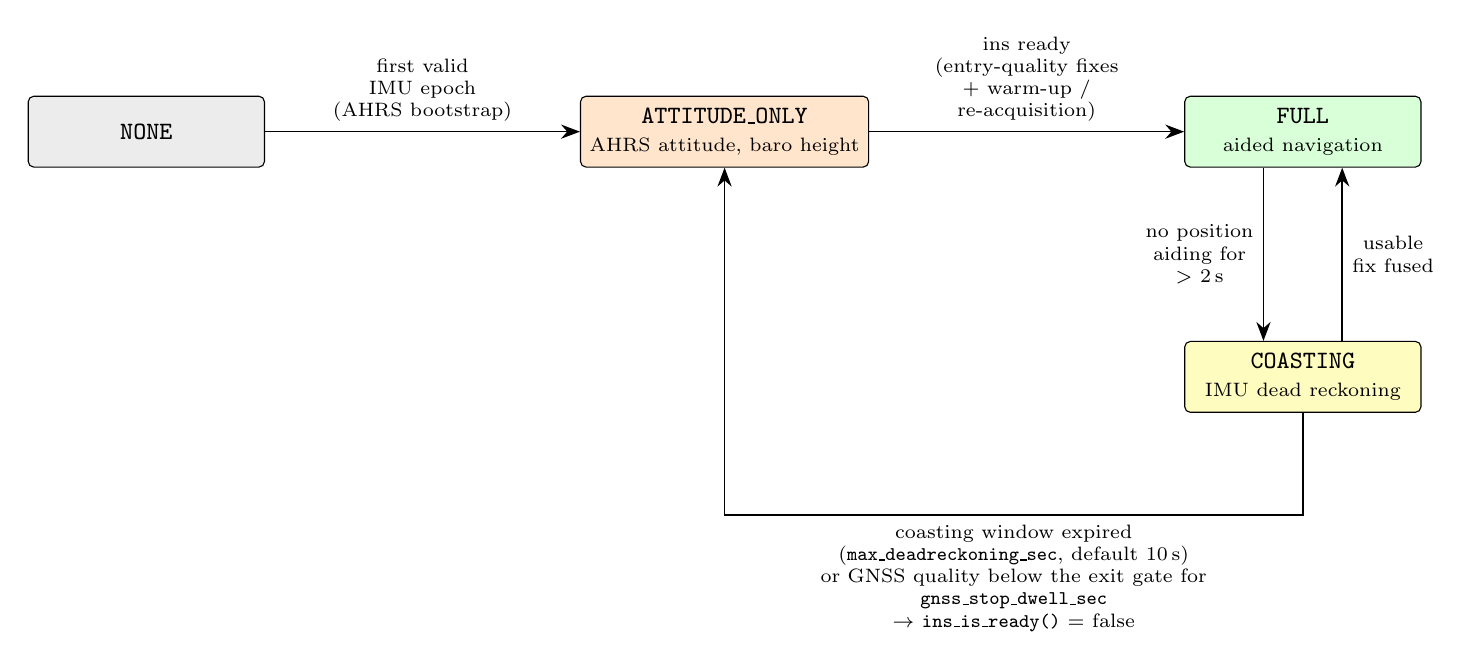
\begin{tikzpicture}[
  node distance=22mm and 40mm,
  state/.style={draw, rounded corners=2pt, minimum height=9mm,
                minimum width=30mm, align=center, font=\small},
  arr/.style={-{Stealth[length=2.4mm]}, semithick},
  lab/.style={font=\scriptsize, align=center}
]
  \node[state, fill=gray!15]   (none) {\code{NONE}};
  \node[state, fill=orange!20, right=of none] (att)
    {\code{ATTITUDE\_\allowbreak{}ONLY}\\[-1pt]{\scriptsize AHRS attitude, baro height}};
  \node[state, fill=green!15, right=of att] (full)
    {\code{FULL}\\[-1pt]{\scriptsize aided navigation}};
  \node[state, fill=yellow!25, below=of full] (coast)
    {\code{COASTING}\\[-1pt]{\scriptsize IMU dead reckoning}};

  \draw[arr] (none) -- node[lab, above] {first valid\\IMU epoch\\(AHRS bootstrap)} (att);
  \draw[arr] (att) -- node[lab, above] {ins ready\\(entry-quality fixes\\+ warm-up /\\re-acquisition)} (full);

  % FULL <-> COASTING: vertically stacked, one arrow each side of the gap
  \draw[arr] ([xshift=-5mm]full.south) --
    node[lab, left] {no position\\aiding for\\$>$ \SI{2}{\second}} ([xshift=-5mm]coast.north);
  \draw[arr] ([xshift=5mm]coast.north) --
    node[lab, right] {usable\\fix fused} ([xshift=5mm]full.south);

  % COASTING -> ATTITUDE_ONLY: routed through a clear lane below both boxes
  % so the long label never crosses a state box.
  \draw[arr] (coast.south) -- ++(0,-13mm) -| (att.south);
  \coordinate (mid)  at ($(att.south)!0.5!(coast.south)$);
  \coordinate (lane) at ([yshift=-13mm]coast.south);
  \node[lab, below] at (mid |- lane)
    {coasting window expired\\(\code{max\_\allowbreak{}deadreckoning\_\allowbreak{}sec}, default \SI{10}{\second})\\or GNSS quality below the exit gate for\\\code{gnss\_\allowbreak{}stop\_\allowbreak{}dwell\_\allowbreak{}sec}\\$\rightarrow$ \code{ins\_\allowbreak{}is\_\allowbreak{}ready()} = false};
\end{tikzpicture}
\caption{Solution-mode state machine (\code{nav\_\allowbreak{}suite\_\allowbreak{}get\_\allowbreak{}mode}). The way
out of \code{ATTITUDE\_\allowbreak{}ONLY} depends on which cause put it there, and both
require the fix stream to satisfy the entry-quality gate and its dwell
(\code{gnss\_\allowbreak{}start\_\allowbreak{}max\_\allowbreak*}, \code{gnss\_\allowbreak{}init\_\allowbreak{}dwell\_\allowbreak{}sec}). After an expired
coasting window the first usable fix \emph{re-acquires}: it re-anchors position
and velocity while attitude and IMU biases are kept, and the suite returns
directly to \code{FULL} with no warm-up. After a quality loss the instance was
torn down, so the return is a full re-bootstrap -- new position and velocity,
attitude re-seeded from the ARS/AHRS (heading from the magnetometer-AHRS, or
from the pre-outage heading advanced by the ARS, \S\ref{sec:suite}), IMU biases
carried over with inflated uncertainty -- and readiness waits out the usual
warm-up. The n-frame origin is carried over too, so local NED coordinates mean
the same thing before and after the outage. Only a fix the platform could not
have reached while unobserved -- further from the last known position than a
hard speed bound allows over the elapsed time -- falls back to anchoring a fresh
origin. Distance to the origin does not enter that decision: it is just how far
the mission has travelled. \code{allow\_\allowbreak{}unlimited\_\allowbreak{}deadreckoning} disables the
coasting-window cause; \code{gnss\_\allowbreak{}stop\_\allowbreak{}disable} disables the quality-loss
cause, and \code{auto\_\allowbreak{}reacquire\_\allowbreak{}disable} disables the tear-down, falling back
to holding \code{ins\_\allowbreak{}is\_\allowbreak{}ready()} down while the filter runs on.}
\label{fig:modes}
\end{figure}

\begin{figure}[htbp]
\centering
\resizebox{0.97\textwidth}{!}{%
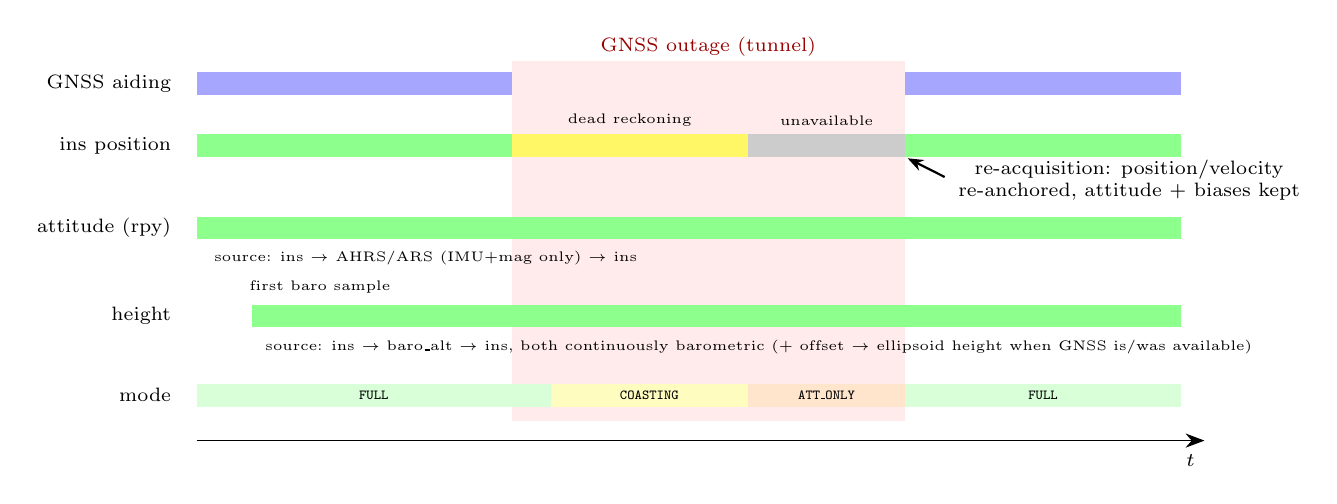
\begin{tikzpicture}[
  xscale=1.0, yscale=0.72,
  lab/.style={font=\scriptsize, anchor=east},
  note/.style={font=\scriptsize, align=center}
]
  % outage band (background)
  \begin{scope}[on background layer]
    \fill[red!8] (4,1.25) rectangle (9,7.6);
  \end{scope}
  \node[note, red!60!black] at (6.5,7.85) {GNSS outage (tunnel)};

  % --- row: GNSS aiding
  \node[lab] at (-0.2,7.2) {GNSS aiding};
  \fill[blue!35]  (0,7.0) rectangle (4,7.4);
  \fill[blue!35]  (9,7.0) rectangle (12.5,7.4);

  % --- row: ins position
  \node[lab] at (-0.2,6.1) {ins position};
  \fill[green!45]  (0,5.9) rectangle (4,6.3);
  \fill[yellow!60] (4,5.9) rectangle (7,6.3);
  \fill[gray!40]   (7,5.9) rectangle (9,6.3);
  \fill[green!45]  (9,5.9) rectangle (12.5,6.3);
  \node[note] at (5.5,6.55) {\tiny dead reckoning};
  \node[note] at (8,6.55)   {\tiny unavailable};
  % re-acquisition annotation (in the free band below the position row)
  \draw[-{Stealth[length=2mm]}, thick] (9.5,5.55) -- (9.03,5.88);
  \node[note, anchor=west] at (9.55,5.5)
    {re-acquisition: position/velocity\\re-anchored, attitude + biases kept};

  % --- row: attitude
  \node[lab] at (-0.2,4.65) {attitude (rpy)};
  \fill[green!45] (0,4.45) rectangle (12.5,4.85);
  \node[note, anchor=west] at (0.1,4.12)
    {\tiny source: ins $\rightarrow$ AHRS/ARS (IMU+mag only) $\rightarrow$ ins};

  % --- row: height
  \node[lab] at (-0.2,3.1) {height};
  \fill[green!45] (0.7,2.9) rectangle (12.5,3.3);
  \node[note, anchor=south west] at (0.55,3.32)
    {\tiny first baro sample};
  \node[note, anchor=west] at (0.75,2.55)
    {\tiny source: ins $\rightarrow$ baro\_alt $\rightarrow$ ins, both continuously barometric (+ offset $\rightarrow$ ellipsoid height when GNSS is/was available)};

  % --- row: mode
  \node[lab] at (-0.2,1.7) {mode};
  \fill[green!15]  (0,1.5)   rectangle (4.5,1.9);
  \fill[yellow!25] (4.5,1.5) rectangle (7,1.9);
  \fill[orange!20] (7,1.5)   rectangle (9,1.9);
  \fill[green!15]  (9,1.5)   rectangle (12.5,1.9);
  \node[font=\tiny] at (2.25,1.7)  {\code{FULL}};
  \node[font=\tiny] at (5.75,1.7)  {\code{COASTING}};
  \node[font=\tiny] at (8,1.7)     {\code{ATT\_\allowbreak{}ONLY}};
  \node[font=\tiny] at (10.75,1.7) {\code{FULL}};

  % time axis
  \draw[-{Stealth[length=2.4mm]}] (0,0.9) -- (12.8,0.9)
    node[below left=0.5mm and 0mm, font=\scriptsize] {$t$};
\end{tikzpicture}%
}
\caption{Graceful degradation across a GNSS outage. The AHRS/ARS filters
(IMU+mag only) and the baro\_alt filter (baro+accel+attitude) keep running
unconditionally, so attitude and -- with barometer data -- height stay available
throughout. Both switch sources across the outage (attitude: ins $\rightarrow$
AHRS/ARS $\rightarrow$ ins, height: ins $\rightarrow$ baro\_alt $\rightarrow$
ins, since the accessors prefer ins only in \code{FULL} mode). The barometric
height source does not remove that switch, it makes it benign: both sides are
then the same barometric quantity on the same vertical datum rather than a
GNSS-derived height handing over to a barometric one, so the remaining step is
the disagreement between two independent estimators of one quantity -- which the
suite cross-checks continuously. ins's horizontal position coasts on the IMU,
degrades after the coasting window, and re-acquires with the first fix.}
\label{fig:degradation}
\end{figure}

All local heights share one vertical datum (the ins NED origin).
Whichever filter initialises first defines it: if ins is ready when
the first pressure sample arrives, baro\_alt anchors at the current NED
height. If baro\_alt was running first (auto-init with a late first
fix), the ins origin is shifted vertically at bootstrap
(\S\ref{sec:origin-shift}) so the local heights agree, while the
absolute solution is untouched. This alignment is what keeps ins's own
barometric height (once selected as the height source) and baro\_alt's
independently-computed height consistent from the first shared epoch
onward, the two still carry separate accelerometer-bias states and are
not expected to stay bit-identical over a long run, only to track the
same physical quantity closely. Since the height accessors hand over
between exactly these two estimates at a mode change, the suite does not
assume they stay close -- it compares them every epoch and warns on a
persistent gap, alongside the same cross-check on the vertical velocity
(the two catch different failures: a divergence too slow to trip the
velocity bound still integrates into an unbounded height gap).

\subsection{Robustness policy}
\label{sec:robust}

Three layers protect the state estimate, uniformly across all filters,
following common navigation filter best practices \cite{carpenter2018}:

\begin{enumerate}
  \item \textbf{NaN/Inf boundary screening.} Every comparison with NaN
        is false, so NaN passes through gates written as
        \code{if (x <= limit) reject;}. One corrupt sample would poison
        the state and force the health check to shut the filter down.
        Therefore all inputs are checked with \code{isfinite()} at the
        API boundary; corrupt blocks are invalidated and counted
        (\code{n\_\allowbreak{}invalid\_\allowbreak{}input}), processing continues. Finiteness is
        not the only way an input can be wrong: absolute headings (the
        yaw measurement and the attitude hint) are accepted in any
        single-turn convention -- $[-\pi,\pi]$, $[0,2\pi)$ -- and
        normalised to $[-\pi,\pi]$, whereas a heading beyond one full
        turn is a unit or unwrapping error (degrees written into a
        radian field, an accumulated course) and is rejected and counted
        rather than wrapped into a plausible-looking but wrong heading.
  \item \textbf{Statistical screening with two policies.} Each scalar
        measurement row is tested with a Mahalanobis (chi-square) gate
        inside the UDU update (\S\ref{sec:robust-udu}). \emph{Persistent
        absolute references} (GNSS, magnetometer, absolute yaw,
        barometer) are \emph{downweighted} -- their noise is inflated so
        the gate is met -- never skipped: a skip policy would deadlock
        when a persistent offset exceeds an optimistic prior (the
        measurement is rejected forever while the covariance never
        shrinks). \emph{High-rate local references} (lighthouse, UWB,
        mocap) are \emph{skipped} on outliers: they glitch (occlusion,
        reflections) and a dropped sample is cheap at their rate.
  \item \textbf{Health check.} After each epoch the state and the
        covariance factors are checked for finiteness and non-negative
        variances. A tripped check marks the filter uninitialised
        instead of publishing corrupt values; in the suite the AHRS and
        baro filters then re-bootstrap autonomously from the stream.
\end{enumerate}

A fourth case is neither a corrupt value nor an outlier but a broken
\emph{timebase}: the sensor source reboots and its timestamp counter starts
over, so every following epoch is stamped far in the past. Each is correctly
dropped as older than \code{INS\_\allowbreak{}MAX\_\allowbreak{}DELAY\_\allowbreak{}MS}, but the drop happens before
the prediction step, so the internal time reference stays in the abandoned
timebase, the next epoch measures the same negative delta, and the filter stays
inert forever while still being fed good data. The filter therefore counts
\emph{consecutive} drops of this kind and, once the run reaches
\code{INS\_\allowbreak{}TIME\_\allowbreak{}RESTART\_\allowbreak{}EPOCHS}, forces the same defined reset as an
oversized forward jump and re-arms into the collecting state
(\code{n\_\allowbreak{}time\_\allowbreak{}restart\_\allowbreak{}reset}). Any epoch inside the tolerated depth clears
the run, which separates a restart from ordinary reordering: reordering arrives
in bursts, a restart never ends. Unlike a forward jump, this reset is not
suppressed by \code{allow\_\allowbreak{}unlimited\_\allowbreak{}deadreckoning} -- coasting would wait for
a timebase that never returns.

Drivers should not let it get that far. A driver reconstructing a 64-bit
timeline from a narrower counter (as \code{tools/insrcv.c} does from a 32-bit
microsecond source) can tell an overflow from a restart by \emph{where} in its
range the counter was, and stitch a restart onto the timeline it has already
emitted; the filter then keeps its converged state. Discriminating on step size
alone cannot: a restart from a high counter value is indistinguishable from an
overflow, and one from a low value looks like no anomaly at all.

\subsection{Memory and timing design}

Everything is statically sized. The dominating consumer in
\code{ins\_\allowbreak{}t} is the history ring buffer (30 entries $\times$
UDU factors); with the default compile-time maximum of 18 states the
struct is $\approx$\SI{50}{\kibi\byte}, with
\code{INS\_\allowbreak{}UNKNOWNS\_\allowbreak{}MAX=15} $\approx$\SI{38}{\kibi\byte}.
Per-epoch loops are bounded by compile-time constants or the runtime
state count $n \le$ \code{INS\_\allowbreak{}UNKNOWNS\_\allowbreak{}MAX}. Slowly varying Earth
quantities (curvature radii, $\Rne$, gravity) are cached and refreshed
only every \SI{100}{\metre} of travel. The per-step
latitude/longitude/height bookkeeping then costs some double
multiply-adds (\S\ref{sec:llh}).

\subsection{Sensor noise defaults}
\label{sec:defaults}

Any noise/tuning field left at zero is replaced by a
conservative consumer-MEMS default (MPU6050/BMI160 class), so an
uncharacterised sensor yields a stable (slightly cautious)
filter instead of an overconfident one, but is not optimally tuned. The \emph{gyro} defaults (ARW
density, bias random walk) are shared between ins and ahrs via
\code{sensor\_\allowbreak{}defaults.h}: in the suite both filters observe the same
physical gyro, so their fallback must agree. The \emph{accelerometer}
defaults are deliberately \emph{not} shared -- each filter fuses a
different physical quantity:
ins integrates the raw specific force (pure VRW density,
$\approx\!350\,\mu g/\sqrt{\text{Hz}}$), ars/ahrs fuses a discrete leveling
correction whose noise doubles as a manoeuvre-rejection margin
(\SI{0.25}{\metre\per\second\squared}), baro\_alt propagates an
attitude-projected vertical acceleration whose noise also absorbs
roll/pitch projection error
(\SI{0.025}{\metre\per\second\squared\per\sqrt{\hertz}},
$\approx$7$\times$ ins's density -- empirically not
interchangeable).
% ==============================================================================
\section{Estimation backend: UDU factorisation}
% ==============================================================================
\label{sec:udu}

All filters\footnote{Except the 1-state local-height/GNSS offset filter, where
the covariance is a plain scalar variance and the Kalman equations are
written out directly.} keep the covariance factorised as
\begin{equation}
  \mat{P} = \mat{U}\,\diag(\vect{d})\,\mat{U}\T ,
\end{equation}
with $\mat{U}$ unit upper triangular. In single precision a full
$\mat{P}$ update loses symmetry and positive definiteness quickly; the
factorised form is roughly equivalent to doubling the working precision
and guarantees $\mat{P} \succeq 0$ by construction
\cite{bierman1977,grewal2015,carpenter2018}.

\paragraph{Prediction (Thornton).}
The time update
\begin{equation}
  \mat{P}^- = \mat{\Phi}\,\mat{P}^+\,\mat{\Phi}\T
            + \mat{G}\,\diag(\vect{Q})\,\mat{G}\T
  \label{eq:thornton}
\end{equation}
is performed directly on the factors with Thornton's modified weighted
Gram--Schmidt orthogonalisation (\code{kalman\_\allowbreak{}udu\_\allowbreak{}predict}). Process
noise enters in \emph{noise-input form}: $\mat{G}$ maps physical white
noise sources (sensor noise, bias random walks, per-state extra noise)
onto the error states and $\vect{Q}$ holds the corresponding
variances.

\paragraph{Measurement update (Bierman).}
Every fusion step assumes a linear(ised) measurement model
\begin{equation}
  \vect{z} = \mat{H}\,\vect{x} + \vect{v},
  \qquad \vect{v} \sim \mathcal{N}(\vect{0}, \mat{R}),
  \label{eq:measmodel}
\end{equation}
relating the state $\vect{x}$ to the measurement $\vect{z}$ through the
observation matrix $\mat{H}$ and zero-mean noise $\vect{v}$ of covariance
$\mat{R}$; for the error-state filters (ins, ahrs) $\vect{x}$ in
\eqref{eq:measmodel} is the error state $\delta\vect{x}$, see
\eqref{eq:signconv} below. Measurements are processed as sequential
scalar rows (Bierman rank-one updates, \code{kalman\_\allowbreak{}udu}). For one
scalar row with measurement vector $\vect{h}$ (a row of $\mat{H}$),
residual $z$ and measurement variance $R$, the classical Kalman fusion
equations are
\begin{equation}
  \vect{k} = \frac{\mat{P}\,\vect{h}}{\vect{h}\T\mat{P}\vect{h} + R},
  \qquad
  \delta\vect{x} \leftarrow \delta\vect{x} + \vect{k}\,z,
  \qquad
  \mat{P} \leftarrow (\mat{I} - \vect{k}\,\vect{h}\T)\,\mat{P},
  \label{eq:kalmanfusion}
\end{equation}
with $\vect{k}$ the Kalman gain. \code{kalman\_\allowbreak{}udu} never forms
\eqref{eq:kalmanfusion} explicitly: it produces the same $\vect{k}$ and
$\delta\vect{x}$ update while propagating the covariance change directly
through the $\mat{U}$, $\vect{d}$ factors (Bierman's rank-one algorithm),
which avoids the numerically fragile
$\mat{P} \leftarrow (\mat{I}-\vect{k}\vect{h}\T)\mat{P}$ subtraction.
Rows with correlated noise are decorrelated
first: if the supplied $m\times m$ measurement covariance $\mat{R}$ has
off-diagonal entries, $\vect{z}$, $\mat{H}$ and $\mat{R}$ are whitened
with the Cholesky factor of $\mat{R}$ (\code{decorrelate()}), after
which the scalar updates see independent unit-variance measurements.

\paragraph{Robust update.}
\label{sec:robust-udu}
Each scalar row is screened with a chi-square test on its normalised
innovation before it is applied \cite{chang2014}: with innovation $z$,
innovation variance $S = \mat{h}\T\mat{P}\mat{h} + R$ and threshold
$\chi^2_{\text{th}}$,
\begin{equation}
  \frac{z^2}{S} > \chi^2_{\text{th}}
  \quad\Longrightarrow\quad
  \text{either skip the row, or inflate } R \text{ such that }
  \frac{z^2}{\mat{h}\T\mat{P}\mat{h} + R'} = \chi^2_{\text{th}} .
\end{equation}
The choice between \emph{skip} and \emph{downweight} (inflate) is the
per-measurement-type policy of \S\ref{sec:robust}. A downweighted gross
outlier receives a near-zero gain, but the measurement keeps
contributing information, so a persistent offset is eventually followed
instead of deadlocking the filter.

\paragraph{Error-state pattern.}
ins and ahrs are \emph{error-state} (indirect) filters: the nominal
state (quaternion, position, \dots) is propagated by nonlinear
mechanisation equations, while the Kalman filter estimates the small
error $\delta\vect{x}$ with linear(ised) dynamics. The error state is
implicitly zero after every update, so the Thornton step propagates only
the covariance, and each fusion computes a correction
$\delta\vect{x}$ that is immediately absorbed into the nominal state.
The sign convention throughout the library is
\begin{equation}
  \delta\vect{x} = \vect{x}_{\text{nominal}} - \vect{x}_{\text{true}},
  \qquad
  \vect{x}_{\text{nominal}} \leftarrow \vect{x}_{\text{nominal}}
  - \delta\vect{x} .
  \label{eq:signconv}
\end{equation}
Residuals are formed as $z = h(\vect{x}_{\text{nominal}}) -
z_{\text{measured}}$, which makes $z = \mat{H}\,\delta\vect{x} + v$
directly.

% ==============================================================================
\section{ins: the navigation ESKF}
% ==============================================================================

\subsection{State definition}

\paragraph{Nominal (total) state.} Float-only, in the local n-frame:
\begin{center}
\begin{tabular}{@{}llll@{}}
\toprule
Symbol & Field & Frame & Unit \\
\midrule
$\vect{p}$ & \code{pos\_\allowbreak{}local} & NED, relative to origin & \si{\metre} \\
$\vect{v}$ & \code{vel\_\allowbreak{}ned}   & NED & \si{\metre\per\second} \\
$\qbn$     & \code{qbn}        & body$\to$NED & -- \\
$\vect{b}_a$ & \code{acc\_\allowbreak{}bias} & body & \si{\metre\per\second\squared} \\
$\vect{b}_g$ & \code{gyr\_\allowbreak{}bias} & body & \si{\radian\per\second} \\
$\vect{b}_m$ & \code{mag\_\allowbreak{}bias} & body (for 18-state mode) & \si{\micro\tesla} \\
\bottomrule
\end{tabular}
\end{center}
The absolute position is anchored in double precision: the n-frame
origin in ECEF, and the current latitude/longitude/height
$(\varphi,\lambda,h)$ bookkept incrementally (\S\ref{sec:llh}).

\paragraph{Error state.} 15 elements, extended to 18 when magnetometer
hard-iron bias estimation is enabled per instance at init:
\begin{equation}
  \delta\vect{x} =
  \begin{bmatrix}
    \delta\vect{p}\T & \delta\vect{v}\T & \vect{\psi}\T &
    \delta\vect{b}_a\T & \delta\vect{b}_g\T &
    [\,\delta\vect{b}_m\T\,]
  \end{bmatrix}\T ,
\end{equation}
with $\vect{\psi}$ the small-angle attitude error in the n-frame
(\emph{psi-angle model}):
\begin{equation}
  \Rbn\big|_{\text{nominal}}
  = \left(\mat{I} + \cross{\vect{\psi}}\right)
    \Rbn\big|_{\text{true}} .
  \label{eq:psimodel}
\end{equation}
A correction is applied as a left (n-frame side) quaternion
multiplication $\vect{q} \leftarrow \vect{q}(-\vect{\psi}) \otimes
\vect{q}$ (\code{ins\_\allowbreak{}quat\_\allowbreak{}small\_\allowbreak{}angle\_\allowbreak{}correction}), consistent
with \eqref{eq:signconv}.

The 15/18 selection follows a \emph{runtime-$n$} pattern: all arrays are
dimensioned to the compile-time maximum \code{INS\_\allowbreak{}UNKNOWNS\_\allowbreak{}MAX}
(default 18), the active size $n$ is fixed per instance at init.
Memory-constrained integrations could override the maximum to 15 and
reclaim the storage, \code{ins\_\allowbreak{}init} then rejects the option instead
of corrupting memory.

\subsection{Strapdown mechanisation}
\label{sec:strapdown}

Each IMU epoch propagates the nominal state over $\dt$
(\code{ins\_\allowbreak{}strapdown}). Earth rotation and transport rate are
compensated:
\begin{align}
  \vect{\omega}^\nframe_{i\nframe}
    &= \vect{\omega}^\nframe_{i\eframe}
     + \vect{\omega}^\nframe_{\eframe\nframe}, &
  \vect{\omega}^\nframe_{i\eframe}
    &= \omega_E \begin{bmatrix} \cos\varphi \\ 0 \\ -\sin\varphi
       \end{bmatrix}, &
  \vect{\omega}^\nframe_{\eframe\nframe}
    &= \begin{bmatrix}
         v_E / (R_N + h) \\
         -v_N / (R_M + h) \\
         -v_E \tan\varphi / (R_N + h)
       \end{bmatrix},
\end{align}
with $\omega_E$ the WGS84 Earth rate and $R_M, R_N$ the meridian and
normal curvature radii. The body rate relative to the n-frame is
\begin{equation}
  \vect{\omega}^\bframe_{\nframe\bframe}
  = \underbrace{\tilde{\vect{\omega}}^\bframe_{i\bframe}
    - \vect{b}_g}_{\text{bias-corrected gyro}}
  - \left(\Rbn\right)\T \vect{\omega}^\nframe_{i\nframe} .
\end{equation}

\paragraph{Attitude.} The quaternion is advanced by the equivalent
rotation vector $\vect{\omega}^\bframe_{\nframe\bframe}\dt$,
implemented in \code{ins\_\allowbreak{}quat\_\allowbreak{}rotate} with a Taylor-series
expansion for numerical robustness near zero rotation
\cite{wendel2011}.

\paragraph{Velocity.} With the bias-corrected specific force
$\vect{f}^\bframe = \tilde{\vect{f}}^\bframe - \vect{b}_a$, the n-frame
correction terms
\begin{equation}
  \vect{a}_{\text{corr}}
  = \vect{g}^\nframe
  - \left(2\,\vect{\omega}^\nframe_{i\eframe}
        + \vect{\omega}^\nframe_{\eframe\nframe}\right)
    \times \vect{v}
\end{equation}
(gravity including centrifugal term, plus Coriolis), and a second-order
rotation (coning-style) correction of the integrated specific force
\cite{titterton2004,wendel2011}
\begin{equation}
  \Delta\vect{u}^\bframe
  = \vect{f}^\bframe\,\dt
  + \tfrac{1}{2}\,\vect{\omega}^\bframe_{\nframe\bframe}
    \times \vect{f}^\bframe\,\dt^2 ,
\end{equation}
the velocity update is
\begin{equation}
  \vect{v}_{k+1} = \vect{v}_k + \Rbn\big|_k\,\Delta\vect{u}^\bframe
                 + \vect{a}_{\text{corr}}\,\dt .
\end{equation}
Note that $\Rbn$ is evaluated at epoch $k$ (before the attitude update);
the rotation correction term accounts for the attitude motion across
the interval.

\paragraph{Position.} Trapezoidal integration:
\begin{equation}
  \vect{p}_{k+1} = \vect{p}_k
  + \tfrac{1}{2}\,\dt\left(\vect{v}_k + \vect{v}_{k+1}\right).
\end{equation}

\subsection{Incremental absolute-position bookkeeping}
\label{sec:llh}

The filter states are float in the local n-frame, the absolute
$(\varphi, \lambda, h)$ is maintained in double precision from the
\emph{applied} n-frame deltas:
\begin{equation}
  \Delta\varphi = \frac{\Delta p_N}{R_M + h}, \qquad
  \Delta\lambda = \frac{\Delta p_E}{(R_N + h)\cos\varphi}, \qquad
  \Delta h = -\Delta p_D .
\end{equation}
The curvature terms (and $\Rne$, gravity) change only by
$\sim d / R_{\text{earth}}$ per metre of travel and are cached,
refreshed after every \SI{100}{\metre} of accumulated travel. This keeps
the double-precision cost at two multiply-adds per step while avoiding
the classic float breakdown of absolute coordinates ($\sim$\SI{0.5}{\metre}
resolution at Earth radius in single precision).

\subsection{Covariance prediction}
\label{sec:predict}

The prediction is throttled: it runs when at least
\code{kalman\_\allowbreak{}update\_\allowbreak{}dt\_\allowbreak{}sec} has elapsed (default order
\SIrange{50}{100}{\milli\second}), not at IMU rate -- the error dynamics
are slow, and the strapdown already propagates the nominal state per
sample. The discrete transition matrix over the elapsed $\dt$ is
\cite[eq.~10.1]{wendel2011}
\begin{equation}
  \mat{\Phi} =
  \begin{bmatrix}
    \mat{I} & \mat{I}\dt & \mat{0} & \mat{0} & \mat{0} \\
    \mat{0} & \mat{I} & -\cross{\vect{f}^\nframe}\dt & -\Rbn\dt & \mat{0} \\
    \mat{0} & \mat{0} & \mat{I} & \mat{0} & -\Rbn\dt \\
    \mat{0} & \mat{0} & \mat{0} & \mat{I} & \mat{0} \\
    \mat{0} & \mat{0} & \mat{0} & \mat{0} & \mat{I}
  \end{bmatrix},
  \qquad
  \vect{f}^\nframe = \Rbn\,\vect{f}^\bframe ,
  \label{eq:phi}
\end{equation}
where $\vect{f}^\bframe$ is the latest bias-corrected specific force.
The $-\cross{\vect{f}^\nframe}$ block is the velocity/attitude coupling
under the sign convention \eqref{eq:signconv}\eqref{eq:psimodel}:
$\delta\dot{\vect{v}} = \cross{\vect{\psi}}\,\vect{f}^\nframe
= -\cross{\vect{f}^\nframe}\,\vect{\psi}$. In 18-state mode the
magnetometer bias block is appended as identity (random walk).

Process noise enters \eqref{eq:thornton} through
\begin{equation}
  \mat{G} =
  \left[
  \begin{array}{cccc|c}
    \mat{0} & \mat{0} & \mat{0} & \mat{0} & \multirow{5}{*}{$\mat{I}_{n}$} \\
    \Rbn & \mat{0} & \mat{0} & \mat{0} & \\
    \mat{0} & -\Rbn & \mat{0} & \mat{0} & \\
    \mat{0} & \mat{0} & \mat{I} & \mat{0} & \\
    \mat{0} & \mat{0} & \mat{0} & \mat{I} &
  \end{array}
  \right],
  \qquad
  \vect{Q} = \dt \cdot
  \begin{bmatrix}
    \text{PSD}_{\text{acc}} \\
    \text{PSD}_{\text{gyr}} \\
    \sigma^2_{b_a\text{-RW}} \\
    \sigma^2_{b_g\text{-RW}} \\
    \vect{q}_{xx}
  \end{bmatrix},
\end{equation}
i.e.\ twelve IMU noise inputs (accelerometer and gyro white noise
rotated into the n-frame, both bias random walks) plus $n$ per-state
extra-noise inputs $\vect{q}_{xx}$ (position/velocity/attitude
stabilisation noise and, in 18-state mode, the magnetometer-bias random
walk). The measurement-supplied per-axis PSDs are used when present,
axes left at zero fall back to the conservative MEMS defaults
(\S\ref{sec:defaults}) rather than injecting zero process noise.

\subsection{Measurement models}

All fusions follow the pattern of \S\ref{sec:udu}: build the residual
$\vect{z} = h(\text{nominal}) - \vect{z}_{\text{meas}}$ and the Jacobian
$\mat{H}$, run the robust Bierman update, subtract the estimated
$\delta\vect{x}$ from the nominal state.

\subsubsection{GNSS position}
\label{sec:gnss-pos}

The measurement arrives in ECEF (double) with a full $3\times 3$ NED
covariance. It is converted to $(\varphi,\lambda,h)$ once per epoch (the
only double-precision math in the fusion path), differenced against the
filter's anchor at the measurement's time of validity, and mapped to
metres with the curvature radii. With the GNSS antenna lever arm
$\vect{l}^\bframe$:
\begin{equation}
  \vect{z}_p = \underbrace{\mathcal{M}\!\left(
      (\varphi,\lambda,h)_{\text{tov}} -
      (\varphi,\lambda,h)_{\text{meas}}\right)}_{\text{NED difference}}
  + \Rbn\big|_{\text{tov}}\,\vect{l}^\bframe ,
\end{equation}
\begin{equation}
  \mat{H}_p =
  \begin{bmatrix}
    \mat{I}_3 & \mat{0} & -\cross{\vect{l}^\nframe} & \mat{0} & \mat{0}
  \end{bmatrix},
  \qquad \vect{l}^\nframe = \Rbn\big|_{\text{tov}}\,\vect{l}^\bframe ,
  \label{eq:Hpos}
\end{equation}
following \cite[eq.~8.62]{wendel2011}. The $-\cross{\vect{l}^\nframe}$
block makes a lever-arm-induced residual observable in the attitude
states: without it, the filter would attribute the residual purely to a
position error and could not extract heading/tilt information from an
offset antenna.

Quality gates reject measurements whose reported standard deviations
exceed configured horizontal/vertical limits before fusion (counted in
the diagnostics). When \code{ins} uses the barometric height source
(\S\ref{sec:baro-height-meas}), only the horizontal ($N,E$) rows of
\eqref{eq:Hpos} are fused -- the vertical row is dropped, not
downweighted: the two height sources are not simultaneous alternatives
for the same epoch, the selection is fixed once at bootstrap. The
position gates then grade the fix on its horizontal accuracy alone, both
here and at the 3D exit gate (\S\ref{sec:readiness}): a fix whose
vertical row is discarded before fusion must not lose the horizontal
solution its aiding, nor drop the whole 3D solution, over an accuracy it
no longer contributes - a good HDOP with a poor VDOP is a typical
satellite geometry. The velocity gates are unaffected on all three axes,
as is the \emph{entry} gate's vertical position limit: the entry gate
runs during a cold bootstrap, before any height source is latched, and
that one fix defines the origin, so its vertical accuracy is the
accuracy of the absolute vertical datum whatever runs on top of it
afterwards.

\subsubsection{Barometric height (ins-internal)}
\label{sec:baro-height-meas}

If barometer data was present when \code{ins} bootstrapped
(\S\ref{sec:auto-init}), the barometric altitude is fused directly as a
scalar measurement of the vertical position state, on the same datum
anchor $h_0$ established at bootstrap (\S\ref{sec:origin-shift},
\S\ref{sec:heightsystems}) and using the same ISA conversion as
\code{baro\_\allowbreak{}alt} \eqref{eq:isa}:
\begin{equation}
  z_h = -p_z - \big(h_{\text{ISA}}(p) - h_0\big),
  \qquad
  \mat{H}_h = \begin{bmatrix}
    -\vect{e}_3\T & \mat{0} & \mat{0} & \mat{0} & \mat{0}
  \end{bmatrix},
  \label{eq:Hbaroheight}
\end{equation}
with $\vect{e}_3 = (0,0,1)\T$ picking the down component of $\vect{p}$
(recall $h = -p_z$, \S\ref{sec:heightsystems}). Fused through the same
robust UDU update as every other measurement (\S\ref{sec:udu}), outliers
downweighted like the barometer's own fusion in \code{baro\_\allowbreak{}alt}
(\S\ref{sec:baroalt}) -- a persistent absolute reference, not a
high-rate local one (\S\ref{sec:robust}). This replaces, not
supplements, the vertical row of the GNSS position measurement
\eqref{eq:Hpos} for the lifetime of the filter instance: the choice of
height source is made once, at bootstrap, from whether a barometer was
observed (\S\ref{sec:auto-init}), not re-evaluated per epoch. GNSS
velocity (\S\ref{sec:gnss-vel}), including its vertical component, is
fused unconditionally either way (\S\ref{sec:decisions}).

Like every other fusion this runs on live epochs only: while the
coasting window is expired the filter is inert
(\S\ref{sec:readiness}). The barometer keeps being cached across such
an outage, and the height is picked back up from it at the
re-acquisition, which is what keeps the vertical solution continuous
across a passage the frozen state knew nothing about.

\subsubsection{GNSS velocity}
\label{sec:gnss-vel}

NED velocity with full covariance; the lever-arm velocity is
compensated and its attitude coupling included
\cite[eq.~8.74]{wendel2011}:
\begin{equation}
  \vect{z}_v = \vect{v}_{\text{tov}}
  + \Rbn\big|_{\text{tov}}
    \left(\vect{\omega}^\bframe_{\nframe\bframe} \times
    \vect{l}^\bframe\right)
  - \vect{v}_{\text{meas}} ,
  \qquad
  \mat{H}_v =
  \begin{bmatrix}
    \mat{0} & \mat{I}_3 &
    -\cross{\Rbn(\vect{\omega}^\bframe\times\vect{l}^\bframe)} &
    \mat{0} & \mat{0}
  \end{bmatrix}.
\end{equation}
(Using  $\vect{\omega}^\bframe_{i\bframe}$ instead of
$\vect{\omega}^\bframe_{\nframe\bframe}$ neglects the Earth/transport rate
crossed with the GNSS antenna lever arm, $\sim$\SI{0.1}{\milli\metre\per\second} for
a \SI{1}{\metre} arm -- negligible against GNSS velocity noise.) When
position and velocity are fused together, an optional
position/velocity cross-covariance block completes the full $6\times 6$
measurement covariance, correlated blocks are whitened before the
scalar updates (\S\ref{sec:udu}).

\subsubsection{GNSS covariance conditioning}
\label{sec:gnss-cond}

A receiver's reported covariance is not fused as it stands. It passes a fixed
pipeline whose knobs live under \code{gnss:} in \code{config.yaml}
(\S\ref{sec:configyaml}), applied per epoch to the position and velocity blocks
before either reaches \eqref{eq:Hpos}:
\begin{equation}
  \text{envelope} \rightarrow \text{scale} \rightarrow
  \text{height scale} \rightarrow \text{floor} \rightarrow \text{cap}
  \rightarrow \text{manoeuvre term} .
\end{equation}
\begin{description}\setlength\itemsep{0pt}
  \item[Envelope.] A rise in the reported $1\sigma$ takes effect at once, a
    fall only with a first-order decay of \code{acc\_\allowbreak{}envelope\_\allowbreak{}tau\_\allowbreak{}sec}:
    $e \leftarrow \max(\sigma_{\text{rep}},\, e\,(1-\alpha))$,
    $\alpha = \operatorname{clamp}(\dt/\tau, 0, 1)$, kept per block and axis
    group. A receiver's accuracy figure returns to nominal well before a
    re-acquired fix has settled.
  \item[Scale and height scale.] $\mat{Q} \leftarrow s^2\mat{Q}$, plus an extra
    downweight of the position Down axis applied as the correlation-preserving
    congruence $\diag(1,1,s_h)\,\mat{Q}\,\diag(1,1,s_h)$.
  \item[Floor and cap.] Per-axis clamps of the diagonal (horizontal/vertical
    separately), so a floored or capped axis picks up (or loses) independent
    variance on that axis alone. The cap is what makes the loose fusion gate
    safe: \code{gnss\_\allowbreak{}max\_\allowbreak*} defaults to the caps, so a degraded fix is
    downweighted rather than discarded while the unbounded reported accuracy
    stays out of the 32-bit hot path.
  \item[Manoeuvre term.] Extra independent variance on the velocity diagonal,
    $\sigma_{\text{extra}} = k \lVert \vect{a} \rVert$, from the windowed
    n-frame acceleration of the \emph{antenna} -- the body's plus the
    centripetal term $\vect{\omega}\times(\vect{\omega}\times\vect{l})$ of the
    lever arm. A Doppler velocity averages over the receiver's measurement
    interval $T$ while the state is instantaneous, so under acceleration the
    two differ by about $aT/2$, an error the reported accuracy cannot describe
    because it belongs to the platform rather than to the signal.
\end{description}
All of it weights the \emph{fusion} only. Every fix-quality gate
(\S\ref{sec:readiness}) keeps grading the stddev the receiver reported, so
downweighting a noisy receiver can never turn into refusing to use it.

\subsubsection{Absolute speed (odometry, OBD-II)}
\label{sec:speed}

A scalar ground speed -- an OBD-II vehicle speed, a wheel-odometry pulse
rate, a Doppler log -- is the magnitude of the velocity with no direction
attached:
\begin{equation}
  h(\vect{x}) = \left\lVert \vect{v}^\nframe \right\rVert , \qquad
  z_s = \left\lVert \vect{v}_{\text{tov}} \right\rVert - z_{\text{meas}} , \qquad
  \mat{H}_s =
  \begin{bmatrix}
    \mat{0} & \hat{\vect{v}}\T & \mat{0} & \mat{0} & \mat{0}
  \end{bmatrix},
  \quad
  \hat{\vect{v}} = \frac{\vect{v}^\nframe}{\left\lVert \vect{v}^\nframe \right\rVert} .
\end{equation}
The nonlinearity costs nothing in an error-state filter: the residual is
formed from the nonlinear $h(\cdot)$ evaluated on the \emph{nominal}
state and $\mat{H}$ is only its Jacobian with respect to the error state,
exactly as for every other reference here.

$\hat{\vect{v}}\T$ picks out the component of the velocity error \emph{along the
current direction of travel} and nothing else; cross-track error is invisible to
a quantity that carries no direction. The along-track component is nevertheless
the one that runs away first when GNSS stops, since attitude and
accelerometer-bias errors leak into velocity through the strapdown and it is the
integrated velocity error that becomes position error. One scalar per second
therefore buys most of what a GNSS-denied stretch needs, without the state
cloning a delta-position (wheel-tick) formulation would require.

Two properties of the sensor class shape the implementation. First,
$\hat{\vect{v}}$ is undefined at $\vect{v}^\nframe = \vect{0}$ and numerically
meaningless just above it, so the fusion is gated on a minimum \emph{filtered}
speed: what has to be well conditioned is the Jacobian, and that is built from
the state, not from the reading. A genuinely stopped platform is the automatic
ZUPT's job (\S\ref{sec:autozupt}).

Second, the error budget has two parts that scale differently, and
lumping them together would bias the filter. An OBD-II \code{PID 0x0D}
value is quantised to \SI{1}{\kilo\metre\per\hour}, a
\SI{0.080}{\metre\per\second} $1\sigma$ that does not grow with speed.
The vehicle's speedometer calibration does: EU type approval forbids
reading low, so a production speedometer reads \SIrange{2}{5}{\percent}
high, and tyre wear moves it further -- \SI{0.83}{\metre\per\second} at
\SI{100}{\kilo\metre\per\hour}, ten times the quantisation noise and
\emph{systematic}. A constant scale factor removes the calibrated part
and a relative variance prices what is left:
\begin{equation}
  z_{\text{meas}} = s_{\text{scale}}\, z_{\text{raw}} , \qquad
  R = \sigma_{\text{sample}}^2 + \left(k_{\text{rel}}\,
      z_{\text{meas}}\right)^2 .
\end{equation}
No scale-factor state is estimated: this stays a measurement-boundary
feature and leaves the runtime-selected state size untouched.

The reading is unsigned by contract (an OBD-II speed PID cannot express
reverse), so a negative value is treated as a unit or sign error and dropped
rather than taken as its magnitude. Latency is the norm on this input -- a
Bluetooth OBD-II round trip is tens of milliseconds -- and is handled by the
same history anchoring GNSS uses (\S\ref{sec:delayed}).

\subsubsection{Position decimation against an unknown correlation}
\label{sec:gnss-pos-decimation}

That optional cross-covariance block is the exception, not the rule. A
receiver computes position and velocity in one internally coupled
solution, but no common output message carries the correlation between
them: \code{gnss\_\allowbreak{}Qll\_\allowbreak{}pos\_\allowbreak{}vel\_\allowbreak{}ned} is filled only by the few receivers
that report it and is zero otherwise. Fusing both blocks every epoch as
if they were independent therefore counts one solution twice. The
covariance drops below what the measurements support, which in turn
shrinks the Kalman gain of every other aiding source and pushes the
difference into the accelerometer-bias and attitude states that are free
to absorb it.

\code{gnss.pos\_\allowbreak{}decimation} answers this by spending only one block per
epoch. With the factor $N$, every $N$-th epoch that offers a usable
position \emph{and} a usable velocity fuses the position alone, the other
$N-1$ fuse the velocity alone; $N \le 1$ restores the combined fuse. An
epoch offering only one of the two is never touched -- the decimation
removes information, it never adds any.

Decimation is deliberately the blunt instrument: it assumes nothing about a
correlation that cannot be observed, unlike an assumed correlation coefficient,
which is unverifiable against a receiver that reports none and drives $\mat{R}$
towards singularity when guessed too high. It also attacks the second, larger
correlation in the same data: a receiver's position error is dominated by
multipath, residual ionospheric delay and its own smoothing, all correlated over
minutes, while the Doppler-derived velocity is comparatively white. The textbook
cure for that time-correlated part is a Gauss-Markov position-bias state per
axis, which would allow full rate for both -- but that is a change to the state
vector, not what this option does.

Two cases suspend the decimation. While the coasting window is expired
(\S\ref{sec:readiness}) the position is the entire point of the fix,
so it is always fused and re-anchors the filter. And a position-aiding
gap longer than the fix-stream continuity bound restarts the cycle at a
position, because after a gap the dead-reckoned position is the stale
quantity. An epoch whose position is withheld still counts as position
aiding for the coasting window: the fix carried a usable position and the
filter declined to spend it, which is not the same as not having one.

\subsubsection{Local NED position}

Indoor references (e.\,g. Lighthouse/SteamVR, UWB, motion capture, total
station) measure \code{pos\_\allowbreak{}local} directly in the filter's n-frame --
same residual and Jacobian structure as \eqref{eq:Hpos}, without any
coordinate conversion. Frame alignment (origin offset + rotation into
NED) is the caller's responsibility. Outliers are \emph{skipped}, not
downweighted (\S\ref{sec:robust}).

\subsubsection{Absolute yaw}

A heading reference (dual-antenna GNSS, mocap pose, gyro compass) is
fused as a scalar residual on the yaw component of the attitude error:
\begin{equation}
  z_\psi = \operatorname{wrap}_{\pm\pi}
    \left(\hat{\psi}_{\text{tov}} - \psi_{\text{meas}}\right),
  \qquad
  \mat{H}_\psi = \begin{bmatrix}
    \mat{0} & \mat{0} & \vect{e}_3\T & \mat{0} & \mat{0}
  \end{bmatrix},
\end{equation}
since to first order a heading residual equals the yaw component of the
n-frame attitude error. Fusion is skipped near gimbal lock
($|\sin\theta| > 0.99$), where yaw is ill-defined.

\paragraph{Automotive mode (course-over-ground yaw).} Opt-in
(\code{automotive\_\allowbreak{}mode}), this reuses the same scalar update with
$\psi_{\text{meas}} = \operatorname{atan2}(v_E, v_N)$ from the GNSS
velocity vector, above a minimum ground speed
(\code{automotive\_\allowbreak{}min\_\allowbreak{}speed\_\allowbreak{}mps}, default \SI{2}{\metre\per\second} --
below it course over ground is not well defined). It assumes a
non-holonomic vehicle that travels in the direction it points --
reasonable for a car, wrong for a glider or a boat drifting sideways: in
coordinated flight the airframe's heading aligns with the
\emph{airspeed} vector, not the \emph{ground-track} vector GNSS
measures, so a crosswind adds a wind-drift (crab) angle independent of
speed -- raising the minimum speed does not fix this. The measurement
standard deviation is the velocity-noise-over-speed heading uncertainty,
floored (\code{automotive\_\allowbreak{}min\_\allowbreak{}yaw\_\allowbreak{}stddev}, default \SI{5}{\degree}) so
it never claims more precision than that assumption warrants. Raising
this floor (e.g.\ to a conservative crab-angle estimate such as
\SI{15}{\degree}) lets the fusion still act as a weak long-term anchor
against free-yaw drift on a platform where the assumption itself is
looser than a car's, without asserting automotive-grade heading
precision. Outliers (e.g.\ reversing, $\sim$\SI{180}{\degree} residual)
are chi-square-downweighted like any absolute yaw reference, never
dropped. An alternative to magnetometer heading aiding when none is
available.

\subsubsection{Magnetometer (yaw-only vector fusion)}
\label{sec:ins-mag}

The magnetometer is fused as a 3D vector measurement of the body-frame
field with model $\vect{m}^\bframe = (\Rbn)\T \vect{m}^\nframe +
\vect{b}_m$:
\begin{equation}
  \vect{z}_m = (\Rbn)\T\,\vect{m}^\nframe + \vect{b}_m
             - \tilde{\vect{m}}^\bframe .
\end{equation}
The full attitude Jacobian of this model would be
$(\Rbn)\T \cross{\vect{m}^\nframe}$ on the $\vect{\psi}$ block.
\emph{Deliberately, only the yaw column is kept:}
\begin{equation}
  \mat{H}_m[:,\psi_z] = (\Rbn)\T
    \left(\vect{m}^\nframe \times \vect{e}_D\right),
  \qquad
  \mat{H}_m[:,\psi_x] = \mat{H}_m[:,\psi_y] = \mat{0},
  \qquad
  \frac{\partial \vect{z}_m}{\partial \delta\vect{b}_m} = \mat{I}_3 .
\end{equation}
The zeroed roll/pitch columns ensure that magnetic dip and hard-iron /
deviation disturbances can never tilt the attitude estimate -- leveling
information comes exclusively from the accelerometer. The vector
measurement can only rotate the estimate about the vertical, residual
components that a yaw rotation cannot explain (magnitude or dip
mismatch) meet zero entries and produce no state update
\cite[eq.~10.7]{wendel2011}.

\paragraph{Hard-iron bias observability (18-state mode).} The bias term
is constant in the \emph{body} frame while the field term
$(\Rbn)\T\vect{m}^\nframe$ rotates with attitude. This makes
$\vect{b}_m$ separable from the yaw error -- but only under attitude
changes. Expect convergence during/after rotations, this is
why the bias is estimated \emph{inside} the filter, where the yaw/bias
cross-covariance is maintained, instead of in an external calibration
estimator.

\paragraph{Field-strength disturbance gate.} Once a position is known
(\S\ref{sec:wmm}), the measured magnitude is compared against the WMM
total field $B_{\text{WMM}}$. With relative deviation
$\epsilon = \big|\,\|\tilde{\vect{m}}\| - B_{\text{WMM}}\big| /
B_{\text{WMM}}$ and tolerance $\tau$ (default 0.30), a sample outside
the band has its per-axis noise inflated by $(\epsilon/\tau)^2$ --
downweighted, not dropped, per the persistent-reference policy. The
gate is defense-in-depth over the vector chi-square test (it bites when
the measurement noise is set loose) and can be disabled for
uncalibrated magnetometers. Fusion requires per-axis variances
(no default) and is rate-limited: it is skipped when the horizontal
reference field is unusable (magnetic poles).

\paragraph{Weight and rate limit: a long-term anchor, not a yaw sensor.}
Since only the yaw column survives, the length of that column is the
horizontal field $\|\vect{m}^\nframe_h\|$, so a per-axis noise
$\sigma_m$ acts as a heading measurement of roughly
\begin{equation}
  \sigma_\psi \approx \frac{\sigma_m}{\|\vect{m}^\nframe_h\|} .
\end{equation}
At mid-latitudes $\|\vect{m}^\nframe_h\| \approx
\SI{20}{\micro\tesla}$, so even a sensor-grade
$\sigma_m = \SI{3}{\micro\tesla}$ is already about
\SI{8.6}{\degree} of heading per sample -- and at a typical
\SI{10}{\hertz} output rate the filter accumulates that down to under a
degree within seconds. A MEMS gyro of
\SI{0.02}{\degree\per\second\per\sqrt{\hertz}} drifts far less than that
over the same seconds, so fusing at the sensor rate buys no heading
accuracy. What it does buy is exposure: motor currents and ferrous
structure bend the field by far more than $\sigma_m$, and those
disturbances are strongly time-correlated while the update treats every
sample as independent evidence, so a high rate systematically
over-counts a biased heading.

Both knobs therefore default weak, and both defaults live in the
library rather than in each harness: a sample that arrives with no
per-axis variance is fused with \code{INS\_\allowbreak{}DEFAULT\_\allowbreak{}MAG\_\allowbreak{}STDDEV\_\allowbreak{}UT}
(\code{sensor\_\allowbreak{}defaults.h}), a noise of the same order as the field
itself, i.e.\ $\sigma_\psi \approx \SI{1}{\radian}$ per sample, and the
rate limit defaults to \SI{1}{\hertz}
(\code{ins\_\allowbreak{}options\_\allowbreak{}t.magnetometer\_\allowbreak{}min\_\allowbreak{}delay\_\allowbreak{}ms}, 0 $\to$ default,
negative $\to$ off). That combination still binds the heading over
minutes, which is all the gyro needs, without letting a disturbed field
pull it within seconds. Note that this is a defence against
\emph{noise and transients only}: a standing hard-iron offset is a
\emph{bias}, and where the magnetometer is the only absolute heading
reference the steady-state error it causes is independent of $\sigma_m$
-- lowering the weight only stretches the time the filter takes to reach
the same wrong answer. (It does shift the balance once a second heading
source is present, e.g.\ GNSS course in automotive mode.) Bias is the
calibration's job
(\code{mag: fixed\_\allowbreak{}bias} / \code{estimate\_\allowbreak{}bias}), not the weighting's.

\subsubsection{Zero-velocity and zero-rotation updates (ZUPT/ZARU)}

On trigger (external flag or the automatic detector,
\S\ref{sec:autozupt}):
\begin{align}
  \text{ZUPT:} \quad
  \vect{z} &= \hat{\vect{v}}, &
  \mat{H} &= \begin{bmatrix}
    \mat{0} & \mat{I}_3 & \mat{0} & \mat{0} & \mat{0}
  \end{bmatrix}, \\
  \text{ZARU:} \quad
  \vect{z} &= \hat{\vect{b}}_g
    + (\Rbn)\T\vect{\omega}^\nframe_{i\nframe}
    - \bar{\vect{\omega}}_{\text{meas}}, &
  \mat{H} &= \begin{bmatrix}
    \mat{0} & \mat{0} & \mat{0} & \mat{0} & \mat{I}_3
  \end{bmatrix},
\end{align}
i.e.\ the zero-rotation update is a direct gyro-bias measurement, with
the Earth + transport rate seen in the body frame compensated. Both are
rate-limited to one fusion per Kalman period.
$\bar{\vect{\omega}}_{\text{meas}}$ is the gyro \emph{averaged over the
current stillness run} rather than a single sample: a momentary sample
of a vibrating-but-still platform (idling engine) would inject the
vibration directly into the gyro bias states -- with a tight
$\sigma_{\text{ZARU}}$ this corrupted the heading by up to
\SI{0.6}{\degree\per\second} at every stop on real automotive data. The
average is a running mean, not a median: bounded memory and $O(1)$ per
sample (WCET rule).

\subsection{Delayed measurements: the history buffer}
\label{sec:delayed}

GNSS (and optionally local position / yaw) measurements arrive with
latency of up to \SI{500}{\milli\second}
(\code{INS\_\allowbreak{}MAX\_\allowbreak{}DELAY\_\allowbreak{}MS}).
The filter keeps a ring buffer of recent states (nominal state, UDU
factors, $(\varphi,\lambda,h)$, $\Rbn$, $\vect{\omega}$; one entry every
$\geq$\SI{20}{\milli\second}, 30 entries). A delayed measurement's
residual is formed against the state at its time of validity, while the
covariance update is applied to the \emph{current} $\mat{U}, \vect{d}$.
This is the standard approximation for short delays: the error state is
nearly constant over a few hundred milliseconds
($\mat{\Phi} \approx \mat{I}$ for the error dynamics), whereas the
residual would be grossly wrong if formed against the already-moved-on
current state. A measurement that cannot be anchored (no history entry
within \SI{50}{\milli\second} of the requested time) is skipped and
counted.

\subsection{Auto-initialisation}
\label{sec:auto-init}

When enabled, \code{ins\_\allowbreak{}init} leaves the filter in a collecting
state, \code{ins\_\allowbreak{}update} buffers bias-corrected IMU samples (bounded
buffer) until the first usable position fix (GNSS or local). At that
point:
\begin{itemize}
  \item \textbf{Roll/pitch} from accelerometer leveling over a static
        window -- per-axis \emph{medians} over the window (allowed here:
        init path, not the per-epoch path), gated on gyro magnitude and
        $\big|\|\vect{f}\| - g\big|$:
        \begin{equation}
          \phi = \operatorname{atan2}(-f_y, -f_z), \qquad
          \theta = \operatorname{atan2}\!\left(f_x,
            \sqrt{f_y^2 + f_z^2}\right).
        \end{equation}
  \item \textbf{Yaw} by priority: external yaw measurement (with its
        variance), else tilt-compensated magnetometer heading against
        the reference field (with the configured initial yaw variance),
        else unknown -- yaw stays $0$ with a $\sigma_\psi = \pi$ prior,
        letting the running fusion pull it in (e.g.\ from lever-arm or
        velocity coupling).
  \item \textbf{Position/velocity} from the fix; with a local-position
        fix the caller's ECEF anchor is kept as origin and the fix sets
        \code{pos\_\allowbreak{}local}, so subsequent local measurements stay
        consistent.
  \item \textbf{Height source} is latched once here, for a GNSS bootstrap only,
        from whether a barometer is \emph{streaming} at this instant: the most
        recent plausible sample cached during the collecting window must exist
        \emph{and} still be current (\code{INS\_\allowbreak{}BARO\_\allowbreak{}ANCHOR\_\allowbreak{}MAX\_\allowbreak{}AGE\_\allowbreak{}SEC}).
        Unlike the GNSS entry gate (\S\ref{sec:readiness}) the sample is not
        quality-graded -- a pressure reading carries no reported covariance --
        but bare presence is not enough either, since the decision is never
        revisited and that same sample becomes the datum anchor. Streaming
        $\rightarrow$ barometric height (\S\ref{sec:baro-height-meas}) with the
        anchor $h_0$ taken as \code{ins}'s own $h_{\text{ISA}}$ of that sample
        at $h_{\text{init}} = 0$, matched to \code{baro\_\allowbreak{}alt}'s
        independently-running height by the vertical-datum alignment right after
        this call returns (\S\ref{sec:suite}) rather than read from
        \code{baro\_\allowbreak{}alt}. Absent or stale $\rightarrow$ the vertical row of the
        GNSS position \eqref{eq:Hpos} as before, with a warning for the stale
        case: a barometer that stopped during the collecting window is a fault,
        not a configuration.

        Two ways out of the barometric source. A local-position bootstrap
        never selects it regardless of barometer presence, its own vertical
        accuracy being typically better than a barometer's. And
        \code{baro\_\allowbreak{}height\_\allowbreak{}disable} suppresses it outright, for the same
        situation reached through the other interface -- a GNSS-labelled input
        that is not satellite GNSS and already reports a better-than-barometric
        vertical accuracy, e.g.\ a precise indoor tracking system fed through
        \code{gnss\_\allowbreak{}pos}/\code{gnss\_\allowbreak{}vel} for convenience.

        Not re-evaluated afterwards: a barometer that later fails is a plain
        aiding gap on that one measurement (\S\ref{sec:decisions}), not a
        source change. Since that gap leaves the vertical channel without an
        absolute reference while every other health signal stays green, it is
        reported explicitly (\code{ins}: ``no barometric height aiding for
        \dots'', alongside the \code{n\_\allowbreak{}baro\_\allowbreak{}height\_\allowbreak{}used} counter).
\end{itemize}
The initial yaw variance is independently configurable from roll/pitch
(\code{init\_\allowbreak{}stddev: yaw\_\allowbreak{}init\_\allowbreak{}stddev\_\allowbreak{}rad\_\allowbreak{}deg},
\code{ins\_\allowbreak{}init\_\allowbreak{}t.rpy\_\allowbreak{}init\_\allowbreak{}stddev\_\allowbreak{}rad[2]}): leveling and heading come
from physically different accuracy sources.

\subsection{Automatic ZUPT/ZARU detection}
\label{sec:autozupt}

A stillness detector (enabled by default) arms the ZUPT/ZARU fusions
without an external trigger, tests on three independent criteria that
must all hold:

\begin{description}
  \item[Variance (primary statement).] The per-axis sample
    \emph{variance} of the raw (not bias-corrected) gyro and
    accelerometer over a short window, evaluated when the
    window covers a minimum duration and sample count, with the
    result latched until the next window completes. Variance rather
    than magnitude because a constant sensor bias shifts the sample
    mean but not its spread: a magnitude-only gate reads a biased but
    perfectly stationary IMU as moving, and that failure is
    self-locking (this detector is what would estimate the bias in
    the first place). Configurable
    (\code{auto\_\allowbreak{}zupt\_\allowbreak{}static\_\allowbreak{}gyr\_\allowbreak{}stddev\_\allowbreak{}deg} /
    \code{auto\_\allowbreak{}zupt\_\allowbreak{}static\_\allowbreak{}acc\_\allowbreak{}stddev\_\allowbreak{}mps2}, $0 \to$ built-in
    default), raising them out of range effectively disables the
    criterion, which a platform whose standstill is inherently noisy
    needs (a station-keeping multicopter puts more spread on the IMU
    from its rotors than handheld motion does).
  \item[Magnitude bounds.] $\|\vect{\omega}\| \le \omega_{\max}$,
    $\big|\|\vect{f}\| - g\big| \le a_{\max}$, applied to the
    bias-\emph{corrected} sample. Retained alongside the variance
    criterion because variance alone cannot distinguish a constant
    rotation rate or centripetal acceleration (steady turntable or
    circular drive: near-zero spread, plainly not stationary) from a
    standstill -- the two criteria cover different failure modes and
    neither subsumes the other.
  \item[Velocity gate.] $\|\vect{v}_{\text{GNSS}}\| \le v_{\max}$,
    using \emph{exclusively} a recent, sufficiently precise external
    (GNSS) velocity observation. The observation must additionally report its own 1-sigma
    (per axis) at or below \code{auto\_\allowbreak{}zupt\_\allowbreak{}max\_\allowbreak{}vel\_\allowbreak{}stddev\_\allowbreak{}mps}: a
    low reported speed with a large uncertainty is not evidence of
    standstill. Without a GNSS velocity meeting both the recency and
    precision requirement, this gate does not apply -- it passes
    unconditionally and only the IMU criteria above decide. That is
    a design decision, so that the ZUPT updates are not hardwired
    to GNSS availability.
\end{description}

Triggering additionally requires a dwell time and is rate-limited.
During the stillness run the raw gyro is accumulated for the ZARU
average. All thresholds above, plus $v_{\max}$
(\code{auto\_\allowbreak{}zupt\_\allowbreak{}max\_\allowbreak{}vel\_\allowbreak{}mps}), are reachable from both replay
harnesses' \code{config.yaml} (\code{imu.auto\_\allowbreak{}zupt\_\allowbreak*},
\S\ref{sec:configyaml}), each $0 \to$ the built-in default.

The detector can also be switched on/off at runtime
(\code{ins\_\allowbreak{}set\_\allowbreak{}auto\_\allowbreak{}zupt\_\allowbreak{}disable}), independent of the
\code{auto\_\allowbreak{}zupt\_\allowbreak{}disable} option resolved at init -- e.g. a
multicopter briefly holding position mid-flight can guarantee no
zero-velocity/zero-rotation update fires for exactly that window and
resume automatic detection once grounded. Disabling clears the
in-progress dwell timer and the latched variance verdict, so
re-enabling always requires a fresh stillness run rather than firing
off a stale timer. Airborne vehicles should make use of this.

The ARS and magnetometer-AHRS (\S\ref{sec:suite}) have no velocity
state, so they run their own, independent fallback stillness detector
against the same physical IMU: the variance and magnitude criteria
above, minus the velocity gate ins can apply. It therefore also arms
during genuine constant-velocity cruise -- an accepted cost, since it
is armed by default and is the only way to correct the otherwise
permanently unobservable ARS/AHRS z-axis gyro bias when ins has no
trigger to propagate (e.g. no aiding source at all).

Separate implementations, but \emph{one} configuration: inside
\code{nav\_\allowbreak{}suite} the thresholds, dwell and pseudo-measurement stddevs
of that fallback are not set on \code{ahrs\_\allowbreak{}config\_\allowbreak{}t} at all.
\code{nav\_\allowbreak{}suite\_\allowbreak{}init()} fills them from the same
\code{ins\_\allowbreak{}options\_\allowbreak{}t.auto\_\allowbreak{}zupt\_\allowbreak*} set described above, and
\code{baro\_\allowbreak{}alt}'s vertical zero-velocity update inherits
\code{zero\_\allowbreak{}vel\_\allowbreak{}stddev\_\allowbreak{}mps} the same way. A caller therefore states
what standstill means once, for the whole suite. Tuning them
separately was a defect source rather than a feature: tightening ins's
gates used to leave the ARS/AHRS -- and with them the vertical ZUPT --
on untouched defaults, invisibly.

Consequently there are two opt-outs, not one:
\code{auto\_\allowbreak{}zupt\_\allowbreak{}disable} removes every stillness source in the suite,
while \code{auto\_\allowbreak{}zupt\_\allowbreak{}velocity\_\allowbreak{}blind\_\allowbreak{}disable} removes only this
velocity-blind fallback and leaves ins deciding for everyone. The
latter is for a profile the IMU alone cannot tell from a standstill (a
noiseless synthetic constant-rate climb or constant-velocity leg in
particular: zero sample variance and a gravity-only specific force
flatten exactly the trajectory under test). It has the same runtime switch as ins's own detector
(\code{ahrs\_\allowbreak{}set\_\allowbreak{}auto\_\allowbreak{}zaru\_\allowbreak{}disable}), and
\code{nav\_\allowbreak{}suite\_\allowbreak{}set\_\allowbreak{}auto\_\allowbreak{}zupt\_\allowbreak{}zaru\_\allowbreak{}disable} throws both (plus,
transitively, \code{baro\_\allowbreak{}alt}'s vertical zero-velocity update, which
has no detector of its own and is driven entirely by these two) with
one call.

\subsubsection{Tuning the detector for a platform}
\label{sec:autozupt-tuning}

The shared defaults are sized for a low-cost consumer MEMS IMU
(\code{sensor\_\allowbreak{}defaults.h}). A different sensor class or a different
carrier usually needs the thresholds moved, and the two ways to get it
wrong leave \emph{different} fingerprints in the replay scoring output:

\begin{description}
  \item[Arms too rarely.] \code{n auto-zupt} near zero. Biases that the
    detector exists to observe (notably the ARS/AHRS z-gyro bias, which
    nothing else can see) drift away unchecked. Typical cause: a
    platform whose standstill is inherently noisy -- a station-keeping
    multicopter puts more spread on the IMU from its rotors than
    handheld motion does -- so \emph{raise} the variance thresholds.
  \item[Arms while moving.] The error \emph{scatter} grows while the
    \emph{bias} stays put. That combination is the giveaway: each
    spurious update yanks the velocity to zero and the next fix pulls it
    back, which adds noise without shifting the solution, whereas a
    genuine accuracy loss normally moves both. Typical cause: a sensor
    quieter than the defaults assume, so \emph{lower} them.
\end{description}

Both are directly readable from a replay run: the summary line reports
\code{n auto-zupt}, and the resolved thresholds are logged at
\code{INFO} on startup (\code{ins: auto-zupt/zaru: window stddev
\ldots}), so there is no need to infer what the filter actually used.

Turn the knobs in this order. The \textbf{variance} thresholds
(\code{auto\_\allowbreak{}zupt\_\allowbreak{}static\_\allowbreak{}gyr\_\allowbreak{}stddev\_\allowbreak{}deg},
\code{auto\_\allowbreak{}zupt\_\allowbreak{}static\_\allowbreak{}acc\_\allowbreak{}stddev\_\allowbreak{}mps2}) first: that is the
criterion meant to do the actual rejecting. The \textbf{magnitude}
bounds (\code{auto\_\allowbreak{}zupt\_\allowbreak{}static\_\allowbreak{}gyr\_\allowbreak{}deg},
\code{auto\_\allowbreak{}zupt\_\allowbreak{}static\_\allowbreak{}acc\_\allowbreak{}mps2}) are sized for bias
\emph{tolerance}, not for motion rejection, so tightening them to reject
motion re-opens the self-locking failure the variance criterion exists
to avoid -- the two are tuned as a pair. The \textbf{velocity} gate
(\code{auto\_\allowbreak{}zupt\_\allowbreak{}max\_\allowbreak{}vel\_\allowbreak{}mps},
\code{auto\_\allowbreak{}zupt\_\allowbreak{}max\_\allowbreak{}vel\_\allowbreak{}stddev\_\allowbreak{}mps}) only does anything if the
receiver actually reports a velocity \emph{with} its covariance; on a
position-only stream it never applies, whatever it is set to.

\paragraph{Worked example: \code{datasets/kfgins}.} An automotive
fibre-optic-gyro dataset that trips the second failure at the built-in
defaults. Its GNSS stream is position-only (no velocity), so the
velocity gate never applies and the two IMU criteria decide alone -- and
a navigation-grade FOG in a smoothly cruising car is far quieter than
the consumer MEMS the defaults are sized against. The detector armed
mid-drive: \num{357} triggers instead of \num{328}, attitude-error
scatter up thirtyfold, biases unmoved. Sweeping only
\code{auto\_\allowbreak{}zupt\_\allowbreak{}static\_\allowbreak{}gyr\_\allowbreak{}stddev\_\allowbreak{}deg}:

\begin{center}
\begin{tabular}{rrrrr}
\toprule
threshold [\si{\degree\per\second}] & \code{n auto-zupt} &
roll err.\ $\sigma$ [\si{\degree}] & yaw err.\ $\sigma$ [\si{\degree}] &
ARS yaw drift [\si{\degree\per\minute}] \\
\midrule
0.25 (default) & 357 & 0.120 & 0.148 & 0.775 \\
0.15           & 335 & 0.053 & 0.049 & --    \\
0.12           & 329 & 0.004 & 0.026 & 0.253 \\
\textbf{0.10}  & \textbf{315} & \textbf{0.004} & \textbf{0.026} & \textbf{0.011} \\
0.08           & 245 & 0.004 & 0.026 & 0.120 \\
0.03           &  92 & 0.004 & 0.026 & 0.725 \\
$\le$ 0.02     &   0 & 0.004 & 0.104 & --    \\
\bottomrule
\end{tabular}
\end{center}

Two things generalise from the shape of that table. The \code{ins} metrics have
a broad \emph{plateau} (here \numrange{0.03}{0.12}), so the value is not picked
at the first setting that passes -- a threshold chosen on an edge is tuned to
one dataset's noise, not to the platform. And over-tightening is not harmless:
in the bottom row, with no triggers at all, the yaw error grows again, because
the genuine standstill updates were doing real work.

Where the \code{ins} plateau leaves the choice open, the \emph{ARS} resolves it.
The same key configures every stillness detector in the suite
(\S\ref{sec:autozupt}), and the ARS runs free-yaw here (no magnetometer), so its
$z$-gyro bias is observable only through ZARU -- which turns its yaw drift into
a smooth optimum in the last column: too high and spurious mid-drive updates
corrupt the bias, too low and there are too few updates to determine it. That
optimum is visible only on a fine sweep; sampled coarsely the column reads as
noise.

\subsection{Dead reckoning, re-acquisition, readiness}
\label{sec:readiness}

The filter tracks the time since the last absolute position aiding.
Within the coasting window (\code{max\_\allowbreak{}deadreckoning\_\allowbreak{}sec}, default
\SI{10}{\second} -- roughly how long a consumer-MEMS strapdown position
stays usable), incoming fixes fuse normally and the filter keeps
dead-reckoning on the IMU. Once the window expires,
\code{ins\_\allowbreak{}is\_\allowbreak{}ready()} degrades to false \emph{and the strapdown
stops}: attitude, IMU biases, position and velocity all freeze at their
last value instead of dead-reckoning through an outage of unknown
length.

The Kalman time update and the measurement fusion stop with it: an expired
window makes the whole filter instance \emph{inactive} -- nothing is propagated,
nothing is fused, and neither the state nor the covariance changes on such an
epoch. \code{ins\_\allowbreak{}is\_\allowbreak{}ready()} has been false since the window expired, so no
consumer is entitled to a solution meanwhile; inside \code{nav\_\allowbreak{}suite} the
vertical channel is served by \code{baro\_\allowbreak{}alt} and attitude by the ARS/AHRS,
both running the same sensors and neither of them frozen.

The \emph{first usable fix re-acquires} instead of fusing. The re-acquisition:
\begin{itemize}
  \item Re-anchors position (and velocity, if measured) directly from
        the measurement -- except the vertical position under the
        barometric height source (\S\ref{sec:baro-height-meas}), which
        is re-anchored on the last cached barometer sample instead,
        through the same datum-referenced conversion the fusion uses.
        The barometer knows where the platform is. The raw sample
        carries no filter lag of its own, and its single-sample accuracy
        becomes the vertical variance.
  \item \emph{Keeps attitude and IMU biases} -- frozen, unchanged since
        the window expired, and re-leveling would need a static phase a
        vehicle does not have at a tunnel exit
  \item \emph{Inflates the variances of everything it keeps} by that
        state's process-noise PSD times the frozen duration -- the same
        random-walk growth the time update would have accumulated,
        computed once from the known elapsed time, capped at the
        configured initial priors so a re-acquisition after an
        arbitrarily long outage is at worst as uncertain as a cold
        start, never worse.
  \item \emph{Resets the yaw \emph{prior}} to ``heading unknown''
        ($\sigma \approx \SI{180}{\degree}$, the same prior the bootstrap
        uses with no heading source) unless an attitude hint carries an
        absolute yaw.
  \item Rebuilds the covariance as a diagonal: fresh position/velocity
        variances from the measurement noise, inflated attitude/bias
        variances kept (lost cross-correlations rebuild within a few
        aided epochs).
  \item Invalidates the stale history buffer.
\end{itemize}
The inflation runs \emph{before} the attitude hint and the yaw prior, so
an externally supplied variance always wins over this estimate.
With \code{allow\_\allowbreak{}unlimited\_\allowbreak{}deadreckoning} the window and
re-acquisition are disabled (for applications that prefer a drifting
solution over an unavailable one). Readiness additionally requires a
minimum number of Kalman epochs and runtime after (re-)initialisation.

``Absolute position aiding'' is measured on the fusion checks, not on what was
actually fused: a position withheld by the decimation of
\S\ref{sec:gnss-pos-decimation} arrived and was usable, and keeps the window
open like any other. Only a position that fails the gates or never arrives opens
a gap. This is also why a GNSS \emph{velocity}-only fix -- the usual receiver
behaviour at a tunnel exit, where Doppler re-converges first -- must not refresh
the timestamp on its own: the position fix arriving a beat later would find the
window un-expired and be run through an ordinary residual fuse it has no chance
of surviving, instead of re-anchoring. For the same reason the decimation is
suspended while the window is expired.

\paragraph{Aiding \emph{quality} versus aiding \emph{presence}.} The
coasting window above answers ``is aiding arriving at all''. A separate
question is whether the aiding that \emph{is} arriving is good enough to
carry a 3D solution, and the filter answers it with three independent
threshold sets on the same reported GNSS $1\sigma$ values:
\begin{itemize}
  \item \code{gnss\_\allowbreak{}max\_\allowbreak*} -- the \emph{fusion} gate: may this
        individual fix be fused (the loosest set, per measurement);
  \item \code{gnss\_\allowbreak{}start\_\allowbreak{}max\_\allowbreak*} -- the \emph{entry} gate: is the fix
        stream good enough to enter the 3D solution. The strictest set,
        and it must hold continuously for \code{gnss\_\allowbreak{}init\_\allowbreak{}dwell\_\allowbreak{}sec}
        at $\geq$\SI{1}{\hertz}. The velocity threshold carries the
        decision here (default \SI{0.25}{\metre\per\second} $1\sigma$
        per axis): the vertical channel, the accelerometer biases and a
        moving platform's yaw observability all lean on the GNSS
        velocity;
  \item \code{gnss\_\allowbreak{}stop\_\allowbreak{}max\_\allowbreak*} -- the \emph{exit} gate: once every fix over
        \code{gnss\_\allowbreak{}stop\_\allowbreak{}dwell\_\allowbreak{}sec} (default \SI{10}{\second}) fails it
        (default \SI{0.4}{\metre\per\second} on velocity), the 3D solution is
        left and the suite falls back to attitude-only. The filter does not
        merely stop claiming a solution, it stops: it re-arms into the
        collecting state, so integration and fusion cease and every accessor
        reports ``unavailable'' rather than a value drifting off a fix stream
        already judged too poor. Returning means a full re-bootstrap through the
        entry gate and dwell, never a single recovered fix. Position, velocity
        and attitude are re-derived there; the IMU biases carry across with an
        inflated uncertainty clamped to the cold-start prior, and so does the
        n-frame origin, so local NED coordinates issued before the outage still
        mean the same places afterwards.
\end{itemize}
Only epochs that actually offer aiding are judged, so a plain outage stays the
coasting window's business. The asymmetry -- strict and short to enter, loose
and long to leave -- is the hysteresis of the transition: a premature entry
starts the solution from a poor state, a premature exit throws away a converged
one that is still the best information available, and a single threshold would
let a marginal stream flap the mode. \code{ins\_\allowbreak{}init} clamps the entry set to at
most the fusion set and the exit set to at least the entry set, so a mis-ordered
configuration cannot invert it.

\subsection{Vertical origin relocation}
\label{sec:origin-shift}

\code{ins\_\allowbreak{}shift\_\allowbreak{}origin\_\allowbreak{}down($\Delta z$)} moves the n-frame origin
along the local down axis without changing the absolute solution: the
ECEF origin moves by $\Delta z \cdot \vect{e}_D^{\,\eframe}$ (third
column of $\Rne$), \code{pos\_\allowbreak{}local[2]} (state and history) shifts by
$-\Delta z$, and $(\varphi,\lambda,h)$, covariance and Earth caches are
untouched -- the shift is deterministic, so no uncertainty is added.
The suite uses this to align the ins vertical datum with an
already-running barometric filter at bootstrap (\S\ref{sec:suite}).

% ==============================================================================
\section{AHRS: standalone attitude filters}
% ==============================================================================

\subsection{Model}

The AHRS estimates a quaternion $\qbn$ and a gyro bias $\vect{b}_g$
with an error state of 5 (ARS: $[\delta\phi\;\delta\theta\;
\delta\vect{b}_g]$) or 6 (AHRS: $[\delta\phi\;\delta\theta\;\delta\psi\;
\delta\vect{b}_g]$) elements -- the same n-frame psi-angle model, sign
convention and UDU backend as INS. In ARS
(``directional gyro'') mode yaw is integrated from the gyro but never
corrected; in AHRS mode it is stabilised by magnetometer heading
measurements. The mode is fixed per instance; the runtime-$n$ pattern
matches ins's 15/18 handling. Earth rotation
(\SI{15}{\degree\per\hour}) is \emph{not} compensated here.

\paragraph{Propagation.} At IMU rate the quaternion is advanced with the
bias-corrected rate $\vect{\omega} = \tilde{\vect{\omega}} -
\vect{b}_g$. The covariance prediction is throttled to \SI{20}{\hertz}
with \cite[eq.~10.9]{wendel2011}
\begin{equation}
  \mat{\Phi} = \mat{I} + \mat{F}\dt, \qquad
  \mat{F} =
  \begin{bmatrix}
    \mat{0} & -\mat{R}_{[0:c,:]} \\
    \mat{0} & \mat{0}
  \end{bmatrix},
  \qquad
  \mat{G} =
  \begin{bmatrix}
    -\mat{R}_{[0:c,:]} & \mat{0} \\
    \mat{0} & \mat{I}_3
  \end{bmatrix},
  \qquad
  \vect{Q} = \dt
  \begin{bmatrix}
    \sigma^2_{\text{gyr}}\,\vect{1}_3 \\
    \sigma^2_{b\text{-RW}}\,\vect{1}_3
  \end{bmatrix},
\end{equation}
where $\mat{R} = \Rbn$ and $c = 2$ (ARS) or $3$ (AHRS) selects the
attitude rows.

\subsection{Accelerometer leveling}

The accelerometer is low-pass filtered (first-order RC,
$\alpha = \dt/(\tau + \dt)$, $\tau = 1/(2\pi f_c)$, default cut-off
\SI{10}{\hertz}) and fused at a throttled rate (default \SI{5}{\hertz})
against the gravity direction:
\begin{equation}
  \vect{z}_a = \vect{f}^\bframe_{\text{LP}}
             + (\Rbn)\T\,\vect{g}^\nframe
  \;=\; (\Rbn)\T \cross{\vect{g}^\nframe}\,\vect{\psi} + \vect{v},
\end{equation}
so with $\vect{g}^\nframe = [0\;0\;g]\T$ only the roll and pitch
columns of $\mat{H}$ are non-zero (the yaw column of
$\cross{\vect{g}^\nframe}$ vanishes) -- horizontal accelerations can
never feed yaw. The measurement noise is inflated during dynamics:
\begin{equation}
  \sigma_{\text{eff}} = \sigma_{\text{acc}}
    + k \cdot \big|\, \|\vect{f}_{\text{LP}}\| - g \,\big| ,
\end{equation}
with the \emph{gravity-diff penalty} $k$ (default 8 per
\si{\metre\per\second\squared}); the default $\sigma_{\text{acc}} =
\SI{0.25}{\metre\per\second\squared}$ deliberately includes a margin so a
moderate disturbance still passes the robust chi-square gate with
downweighting, instead of being rejected outright.

Beyond that graded inflation there is a hard gate
(\code{acc\_\allowbreak{}reject\_\allowbreak{}gravity\_\allowbreak{}mps2}): once the low-passed
$\big|\|\vect{f}\|-g\big|$ exceeds it, the leveling update is dropped outright
rather than downweighted. A specific force that far from gravity is a
manoeuvre or a shock, not a leveling reference, and unlike a persistent
reference offset the deviation is inherently transient -- so a hard drop cannot
deadlock the filter the way it would for GNSS or the barometer
(\S\ref{sec:robust}). A negative value disables the gate.

\paragraph{Attitude-precision restart watchdog.} Past a warm-up after init
(\code{restart\_\allowbreak{}warmup\_\allowbreak{}sec}), each tracked attitude axis' own reported
$1\sigma$ is checked against \code{restart\_\allowbreak{}att\_\allowbreak{}stddev\_\allowbreak{}rad}; exceeding it
marks the filter uninitialised through the same fail-safe as the health check,
e.g.\ after a long outage of the correcting sensor has let the covariance grow
past anything trustworthy. Inside \code{nav\_\allowbreak{}suite} the instance then
re-bootstraps from the live stream on the next epoch, a standalone caller must
call \code{ahrs\_\allowbreak{}init()} again. The warm-up keeps the check from firing while
the filter is still converging from a deliberately loose initial covariance.
Per-axis thresholds can be disabled individually (negative value), the whole
watchdog with \code{precision\_\allowbreak{}restart\_\allowbreak{}disable}. \code{baro\_\allowbreak{}alt} carries the
same mechanism on its height and vertical velocity (\S\ref{sec:baroalt}).

\subsection{Magnetometer heading (scalar fusion)}
\label{sec:ahrs-mag}

In AHRS mode the body field is de-tilted with the current roll/pitch
\begin{equation}
  \begin{bmatrix} h_x \\ h_y \end{bmatrix}
  = \left[\mat{R}_y(\theta)\,\mat{R}_x(\phi)\,
    \tilde{\vect{m}}^\bframe\right]_{1:2},
  \qquad
  \psi_{\text{mag}} = \operatorname{atan2}(-h_y,\, h_x) + \delta_{\text{decl}} ,
\end{equation}
and fused as a scalar heading residual
\begin{equation}
  z = \operatorname{wrap}_{\pm\pi}(\psi_{\text{mag}} - \hat\psi)
    = -\delta\psi + v,
  \qquad
  \mat{H} = \begin{bmatrix} 0 & 0 & -1 & 0 & 0 & 0 \end{bmatrix}.
\end{equation}
Only yaw is observed; magnetic disturbances cannot tilt roll/pitch.
Fusion is skipped near gimbal lock, for near-zero fields, and when the
de-tilted horizontal component is unusably small relative to the total
field (magnetic poles).

In contrast to ins's vector fusion (\S\ref{sec:ins-mag}), the scalar
heading uses only the field \emph{direction} and is therefore
unit-agnostic -- a deliberate difference: the standalone AHRS must work
with uncalibrated, direction-only magnetometers. Consequently its
field-strength gate (same $(\epsilon/\tau)^2$ inflation as ins's) is
\emph{opt-in} and off by default: enabling it requires the magnetometer
in \si{\micro\tesla}; armed unconditionally it would trip on every
sample of a direction-only sensor and silently kill heading aiding.
ins keeps its gate \emph{opt-out} because \si{\micro\tesla} is
contractual for the vector fusion anyway.

\subsection{True-north referencing (declination step)}

Until a position is supplied the AHRS heading references magnetic
north. \code{ahrs\_\allowbreak{}set\_\allowbreak{}position()} obtains the WMM declination
$\delta_{\text{decl}}$ and applies the \emph{change} in declination as a
deterministic left rotation about the n-frame down axis:
\begin{equation}
  \vect{q} \leftarrow \vect{q}_z(\Delta\delta_{\text{decl}})
    \otimes \vect{q},
\end{equation}
so the estimated yaw \emph{steps} to true north instantly instead of
slewing there over subsequent magnetometer updates. Covariance and gyro
bias are untouched -- a known rotation adds no uncertainty. The
$+\delta_{\text{decl}}$ term stays in the measurement model, holding the
steady state at true north.

% ==============================================================================
\section{Vertical channel: height systems, baro\_alt and the offset filter}
% ==============================================================================

\subsection{Height systems}
\label{sec:heightsystems}

Three vertical reference systems are in play, and mixing them up is the
most common source of confusion in the vertical channel
(Figure~\ref{fig:heightsystems}):

\begin{description}
\item[Local height $h$.] Height above the NED origin, positive up. Zero
  at the datum origin \emph{by construction}, whichever sensor started
  first. This is what a controller consumes
  (\code{nav\_\allowbreak{}suite\_\allowbreak{}get\_\allowbreak{}height}), it is available as soon as any
  vertical source runs, and it is what all parallel filters express
  themselves in (\code{ins} as $-\text{pos\_local}_z$, \code{baro\_\allowbreak{}alt}
  as its state $h$). With a barometer present, \code{ins}'s own $h$ is
  itself barometrically fused (\S\ref{sec:baro-height-meas}), not merely
  aligned to \code{baro\_\allowbreak{}alt}'s -- the two remain independent estimates
  of the same physical quantity, sharing the same raw pressure stream and
  the same datum but not tied together by construction, which is why the
  suite cross-checks them (REQ-SUITE-019). \code{nav\_\allowbreak{}suite\_\allowbreak{}get\_\allowbreak{}height}
  reports \code{ins}'s $h$ only in \code{FULL} mode and
  \code{baro\_\allowbreak{}alt}'s otherwise: \code{ins}'s vertical state stays live
  through an outage, but \code{ins} as a whole does not (its horizontal
  solution is what \code{FULL} is about), and \code{baro\_\allowbreak{}alt} is also
  the only source before \code{ins} has bootstrapped at all.
\item[Barometric (ISA) altitude $h_{\text{ISA}}$.] The barometer's own
  height system, Equation~\eqref{eq:isa} (see
  \code{baro\_\allowbreak{}alt\_\allowbreak{}get\_\allowbreak{}isa\_\allowbreak{}altitude}). \emph{Not} absolute: it
  carries the weather-dependent pressure offset and the ISA model error,
  and it refers to the ISA sea level, not to the ellipsoid. Exposed for
  diagnostics and for callers that want the raw barometric height.
\item[Ellipsoid height $h_{\text{ell}}$.] Absolute, WGS84
  (\code{nav\_\allowbreak{}suite\_\allowbreak{}get\_\allowbreak{}height\_\allowbreak{}ellipsoid}). This
  is \emph{not always available} -- hence the boolean return.
\end{description}

\paragraph{Who defines the datum.}
\label{sec:datumarb}
The governing rule is: \emph{the datum is fixed once by the first source
and never moves. A later source conforms to it at its own
initialisation.} So the local height starts at zero in every startup
order and -- crucially for a height controller -- never jumps when a
source arrives or drops. The 3D filter's first local solution is
therefore always $(0, 0, h)$: horizontal zero (there is no horizontal
reference before the first fix), vertical $h$ equal to the current
barometric height ($0$ if no barometer has run yet, non-zero if the
vehicle already climbed on the baro before the fix).

Concretely, when the barometer is already running as \code{ins} bootstraps,
\code{ins} is the one that must join, and \emph{how} depends on who owns the
$n$-frame:
\begin{itemize}
\item \emph{Nobody external} (GNSS auto-init, or IMU only): the origin is
  wherever \code{ins} happened to bootstrap, i.e.\ arbitrary. The suite shifts
  it (\code{ins\_\allowbreak{}shift\_\allowbreak{}origin\_\allowbreak{}down}) so the local height matches the
  barometric one; the datum is the mission start and the absolute solution is
  untouched. Safe because no one else references that frame.
\item \emph{An external local-position system} (lighthouse, via
  \code{ins\_\allowbreak{}meas\_\allowbreak{}local\_\allowbreak{}pos\_\allowbreak{}t}): that system owns the $n$-frame, and
  \code{ins\_\allowbreak{}shift\_\allowbreak{}origin\_\allowbreak{}down}'s contract requires the external frame to move
  along, which the suite cannot do. Shifting anyway would put a constant offset
  on every \code{local\_\allowbreak{}pos} innovation, and since local references are
  \emph{skipped} rather than downweighted on outliers, every one would be
  rejected and the aiding would die silently while the mode still read
  \code{FULL}. The suite therefore reconciles \emph{at the source}: it subtracts
  a constant offset from every \code{local\_\allowbreak{}pos} before \code{ins} sees it, so
  \code{ins} bootstraps at $(0,0,h)$ and stays in lock-step with the external
  stream. That offset -- the external frame's coordinates of the datum origin --
  is exposed through \code{nav\_\allowbreak{}suite\_\allowbreak{}get\_\allowbreak{}local\_\allowbreak{}pos\_\allowbreak{}offset()}
  (\S\ref{sec:frameoffsets}).
\end{itemize}
When \code{ins} is instead already initialised as the first pressure
sample arrives, the barometer simply anchors at the current NED height
rather than at $0$. This is gated on \emph{initialisation}, not on
\code{ins\_\allowbreak{}is\_\allowbreak{}ready()}: a local height may already have moved from the
origin during the readiness warm-up, and anchoring at $0$ would bake that
difference in forever.

The alignment is held per $n$-frame \emph{origin}, not per \code{ins} instance.
A re-bootstrap that anchors a new origin has to re-join the datum; one that
keeps the origin carried across a quality-loss re-arm (Fig.~\ref{fig:modes})
must be left alone, because it never left the datum. The difference matters
mid-mission: an alignment treats the barometric height as the datum-relative
height, which holds when the barometer has just anchored but not after it has
drifted against the fix (weather, ISA model error, a tunnel's own pressure).
Shifting a carried origin onto that reading would push the accumulated
disagreement into the origin, moving the datum and every local coordinate the
consumer already holds -- which is what carrying the origin exists to prevent.
\paragraph{Bridging local to absolute.} The bridge is the offset $o$
of \S\ref{sec:offsetfilter}, i.e. \emph{the ellipsoid height of the
datum origin}:
\begin{equation}
  h_{\text{ell}} = h + o .
  \label{eq:hell}
\end{equation}
An absolute height therefore requires GNSS \emph{now} (then \code{ins}
reports it directly), or GNSS for long enough \emph{earlier} to have
estimated $o$ -- after which the local height source alone carries the
absolute height through the outage. With no GNSS ever, $o$ is unknown
and \code{nav\_\allowbreak{}suite\_\allowbreak{}get\_\allowbreak{}height\_\allowbreak{}ellipsoid} returns false while the
local height keeps working. This is the whole point of the split: the
local height is a \emph{guarantee}, the absolute height is an
\emph{offer}.

\begin{figure}[htbp]
\centering
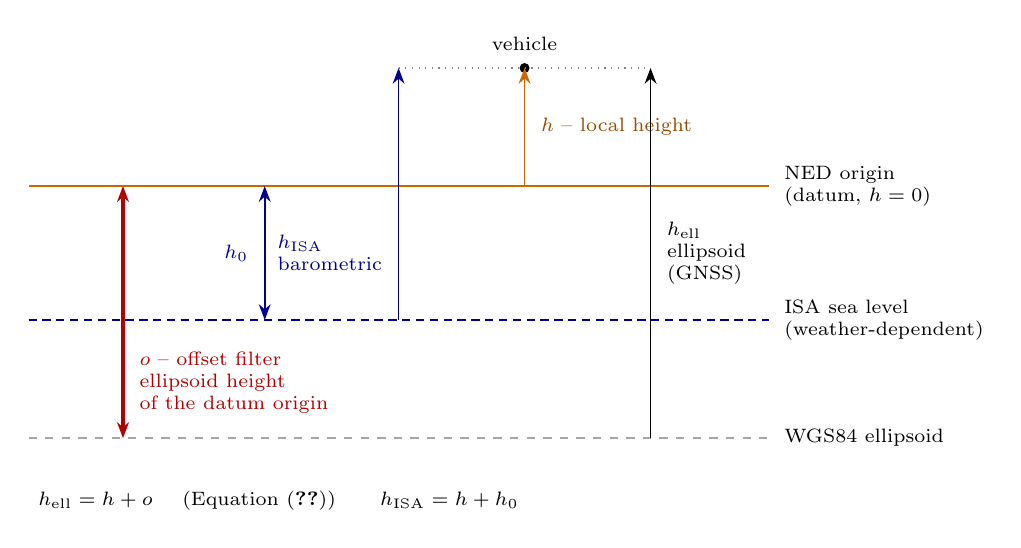
\begin{tikzpicture}[
  xscale=1.0, yscale=1.0,
  surf/.style={semithick},
  meas/.style={-{Stealth[length=2.0mm]}, semithick},
  both/.style={{Stealth[length=2.0mm]}-{Stealth[length=2.0mm]}, semithick},
  lab/.style={font=\scriptsize, align=left},
  tag/.style={font=\scriptsize, align=left, inner sep=1.5pt, fill=white}
]
  % --- reference surfaces (names in the right-hand column) --------------
  \draw[surf, dashed, gray!70] (0,0) -- (9.4,0)
    node[right, lab, black, xshift=2pt] {WGS84 ellipsoid};
  \draw[surf, blue!55!black, dash pattern=on 3pt off 2pt] (0,1.5) -- (9.4,1.5)
    node[right, lab, black, xshift=2pt] {ISA sea level\\{\scriptsize(weather-dependent)}};
  \draw[surf, orange!80!black] (0,3.2) -- (9.4,3.2)
    node[right, lab, black, xshift=2pt] {NED origin\\{\scriptsize(datum, $h = 0$)}};

  % --- vehicle ----------------------------------------------------------
  \fill[black] (6.3,4.7) circle (1.8pt);
  \node[lab, above] at (6.3,4.8) {vehicle};
  \draw[dotted, gray] (4.7,4.7) -- (7.9,4.7);

  % --- offset o: ellipsoid -> datum origin (band below ISA is free) -----
  \draw[both, very thick, red!70!black] (1.2,0) -- (1.2,3.2);
  \node[tag, anchor=west, text=red!70!black] at (1.35,0.7)
    {$o$ -- offset filter\\ellipsoid height\\of the datum origin};

  % --- baro anchor constant h0: ISA sea level -> datum origin -----------
  \draw[both, blue!55!black] (3.0,1.5) -- (3.0,3.2);
  \node[tag, anchor=east, text=blue!55!black] at (2.85,2.35) {$h_0$};

  % --- the three height systems ----------------------------------------
  \draw[meas, blue!55!black] (4.7,1.5) -- (4.7,4.7);
  \node[tag, anchor=east, text=blue!55!black] at (4.55,2.35)
    {$h_{\text{ISA}}$\\barometric};

  \draw[meas, orange!80!black] (6.3,3.2) -- (6.3,4.7);
  \node[tag, anchor=west, text=orange!60!black] at (6.45,3.95)
    {$h$ -- local height};

  \draw[meas, black] (7.9,0) -- (7.9,4.7);
  \node[tag, anchor=west] at (8.05,2.35) {$h_{\text{ell}}$\\ellipsoid\\{\scriptsize(GNSS)}};

  \node[lab, anchor=north west] at (0,-0.55)
    {$h_{\text{ell}} = h + o$ \quad(Equation~\eqref{eq:hell})\qquad
     $h_{\text{ISA}} = h + h_0$};
\end{tikzpicture}
\caption{The three height systems. The local height $h$ is measured from
the NED origin and is zero at the start point; the offset filter
estimates $o$, the ellipsoid height of that origin, which is what turns
a local height into an absolute one during a GNSS outage -- and, while
GNSS is up and \code{ins} runs on the barometric height source, what
measures how far \code{ins}'s own vertical datum has drifted away from
the ellipsoid, since nothing else re-ties it to GNSS
(\S\ref{sec:offsetfilter}). The barometric
ISA altitude is a third, non-absolute system, offset from the datum by
the anchor constant $h_0$. Note that the ISA sea level drifts against
the ellipsoid with the weather -- which is exactly why $o$ is modelled
as a random walk and not as a constant.}
\label{fig:heightsystems}
\end{figure}

\subsection{baro\_alt: 3-state baro/accelerometer filter}
\label{sec:baroalt}

Unlike \code{ins}/\code{ahrs} this is a plain (full-state) \emph{linear} Kalman
filter -- the model is linear, no error-state formulation is needed.
State vector:
\begin{equation}
  \vect{x} = \begin{bmatrix} h & v & a_b \end{bmatrix}\T ,
\end{equation}
height above datum $h$ (\si{\metre}, positive up), vertical velocity
$v$, and a slowly varying additive correction $a_b$ to the measured
vertical acceleration (absorbing accelerometer bias, attitude error and
gravity model error projected onto the vertical axis).

\paragraph{Prediction: accelerometer as control input.} Each IMU epoch
the body specific force is rotated to NED with the \emph{supplied}
attitude quaternion (from \code{ins} or an AHRS), gravity removed, sign
flipped to positive-up:
\begin{equation}
  a_{\text{up}} = -\left( \left[\Rbn\vect{f}^\bframe\right]_z
    + g \right).
\end{equation}
The state propagates with constant-acceleration kinematics:
\begin{equation}
  \vect{x}_{k+1} = \mat{\Phi}\,\vect{x}_k + \mat{B}\,a_{\text{up}},
  \qquad
  \mat{\Phi} = \begin{bmatrix}
    1 & \dt & \tfrac{1}{2}\dt^2 \\
    0 & 1 & \dt \\
    0 & 0 & 1
  \end{bmatrix},
  \qquad
  \mat{B} = \begin{bmatrix}
    \tfrac{1}{2}\dt^2 \\ \dt \\ 0
  \end{bmatrix},
\end{equation}
(note $\mat{\Phi}$ couples $a_b$ into $h, v$, so the effective
acceleration is $a_{\text{up}} + a_b$). Process noise in noise-input
form, $\mat{G} = [\vect{e}_1\;\;\vect{e}_2\;\;\vect{e}_3]$,
$\vect{Q} = [\sigma_h^2\dt,\;\sigma_a^2\dt,\; \sigma_b^2\dt]$, i.e.
\begin{equation}
  \mat{Q}_d = \diag(\sigma_h^2\,\dt,\ \sigma_a^2\,\dt,\ \sigma_b^2\,\dt).
\end{equation}
The accelerometer noise enters $v$'s own derivative directly (unit weight on
$\vect{e}_2$), \emph{not} through $\mat{B}$: without a noise column of its own,
$h$ would inherit $v$'s injected uncertainty only one step later, through
$\mat{\Phi}$'s $v\!\to\!h$ coupling. The exact continuous-discrete model for
this double integrator additionally places small
$Q_{hh}\!\sim\!\sigma_a^2\dt^3/3$ and $Q_{hv}\!\sim\!\sigma_a^2\dt^2/2$ terms
at every step, which the unit-weight-on-$v$-only $\mat{G}$ leaves at zero;
$\sigma_h$ (\code{h\_\allowbreak{}process\_\allowbreak{}noise\_\allowbreak{}m\_\allowbreak{}sqrthz}) is a deliberately small,
independently tunable stand-in for that omitted term -- a margin against
discretization/model mismatch, not a primary noise source.

$\sigma_h$, $\sigma_a$ (\code{acc\_\allowbreak{}noise\_\allowbreak{}mps2\_\allowbreak{}sqrthz}) and $\sigma_b$
(\code{acc\_\allowbreak{}bias\_\allowbreak{}drift\_\allowbreak{}mps2\_\allowbreak{}sqrthz}) are continuous-time spectral densities
(\si{\per\sqrt\hertz}) scaled by the actual $\dt$, so the injected variance per
second is IMU-rate-invariant; a fixed per-sample sigma would over- or
under-inject noise at other rates. The accelerometer is a control input,
\emph{not} a measurement: between barometer samples the filter dead-reckons on
it.

\paragraph{Barometer measurement.} Pressure is converted with the
International Standard Atmosphere:
\begin{equation}
  h_{\text{ISA}}(p) = 44330 \left( 1 -
    \left(\frac{p}{p_0}\right)^{1/5.255} \right)\ \si{\metre},
  \qquad p_0 = \SI{101325}{\pascal},
  \label{eq:isa}
\end{equation}
anchored at the init pressure sample: the anchor's ISA altitude
corresponds to the height $h_{\text{init}}$ above the caller's datum
(default 0 = ``height above start''), giving the datum zero point
$h_0 = h_{\text{ISA}}(p_{\text{anchor}}) - h_{\text{init}}$. Samples are
fused as the scalar $z = h_{\text{ISA}}(p) - h_0$ with
$\mat{H} = [1\;0\;0]$ through the same robust UDU update -- outliers
are downweighted (persistent absolute reference). Pressure plausibility
is enforced at the boundary (\SIrange{10}{120}{\kilo\pascal}).

\paragraph{Zero-velocity update.} A caller-triggered pseudo-measurement
(\code{baro\_\allowbreak{}alt\_\allowbreak{}zero\_\allowbreak{}velocity\_\allowbreak{}update}, e.g.\ driven by the same
stillness detector as \code{ins}'s own ZUPT/ZARU, \S\ref{sec:autozupt})
observes $v$ directly:
\begin{equation}
  z = 0, \qquad \mat{H} = \begin{bmatrix} 0 & 1 & 0 \end{bmatrix},
\end{equation}
fused through the same robust UDU update as the barometer (outliers
downweighted, not dropped). It is deliberately \emph{not} gated on the
filter's own $v$ estimate -- that estimate is exactly what is being
corrected, so gating on it would suppress the update precisely when the
accelerometer-only dead reckoning has drifted furthest and needs it
most. Beyond bounding $v$, the update also pulls on $a_b$ through the
$v/a_b$ covariance coupling built up by the prediction, so a standstill
corrects the acceleration bias even while the barometer is unavailable.

\paragraph{Precision restart watchdog.} Past a warm-up period after
init (\code{restart\_\allowbreak{}warmup\_\allowbreak{}sec}), the filter's own reported $h$ and
$v$ 1-sigma (from the UDU factors) are checked against
\code{restart\_\allowbreak{}h\_\allowbreak{}stddev\_\allowbreak{}m} / \code{restart\_\allowbreak{}v\_\allowbreak{}stddev\_\allowbreak{}mps}, if either
is exceeded the filter is marked uninitialized (the same fail-safe
mechanism as the general health check), e.g.\ after a long barometer
outage has left the accelerometer-only dead reckoning too uncertain to
trust. \code{nav\_\allowbreak{}suite} then re-bootstraps the vertical channel from
the live stream, a standalone caller must call \code{baro\_\allowbreak{}alt\_\allowbreak{}init}
again. Either threshold can be disabled individually (negative value),
or the whole watchdog turned off (\code{precision\_\allowbreak{}restart\_\allowbreak{}disable}).

\subsection{local\_gnss\_alt: 1-state offset filter}
\label{sec:offsetfilter}

A scalar random-walk Kalman filter estimates
\begin{equation}
  o = h_{\text{GNSS,ellipsoid}} - h_{\text{local}},
\end{equation}
the ellipsoid height of the datum origin (\S\ref{sec:heightsystems}).
The filter is deliberately \emph{agnostic} to where the local height
comes from: with the barometric source $o$ lumps the weather-dependent
pressure offset, the geoid undulation and the ISA model error, with an
external local height (e.g.\ a lighthouse system) it lumps the geoid
undulation and the datum's own height. Propagation
$\sigma_o^2 \mathrel{+}= \sigma_{\text{RW}}^2\,\dt$ (default
\SI{0.3}{\metre\per\sqrt\second}: slow enough to average pair noise,
fast enough for the ISA-model error, confidence decays during outages).
It is that term and not the weather that sizes the default. Weather
drift of metres per hour would be satisfied by an order of magnitude
less; the ISA error is instead a fraction of the height \emph{excursion}
-- a tenth of it is ordinary, the model assuming a sea-level temperature
the real atmosphere rarely has -- so a few hundred metres of terrain
climbed in a few minutes move $o$ by tens of metres in those minutes. A
random walk in \emph{time} can only bound a drift whose driver is
altitude, never model it, and the bound has to stay wide enough that the
chi-square screening below still reads such a drift as drift: too slow a
walk turns real, persistent drift into a stream of apparent outliers, and
the downweighting then holds $o$ back precisely when it has the most
catching up to do. Update with pair variance $R = \sigma_{\text{local}}^2
+ \sigma_{\text{GNSS}}^2$ and the same chi-square downweighting,
written out directly ($n{=}1$, no UDU needed):
\begin{equation}
  K = \frac{\sigma_o^2}{\sigma_o^2 + R}, \qquad
  o \leftarrow o + K\,\delta z, \qquad
  \sigma_o^2 \leftarrow (1 - K)\,\sigma_o^2 .
\end{equation}
Both stddevs are additionally derated by a configurable inflation factor
and the fusion is decimated to a configurable minimum interval, which
together keep a single pair from nudging the offset around.

\paragraph{Which local height to feed it with.} The suite feeds the filter from
the source that \emph{survives a GNSS outage} -- the barometer if it is running,
otherwise the \code{ins} local height -- and \emph{not} from the momentarily
most accurate one. While GNSS is up the \code{ins} local height is by far the
better estimate, but pairing it against GNSS would yield a drift-free $o$ that
is useless the moment it is needed, because the height it would then be added to
(the barometer's) carries a weather drift $o$ never learned to absorb. The same
reference evaluates Equation~\eqref{eq:hell}, so offset and height always refer
to one source.

\paragraph{Correcting the datum drift.} Under the barometric height source
\code{ins}'s absolute height is only as good as its vertical \emph{datum}, and
that datum is anchored once at bootstrap and never re-tied to GNSS
(REQ-NAV-055): the barometer's whole absolute error accumulates in it for the
rest of the run. Its height \emph{relative} to that datum stays excellent, so
the absolute accessor keeps \code{ins} and subtracts only how far $o$ has moved
since the datum was fixed. Two details make that safe. The anchor \emph{tracks}
$o$ while the filter is still converging and freezes when it settles -- a
snapshot taken mid-convergence books the remaining convergence as drift that
never happened, and being a constant, that error becomes a permanent bias. And
only the part of the drift exceeding one $\sigma$ of its own estimate is
applied, less that margin: \code{ins} is the better estimate whenever the datum
has \emph{not} moved, which is most missions most of the time, so replacing its
decimetre-grade height with $h + o$ outright would buy back tens of metres on a
long drive at the price of the offset filter's metre-grade noise on every
epoch everywhere else. When the fix is delayed, the local height is extrapolated to the
GNSS time of validity with the estimated climb rate.

\paragraph{Datum coupling.} The offset is tied to the datum and would have to
move with any datum relocation. Under the ``the datum never moves'' rule
(\S\ref{sec:datumarb}) that never arises: when the suite relocates the
\emph{ins} origin onto the (stationary) baro datum at a GNSS bootstrap, the
datum the offset refers to has \emph{not} moved, so the offset is left
untouched. Shifting it there would put a permanent $\Delta z$ error on every
absolute height.

% ==============================================================================
\section{Frame offsets and coordinate conversion}
\label{sec:frameoffsets}
% ==============================================================================

A vehicle rarely lives purely in the local $n$-frame: an indoor drone
must relate the Lighthouse system's frame to the suite's datum, and an
outdoor drone must turn WGS84 waypoints into the local frame its
controller flies in. The suite exposes both bridges as accessor pairs,
one per side.

\paragraph{Local-position frame (\S\ref{sec:datumarb}).} An external
local-positioning system reports in its own frame, whose origin is
arbitrary. The suite reconciles it by subtracting a constant offset
$\vect{o}_{\text{lp}}$ from every \code{local\_\allowbreak{}pos} before \code{ins}
consumes it, so \code{ins} always solves at $(0,0,h)$ relative to the
datum. $\vect{o}_{\text{lp}}$ is the external frame's coordinates of the
datum origin, exposed by \code{nav\_\allowbreak{}suite\_\allowbreak{}get\_\allowbreak{}local\_\allowbreak{}pos\_\allowbreak{}offset()}:
\begin{equation}
  \vect{p}_{\text{external}} = \vect{p}_{\text{local}} + \vect{o}_{\text{lp}},
  \qquad
  \vect{p}_{\text{local}} = \vect{p}_{\text{external}} - \vect{o}_{\text{lp}} .
\end{equation}
Its vertical component aligns to the barometric height that was already
established (which is what removes the height jump when the local system
comes online late), the horizontal component is the system's report at
first sample. The offset is tracked until \code{ins} locks the datum at
bootstrap, then frozen, and survives \code{ins} resets.

\paragraph{WGS84 (the GNSS side).} \code{nav\_\allowbreak{}suite\_\allowbreak{}local\_\allowbreak{}to\_\allowbreak{}wgs84()}
and its inverse \code{nav\_\allowbreak{}suite\_\allowbreak{}wgs84\_\allowbreak{}to\_\allowbreak{}local()} convert between a
local NED position (relative to the datum origin) and geodetic
lat/lon/ellipsoid-height, using the $n$-frame origin
$\vect{r}_{\text{origin}}^{\,e}$ and the $n\!\rightarrow\!e$ rotation:
\begin{equation}
  \vect{r}^{\,e} = \vect{r}_{\text{origin}}^{\,e}
    + \mat{R}^e_n\,\vect{p}_{\text{local}}^{\,n},
  \qquad
  \vect{p}_{\text{local}}^{\,n} = \mat{R}^n_e
    \left( \vect{r}^{\,e} - \vect{r}_{\text{origin}}^{\,e} \right),
\end{equation}
followed by the usual ECEF\,$\leftrightarrow$\,geodetic step. This is the
GNSS-side counterpart of the local-position offset: it turns the local
solution into WGS84 for telemetry, or WGS84 waypoints into the frame a
controller flies in.

Both WGS84 converters, like \code{nav\_\allowbreak{}suite\_\allowbreak{}get\_\allowbreak{}height\_\allowbreak{}ellipsoid}
(\S\ref{sec:heightsystems}), are available only once a real GNSS fix has
anchored the origin to WGS84 -- established by any usable fix, at
bootstrap or by fusion. Without it the origin is only the prescribed
init position (a rough indoor guess, or a lighthouse frame), so the
converters return false rather than emit a fictitious absolute
coordinate.

% ==============================================================================
\section{World Magnetic Model lookup}
% ==============================================================================
\label{sec:wmm}

\code{magnetic\_\allowbreak{}model} provides declination $D$, inclination $I$ and
total field strength $F$ for a position and decimal year, from
generated lookup tables (\code{wmm\_\allowbreak{}lut.h}, produced offline by
pygeomag-based generators) instead of an online spherical-harmonics
evaluation: fixed number of table lookups per call, no heap, bounded
time. Declination is stored on a fine grid and interpolated bilinearly
in space and linearly in time between the two model epochs, inclination
and field strength use a coarser grid, bilinear in space only (they
change slowly over a 5-year epoch). The NED reference vector is
assembled self-consistently as
\begin{equation}
  \vect{m}^\nframe = F
  \begin{bmatrix}
    \cos I \cos D \\ \cos I \sin D \\ \sin I
  \end{bmatrix}.
\end{equation}
Consumers: \code{ins\_\allowbreak{}set\_\allowbreak{}magnetic\_\allowbreak{}model\_\allowbreak{}from\_\allowbreak{}position()} builds
the full reference vector (so ins's vector fusion yaw is true-north)
and arms the field-strength gate,
\code{ahrs\_\allowbreak{}set\_\allowbreak{}position()} uses $D$ for the deterministic declination
step and $F$ for the opt-in gate. Like geodetic\_toolbox, the module
carries no filter policy -- ``is this measurement trustworthy'' is
decided in the filters.

% ==============================================================================
\section{Design decisions}
% ==============================================================================
\label{sec:decisions}

This section collects the load-bearing decisions and their rationale in
one place, the detailed context is in the sections above.

\begin{description}
  \item[UDU factorisation instead of a full covariance.]
    Single-precision hot path requires it, $\mat{P} \succeq 0$ by
    construction, roughly double effective precision
    (\S\ref{sec:udu}).
  \item[Error-state formulation (ins, ahrs).] The nominal state
    absorbs the nonlinear mechanisation, the Kalman filter sees small,
    nearly linear errors. Attitude errors stay far from singularities,
    the quaternion is corrected multiplicatively.
  \item[Downweight vs.\ skip per measurement class.] Persistent
    absolute references are downweighted (no deadlock on persistent
    offsets), high-rate local references are skipped (glitches are
    cheap to drop) -- \S\ref{sec:robust}.
  \item[Running mean instead of median for the ZARU average.] A median
    needs a buffer and selection ($O(k)$ memory, data-dependent work in
    the per-epoch path), the running mean is $O(1)$. WCET outranks
    statistical elegance here -- do not ``improve'' this.
  \item[Throttled covariance prediction.] Error dynamics are slow,
    predicting at IMU rate buys nothing but cycles
    (\S\ref{sec:predict}). Same reasoning throttles the AHRS covariance
    (20\,Hz) and its acc/mag fusion rates.
  \item[Vector vs.\ scalar magnetometer fusion.] ins fuses the field
    vector (with yaw-only Jacobian columns) -- \si{\micro\tesla} is
    contractual, enabling the magnitude gate by default and hard-iron
    bias estimation. The AHRS fuses a scalar heading -- unit-agnostic by
    design for direction-only sensors, so its magnitude gate is opt-in
    (\S\ref{sec:ahrs-mag}).
  \item[Hard-iron bias inside the filter, not outside.] Separability
    from yaw requires the yaw/bias cross-covariance, which only the
    filter maintains (\S\ref{sec:ins-mag}). Runtime-$n$ (15/18)
    instead of a second code path or a compile-time fork.
  \item[Re-acquisition keeps attitude and biases, but not the yaw
    \emph{prior}.] After a long outage position/velocity are gone but
    attitude/biases are the best-preserved states. Resetting them would
    require a static re-leveling phase the vehicle does not have at a
    tunnel exit. Yaw is the exception: with the state frozen, the
    platform's own rotation over the outage never entered it, so
    without an absolute heading its \emph{variance} goes back to
    ``unknown'' -- otherwise the heading correction ends up in the gyro
    $z$ bias (\S\ref{sec:readiness}).
  \item[History-anchored delayed fusion.] Residual at time of validity,
    covariance update on the current factors -- valid because the error
    state barely moves over a few hundred milliseconds
    (\S\ref{sec:delayed}).
  \item[Float states, double anchor.] Local float n-frame keeps the hot
    path fast on FPUs without double units, the double
    absolute anchor with incremental bookkeeping avoids the metre-scale
    quantisation of absolute float coordinates (\S\ref{sec:llh}).
  \item[Independent accelerometer noise defaults per filter.] The three
    ``accelerometer'' quantities are physically different measurements
    (raw VRW vs.\ leveling correction vs.\ attitude-projected vertical
    acceleration), sharing one constant regressed the vertical filter
    empirically (\S\ref{sec:defaults}). Gyro defaults \emph{are} shared
    -- same physical sensor in the suite.
  \item[Deterministic declination step.] Referencing to true north is a
    known rotation, so it is applied as an instantaneous re-frame of
    the nominal quaternion, not learned through the fusion (which would
    slew the heading over seconds and, transiently, disagree with the
    covariance).
  \item[Conservative defaults everywhere.] A zero/unset noise field
    never means ``no noise'' -- it means ``use a conservative
    consumer-MEMS placeholder''. An overconfident filter fails
    silently, an overly cautious one is just suboptimal.
  \item[Barometric height fused directly in \code{ins}, not switched in from
    \code{baro\_\allowbreak{}alt} on GNSS loss.] Two designs were considered: (a) keep
    \code{ins}'s height GNSS-only and let \code{nav\_\allowbreak{}suite} switch the reported
    height to \code{baro\_\allowbreak{}alt} whenever GNSS aiding drops, or (b) have
    \code{ins} itself fuse barometric height (\S\ref{sec:baro-height-meas}),
    replacing GNSS-derived height permanently once selected at bootstrap.

    (a) was rejected on two counts. A discrete switch between two
    independently-drifting estimates is a discontinuity by construction: no
    source stays a fixed distance from another over an arbitrary mission, so the
    step size is unbounded in general, not just in a corner case (on one real
    dataset the two disagreed by over ten metres after half an hour, entirely
    within continuous GNSS coverage). A hysteresis band only changes how rarely
    the jump happens. More fundamentally, splicing \code{ins}'s horizontal state
    onto \code{baro\_\allowbreak{}alt}'s independently-estimated vertical state discards the
    cross-covariance a single error-state filter maintains (an attitude error
    couples into all three position axes at once, \S\ref{sec:strapdown}), so the
    spliced vector is no longer a coherent minimum-variance estimate. (b) has
    neither problem: the height source is fixed once at bootstrap, so
    \code{ins}'s vertical state never switches mid-mission, and it stays inside
    \code{ins}'s own state and covariance.

    (b) does not remove the accessor-level handover:
    \code{nav\_\allowbreak{}suite\_\allowbreak{}get\_\allowbreak{}height} still falls back to \code{baro\_\allowbreak{}alt} outside
    \code{FULL} mode, because \code{ins} as a whole can be unavailable while a
    height is still wanted. What (b) changes is its \emph{character} -- both
    sides are then the same barometric quantity on one datum, so the step is the
    disagreement between two estimators of it rather than the gap between two
    height systems. That disagreement is cross-checked every epoch and warned
    about (REQ-SUITE-019).

    Two prices. \code{ins}'s height then depends on the barometer's absolute
    accuracy (weather/ISA model error) rather than GNSS's. That is the right
    trade for the height \emph{relative} to \code{ins}'s own vertical datum,
    where the barometer is the better instrument and GNSS's vertical accuracy
    is routinely the worse of the two. It is the wrong trade for the
    \emph{absolute} height, and not by a little: the datum is anchored once at
    bootstrap and never re-tied to GNSS, so the barometer's whole absolute
    error accumulates in it without bound. On a \SI{68}{\minute} drive over
    \SI{170}{\metre} of terrain that reached \SI{19}{\metre} RMS against a
    receiver whose own vertical spread at standstill measured
    \SI{0.08}{\metre} -- the premise that GNSS is the worse vertical source
    does not hold for a good receiver. The absolute accessor therefore
    \emph{corrects} \code{ins}'s height under this source by the offset
    filter's estimate of how far the datum has since drifted
    (\S\ref{sec:offsetfilter}), which is exactly the quantity that filter
    exists to track. It corrects rather than replaces: \code{ins} remains the
    better estimate whenever the datum has not moved. The relative accessor is
    unaffected.
    The second price, accepted: because the selection is never re-evaluated, a barometer
    failing mid-mission leaves the vertical channel without an absolute
    reference while GNSS keeps aiding the horizontal solution: re-evaluating per
    epoch would reintroduce exactly the discontinuity (a) was rejected for, so
    the case is mitigated rather than fixed -- the sample must be current at
    bootstrap, not merely present, and the ensuing aiding gap is reported
    explicitly (\S\ref{sec:auto-init}).
\end{description}

% ------------------------------------------------------------------------------
\section{Dataset configuration: \code{config.yaml}}
\label{sec:configyaml}
% ------------------------------------------------------------------------------

A dataset directory carries the neutral CSV streams
(\code{imu.csv}, \code{ref.csv}, and optionally \code{gnss.csv}, \code{mag.csv},
\code{baro.csv}, the column contract lives in \code{datasets/replay\_\allowbreak{}format.py})
plus one \code{config.yaml} that tells the harness \emph{how} to run the filter:
aiding source, initialisation mode, the sensor noise model, sensor calibration
and lever arms, aiding-quality gates, the (non-filter) scoring thresholds, and
optional per-stream CSV filename overrides.
Every key is optional except the IMU noise model (and \code{gnss:
pos\_\allowbreak{}stddev\_\allowbreak{}fallback\_\allowbreak{}m}/\code{vel\_\allowbreak{}stddev\_\allowbreak{}fallback\_\allowbreak{}mps} under
\code{aiding: ref}, see below), a value of $0$ (or an all-zero list) means
``use the built-in default / no-op'', never ``force zero''. An unknown key
is a hard error in both harnesses, naming the offending key: a silently
ignored key is indistinguishable from one that had no effect, so a typo
would otherwise produce a full run, a score and a plot computed with a
configuration nobody asked for.

``Known'' here means the \emph{schema}, not what a given harness happens to
consume. A dataset directory is read by more than the two replay harnesses --
\code{check\_\allowbreak{}simulated.py} owns \code{score: lim\_\allowbreak{}groves\_\allowbreak{}pos\_\allowbreak{}rms\_\allowbreak{}factor},
\code{crazyflie\_\allowbreak{}reader.py} owns the \code{origin:} and \code{crazyflie:}
sections -- so each harness also accepts, and ignores, the parts it does not
consume, from a list the two keep identical. Otherwise a dataset would have to
choose which of its tools it validates against, and deleting the offending key
would silently disarm the tool that does read it. A typo inside a section the
harness \emph{does} own remains an error, and a section earns the exemption
only once some tool actually reads it.

\medskip
\noindent The live receiver \code{tools/insrcv.c} reads the same file and is one
step more lenient: it implements a \emph{subset} of the schema, and a key it
does not consume is named on the console and then ignored instead of aborting
the run. Refusing to start a receiver over a \code{score:} section would be
useless, but a tuning value that silently has no effect misleads there as much
as in a replay -- so keys describing the replay harness itself (\code{score:},
\code{inputs:} and the \code{name}/\code{aiding}/\code{init} labels) pass
unremarked, and everything else the receiver does not implement is reported,
with the count repeated in its config summary line.

\medskip
\noindent A representative annotated example (keys not shown fall back to their
defaults):

\begin{lstlisting}[style=cfg]
name: my-dataset            # label for plots / the summary
aiding: gnss                # gnss | ref | none
init: auto                  # auto | ref
automotive_mode: 0          # 1: derive yaw from GNSS course-over-ground
chi2_disable: 0             # 1: disable outlier downweighting (diagnostics)
chi2_reject_alpha: 0.0      # 0 -> outlier gate, e.g. 0.05 -> 95% global
allow_unlimited_deadreckoning: 0  # 1: never expire the IMU-only coasting window
max_deadreckoning_sec: 0.0  # IMU-only coasting budget [s], 0 -> default 10 s
baro_height_disable: 0      # 1: never select the barometric height source,
                            #    keep GNSS position's vertical row. For a
                            #    gnss_pos stream that is not satellite GNSS
                            #    and is more accurate vertically than a
                            #    barometer (e.g. a Lighthouse/UWB rig), and
                            #    for a barometer whose static port does not
                            #    see ambient pressure: a sensor inside a car
                            #    cabin moves tens of metres with ventilation
                            #    and speed, far past any correction GNSS
                            #    could still apply, since the vertical row
                            #    is dropped for the whole run.
gyro_bias_window_sec: 3.0   # static window to seed the initial gyro bias
                            # (harness-only heuristic, no library default;
                            # 0 -> no seed at all)
auto_init_window_sec: 0.0   # IMU window ins levels over during auto-init [s]
                            # 0 -> default, raise it for a low IMU rate

imu:                        # sensor noise model (REQUIRED) + calibration
  gyr_psd:     3.0e-11      # gyro white noise PSD        [(rad/s)^2/Hz]
  acc_psd:     4.0e-06      # accel white noise PSD       [(m/s^2)^2/Hz]
  gyr_bias_rw: 1.4e-06      # gyro bias random walk       [rad/s/sqrt(s)]
  acc_bias_rw: 3.0e-04      # accel bias random walk      [m/s^2/sqrt(s)]
  # optional fixed calibration, corrected = M*(raw - bias):
  gyr_fixed_bias: [0,0,0]   # removed permanently, never estimated [rad/s]
  acc_fixed_bias: [0,0,0]                                        # [m/s^2]
  gyr_misalignment: [1,0,0, 0,1,0, 0,0,1]   # col-major 3x3 (0s->identity)
  acc_misalignment: [1,0,0, 0,1,0, 0,0,1]
  # extra process-noise margin on top of the acc/gyro-driven pos/vel/rpy
  # noise above, 0 -> default. The rpy default assumes a NON-RIGID mount,
  # where attitude model error dwarfs the gyro's random walk; a rigid mount
  # wants far less and sets it here.
  pos_pred_stddev_m_sqrts:   0.0  # [m/sqrt(s)]
  vel_pred_stddev_mps_sqrts: 0.0  # [m/s/sqrt(s)]
  rpy_pred_stddev_rad_sqrts: 0.0  # [rad/sqrt(s)]
  # Stillness: ONE set for the whole suite. It reaches ins, both AHRS
  # instances and (through them) baro_alt's vertical ZUPT -- the filters
  # implement it separately, they are not tuned separately.
  # Every field 0 -> the library's own default.
  #
  # pseudo-measurement stddev: how hard a detected standstill is trusted
  zero_vel_stddev_mps: 0.0        # [m/s]   (ins + baro_alt vertical ZUPT)
  zero_rot_stddev_deg: 0.0        # [deg/s] (ins + ARS/AHRS ZARU)
  # PRIMARY stillness criterion: per-axis RMS sample stddev of the raw
  # IMU over a short window (bias-invariant, hence primary)
  auto_zupt_static_gyr_stddev_deg:  0.0  # [deg/s]
  auto_zupt_static_acc_stddev_mps2: 0.0  # [m/s^2]
  # loose magnitude bounds beside it
  auto_zupt_static_gyr_deg:  0.0  # max |gyro| considered stationary [deg/s]
  auto_zupt_static_acc_mps2: 0.0  # max ||f| - g|                  [m/s^2]
  # velocity gate: applied only while a recent GNSS velocity exists that
  # is itself precise enough (no such fix -> the IMU decides alone; the
  # filter's own velocity state is never used, that would be circular)
  auto_zupt_max_vel_mps:        0.0  # max |GNSS velocity| to arm  [m/s]
  auto_zupt_max_vel_stddev_mps: 0.0  # max GNSS vel 1-sigma to trust it [m/s]
  # timing
  auto_zupt_dwell_sec:        0.0  # stillness required before a trigger [s]
  auto_zupt_min_interval_sec: 0.0  # min time between triggers          [s]
  # opt-outs
  auto_zupt_disable: 0  # 1 -> no stillness detection anywhere in the suite
  auto_zupt_velocity_blind_disable: 0  # 1 -> only the ARS/AHRS's own
                        # detector off (it cannot tell constant-velocity
                        # cruise from a standstill); ins keeps deciding

gnss:
  enable: 1                 # 0 -> the fixes are still read and counted,
                            # but none of them aids the filter
  leverarm_frd: [0,0,0]     # IMU->antenna lever arm, body FRD   [m]
  delay_ms: 0               # assumed fixed fix latency          [ms]
  max_horizontal_pos_stddev_m: 0.0    # fusion gate: ignore fixes worse than
  max_vertical_pos_stddev_m:   0.0    # this (per fix, see below), 0 -> ins.c's
  max_horizontal_vel_stddev_mps: 0.0  # own default, which is the accuracy CAP
  max_vertical_vel_stddev_mps:   0.0  # below (120 m / 60 m/s): by default no
                                       # fix is rejected for its reported
                                       # accuracy alone, it is capped and fused.
                                       # Set these below the caps for a hard gate.
  # 3D solution ENTRY gate (strict) + its dwell, 0 -> default:
  start_max_horizontal_pos_stddev_m: 0.0    # [m]
  start_max_vertical_pos_stddev_m:   0.0    # [m]
  start_max_horizontal_vel_stddev_mps: 0.0  # [m/s]
  start_max_vertical_vel_stddev_mps:   0.0  # [m/s]
  init_dwell_sec: 0.0       # how long the stream must stay entry-quality
  init_dwell_disable: 0     # 1: enter on the first good fix
  # 3D solution EXIT gate (loose) + its dwell, 0 -> ins.c's own default:
  stop_max_horizontal_pos_stddev_m: 0.0     # [m]
  stop_max_vertical_pos_stddev_m:   0.0     # [m]
  stop_max_horizontal_vel_stddev_mps: 0.0   # [m/s]
  stop_max_vertical_vel_stddev_mps:   0.0   # [m/s]
  stop_dwell_sec: 0.0       # bad-fix run before the 3D solution is left
  stop_disable: 0           # 1: never leave 3D on GNSS quality alone
  min_delay_ms: 0           # fusion rate limit: minimum time between two
                            # fixes the filter actually spends. A fix
                            # arriving sooner is skipped whole (both blocks)
                            # and counted in n_gnss_rate_limited; suspended
                            # while the coasting window is expired, so a
                            # tunnel exit is never paced. A GNSS error
                            # decorrelates over seconds, not over the fix
                            # interval, so fusing a 50 Hz stream at 50 Hz
                            # presents the same information ten times and
                            # collapses the covariance.
                            # 0 -> default (100 ms, 10 Hz), <0 -> no limit
  pos_decimation: 0         # fuse the position on every Nth epoch that
                            # offers BOTH a usable position and velocity,
                            # the velocity alone on the other N-1;
                            # 1 -> off, 0 -> ins.c's own default, which is
                            # OFF: min_delay_ms above covers the same
                            # over-fusing without withholding a block, and
                            # running both thins the position twice
  pos_stddev_fallback_m: [0,0]        # [hor,ver] used if reported cov is 0;
                                       # REQUIRED (no default) if aiding: ref,
                                       # where it is the ONLY noise the
                                       # truth-synthesized fix gets
  vel_stddev_fallback_mps: 0.0        # same, required if aiding: ref
  # The conditioning knobs below weight the FUSION only. The
  # fix-quality gates (max_*, start_max_*, stop_max_*, and the auto-ZUPT
  # accuracy gate) keep grading the stddev the receiver reported, so
  # downweighting a noisy receiver never silently stops the filter from
  # using it. Scale them freely against the gates. The pipeline runs
  #   envelope -> scale -> height scale -> floor -> cap -> manoeuvre term
  # and is described in REQ-NAV-038/041/071/072/073.
  acc_envelope_tau_sec: 0.0 # asymmetric tracking of the REPORTED accuracy:
                            # a rise takes effect at once, a fall only decays
                            # out with this time constant. A receiver's
                            # accuracy figure returns to nominal well before
                            # a re-acquired fix has actually settled.
                            # 0 -> default (5 s), <0 -> off
  pos_cov_scale: 0.0        # multiply reported pos stddev (0->1)
  pos_cov_scale_height: 0.0 # extra downweight of the pos HEIGHT axis (0->1)
  vel_cov_scale: 0.0
  pos_stddev_floor_hor_m: 0.0         # floor per-axis stddev (independently,
  pos_stddev_floor_ver_m: 0.0         # NOT correlation-preserving like
                                       # pos_cov_scale above: raises N/E/D
                                       # diagonal entries alone, so a
                                       # floored axis picks up the effect of
                                       # extra independent noise).
  vel_stddev_floor_hor_mps: 0.0       # Unlike the scales, 0 means "use ins.c's
  vel_stddev_floor_ver_mps: 0.0       # default", NOT "no floor". The defaults
                                       # (0.5/1.0 m, 0.3/0.5 m/s) describe a
                                       # single-frequency (L1) standalone
                                       # receiver, which is what an
                                       # unconfigured filter should assume: a
                                       # receiver claiming better than such a
                                       # solution can physically deliver is the
                                       # normal case, not the exception.
                                       #
                                       # A BETTER source must say so, or the
                                       # floors throw its precision away. Set
                                       # each floor to what that source really
                                       # delivers, e.g. for RTK fix:
                                       #   pos_stddev_floor_hor_m: 0.02
                                       #   pos_stddev_floor_ver_m: 0.03
                                       #   vel_stddev_floor_hor_mps: 0.03
                                       #   vel_stddev_floor_ver_mps: 0.05
                                       # A NEGATIVE value switches a floor off
                                       # entirely, i.e. trusts the reported
                                       # covariance unconditionally. Prefer
                                       # real numbers over -1: an RTK receiver
                                       # dropping to float or single still
                                       # reports optimistically, and a floor
                                       # sized for the fix mode is what keeps
                                       # that drop from being believed.
  pos_stddev_cap_hor_m: 0.0           # upper clamp, same 0 -> default /
  pos_stddev_cap_ver_m: 0.0           # <0 -> off convention (120 m, 60 m/s).
  vel_stddev_cap_hor_mps: 0.0         # Bounds what an unboundedly bad reported
  vel_stddev_cap_ver_mps: 0.0         # accuracy can do to the 32-bit hot path,
                                       # and is what lets max_* default to
                                       # "fuse everything". A cap below the
                                       # floor of the same axis group is raised
                                       # to that floor at init.
  vel_noise_acc_scale_hor: 0.0        # manoeuvre-dependent EXTRA velocity noise
  vel_noise_acc_scale_ver: 0.0        # in [m/s] per [m/s^2] of n-frame
                                       # ANTENNA acceleration (horizontal norm
                                       # on N/E, |Down| on D), added after the
                                       # cap. A Doppler velocity averages over
                                       # the receiver's measurement interval
                                       # while the state is instantaneous; under
                                       # acceleration the two differ by about
                                       # a*T/2, which the reported accuracy
                                       # cannot describe. The acceleration is
                                       # the antenna's, i.e. the body's plus the
                                       # centripetal term omega x (omega x l) of
                                       # the leverarm_b below (REQ-NAV-076), so
                                       # a platform turning about its own IMU
                                       # still pays for the arc its antenna
                                       # swings through. With no lever arm that
                                       # addition is exactly zero.
                                       # 0 -> default, <0 -> off. The defaults
                                       # (0.20 / 0.30) ARE that half-interval
                                       # for T = 400 ms, four times the rate
                                       # min_delay_ms paces fusion to (margin: T
                                       # belongs to the receiver's velocity
                                       # algorithm, not its output rate), plus a
                                       # margin on the vertical axis for its
                                       # one-sided satellite geometry. Fixed
                                       # constants: NOT derived from the
                                       # observed fix rate at runtime. At a
                                       # 45 deg lean that adds roughly 2 m/s,
                                       # more than six times the horizontal
                                       # velocity floor; at rest
                                       # it adds nothing, so the standstill
                                       # regime is untouched. Raise them for a
                                       # receiver whose velocity is
                                       # time-differenced carrier phase over a
                                       # long output interval (T is then the
                                       # full interval). Disable them for a
                                       # source with no measurement interval at
                                       # all, e.g. a pose tracker or a simulator.
  vel_noise_acc_window_sec: 0.0       # window the acceleration above is averaged
                                       # over: the SAME T the scales are half of.
                                       # The error priced is what averaging over
                                       # T does to a velocity, so the
                                       # acceleration over T is what sets it.
                                       # Without it a manoeuvre that just ended
                                       # goes unpriced on the fix that still
                                       # carries its error, and airframe
                                       # vibration is priced as if it were a
                                       # manoeuvre (measured: a zero-mean
                                       # 4 m/s^2 oscillation adds 4 (m/s)^2
                                       # instantaneous vs 0.01 windowed). The
                                       # VECTOR is averaged, so a zero-mean
                                       # swing cancels exactly. The rotation
                                       # half of the antenna acceleration uses
                                       # the same window but averages
                                       # omega*omega', which is quadratic and
                                       # therefore does NOT cancel for a
                                       # platform that turns back and forth.
                                       # 0 -> default (200 ms), <0 -> use the
                                       # instantaneous sample

init_stddev:                # initial-state 1-sigma (each 0 -> built-in default)
  pos_init_stddev_m: 0.0              # [m]
  vel_init_stddev_mps: 0.0            # [m/s]
  rpy_init_stddev_rad_deg:  0.0        # [deg]
  yaw_init_stddev_rad_deg:  0.0        # [deg] (0 -> rpy_init_stddev_rad_deg)
  acc_bias_init_stddev_mps2: 0.0      # [m/s^2]
  gyr_bias_init_stddev_rps_deg: 0.0   # [deg/s]

init_hint:                  # known initial roll/pitch/yaw for auto-init
                             # (init: auto only), roll/pitch used together,
                             # yaw independent, each 0 stddev -> no hint
  roll_deg: 0.0
  pitch_deg: 0.0
  rpy_stddev_deg: 0.0        # 0 -> no roll/pitch hint (usual: gravity levels it)
  yaw_deg: 0.0               # e.g. a known launch heading
  yaw_stddev_deg: 0.0        # 0 -> no yaw hint (usual: stays unknown until aiding)

mag:
  enable: 0                 # replay default (it opens mag.csv);
                             # tools/insrcv.c defaults to 1
  stddev_ut: 0.0            # heading-measurement noise [uT] (0 -> default)
  min_delay_ms: 0           # min. time between fusions (0 -> default,
                             # negative -> fuse every sample)
  wmm_year: 2025.0          # decimal year for the declination lookup
  estimate_bias: 0          # 18-state hard-iron bias
  fixed_bias: [0,0,0]       # hard-iron [uT],  misalignment: soft-iron 3x3
  misalignment: [1,0,0, 0,1,0, 0,0,1]

baro:
  enable: 0                 # Process barometer measurements
  stddev_m: 0.0             # Barometer measurement noise [m], 0 -> default
  acc_bias_rw: 0.0          # accel-bias drift  [m/s^2/sqrt(Hz)], 0 -> default
  acc_bias_init_mps2: 0.0   # INITIAL accel-bias stddev [m/s^2], 0 -> default
  acc_noise_mps2_sqrthz: 0.0 # accel-noise density [m/s^2/sqrt(Hz)]
  h_process_noise: 0.0      # direct height process noise [m/sqrt(Hz)], 0 -> default
  # local-height/GNSS-ellipsoid offset filter tuning (all 0 -> built-in
  # defaults). Raise local_gnss_rw_stddev_mps further for missions with
  # extreme altitude excursions (e.g. a soaring glider gaining kilometres
  # of altitude): the offset absorbs the ISA-model error, which grows with
  # the excursion and can outrun even the default, leaving the offset
  # permanently lagging.
  local_gnss_rw_stddev_mps: 0.0            # [m/sqrt(s)], 0 -> default 0.3
  local_gnss_chi2_threshold: 0.0           # 0 -> default chi2inv(0.95,1)
  local_gnss_min_update_interval_sec: 0.0  # [s], 0 -> default 10
  local_gnss_stddev_inflation_factor: 0.0  # 0 -> default 3
# Scalar ground speed from speed.csv (odometry, OBD-II). Uncertainty and
# delay are constants here, not per-sample columns.
speed:
  enable: 0                 # Process speed.csv
  scale: 0.0                # multiplies the reported speed, 0 -> 1.0
  stddev_mps: 0.0           # per-sample 1-sigma [m/s], 0 -> default
  stddev_rel: 0.0           # speed-proportional 1-sigma, 0 -> default
  min_speed_mps: 0.0        # skip below this FILTERED speed, 0 -> default
  delay_ms: 0               # how old a sample is at its timestamp

ahrs:                       # SHARED ARS/AHRS noise override (0 -> derived
                             # from imu: above), both sub-filters consume
                             # the same physical gyro/accelerometer
  gyr_noise_psd: 0.0        # [rad/s/sqrt(Hz)], 0 -> default
  gyr_bias_rw: 0.0          # [rad/s^2/sqrt(Hz)], 0 -> default
  acc_noise_mps2: 0.0       # [m/s^2], 0 -> default
  gyr_bias_init_stddev_rps_deg: 0.0  # [deg/s], 0 -> unchanged (the
                             # gyro_bias_window_sec seed's own stddev, or
                             # ahrs.c's default if that seed never ran)

score:                      # scoring/plots + regression gates ONLY (not filter)
  warmup_sec: 60.0
  ahrs: 1                   # also score the AHRS/ARS attitude filters
  leverarm_frd: [0,0,0]     # map the filter position onto the truth point
  min_epochs: 100
  lim_pos_rms_m: 2.0        # regression guard-rails (make simulated/datasets)
  lim_att_bias_deg: 0.1
  lim_yaw_std_deg: 0.2

inputs:                     # optional per-stream CSV filename overrides
  imu:  imu.csv             # each unset key -> the conventional <stream>.csv
  ref:  ref.csv
  gnss: gnss_f9p.csv        # e.g. swap only the receiver, keep the rest shared
  mag:  mag.csv
  baro: baro.csv
\end{lstlisting}

\paragraph{Top level.}
\begin{description}\setlength\itemsep{0pt}
  \item[\code{name}] \emph{string.} Dataset label used in plots and the summary.
  \item[\code{aiding}] \emph{default \code{gnss}.} Absolute-position source:
    \code{gnss} uses real per-epoch receiver covariance from \code{gnss.csv}
    (zero-diagonal entries replaced by the \code{gnss:} fallbacks), \code{ref}
    synthesises a fix from the ground truth with the \code{fix:} noise (not an
    independent error profile), \code{none} gives no position aiding at all --
    \code{ins} never initialises and only the ARS and \code{baro\_\allowbreak{}alt} filters
    run (\code{nav\_\allowbreak{}suite} \textsc{attitude-only} fallback).
  \item[\code{init}] \emph{default \code{auto}.} \code{auto}: \code{ins}
    auto-initialisation. \code{ref}: known initial state from the truth epoch
    aligned with the first IMU sample (a moving start is fine, e.g.\ an aircraft
    in cruise).
  \item[\code{automotive\_\allowbreak{}mode}] \emph{0/1, default 0.} Derive yaw from GNSS
    course-over-ground above a minimum speed, typically for wheeled,
    non-holonomic platforms without a magnetometer. \emph{Not} valid where
    course differs from heading at speed (aircraft in wind).
  \item[\code{automotive\_\allowbreak{}min\_\allowbreak{}speed\_\allowbreak{}mps}] \emph{m/s}
    Minimum ground speed for course-derived yaw.
  \item[\code{automotive\_\allowbreak{}min\_\allowbreak{}yaw\_\allowbreak{}stddev\_\allowbreak{}deg}] \emph{deg}
    Floor on the fused yaw stddev, raise (e.g.\ 15) to keep it a weak long-term
    anchor under wind drift.
  \item[\code{chi2\_\allowbreak{}disable}] \emph{0/1, default 0.} Disable chi\textsuperscript{2}
    outlier downweighting library-wide.
  \item[\code{chi2\_\allowbreak{}reject\_\allowbreak{}alpha}] \emph{default 0} Global
    significance level $\alpha$ of ins's chi\textsuperscript{2} downweight
    gate. Each absolute reference is fused scalar-row-wise (1 DOF), so a
    configured $\alpha$ sets one shared gate threshold
    $\chi^2_{\text{inv}}(1-\alpha, 1)$ for every channel (GNSS, magnetometer,
    local-position, yaw), evaluated by interpolating a fixed quantile table.
    $\alpha=0$ keeps ins.c's own single default (10.0, identical on all four
    channels -- no differing per-channel gates), a larger
    $\alpha$ (e.g.\ 0.05 $\to$ 3.84) is stricter, a smaller one more tolerant
    (e.g.\ 0.01 $\to$ 6.63).
    Ignored when \code{chi2\_\allowbreak{}disable} is set.
  \item[\code{gyro\_\allowbreak{}bias\_\allowbreak{}window\_\allowbreak{}sec}] \emph{s} Length of the
    initial static window averaged to seed the initial gyro-bias estimate.
  \item[\code{auto\_\allowbreak{}init\_\allowbreak{}window\_\allowbreak{}sec}] \emph{s, default 0 $\to$ default.}
    Length of the IMU window \code{ins}'s auto-initialisation levels over
    (median of the specific force, \S\ref{sec:auto-init}). Raise it for a low
    IMU rate so the window still contains enough samples.
  \item[\code{allow\_\allowbreak{}unlimited\_\allowbreak{}deadreckoning},
    \code{max\_\allowbreak{}deadreckoning\_\allowbreak{}sec}] \emph{0/1 and s, default 0 $\to$
    default.} IMU-only coasting budget before \code{is\_\allowbreak{}ready()} degrades
    (\S\ref{sec:readiness}); the flag makes the window never expire and
    then overrides the budget.
  \item[\code{baro\_\allowbreak{}height\_\allowbreak{}disable}] \emph{0/1, default 0.} Never select the
    barometric height source at bootstrap, keep the GNSS position's vertical
    row, even with a barometer present.
\end{description}

\paragraph{\code{imu:} --- noise model (required) and calibration.}
\begin{description}\setlength\itemsep{0pt}
  \item[\code{gyr\_\allowbreak{}psd}, \code{acc\_\allowbreak{}psd}] \emph{$(\mathrm{rad/s})^2$/Hz,
    $(\mathrm{m/s^2})^2$/Hz.} White-noise PSD (\code{replay.py} suggests values
    from a trial). \textbf{Required.}
  \item[\code{gyr\_\allowbreak{}bias\_\allowbreak{}rw}, \code{acc\_\allowbreak{}bias\_\allowbreak{}rw}] \emph{rad/s/$\sqrt{\mathrm s}$,
    m/s\textsuperscript{2}/$\sqrt{\mathrm s}$.} Bias random walk. Estimate from a
    long static log with \code{python/allan\_\allowbreak{}variance.py}. \textbf{Required.}
  \item[\code{gyr\_\allowbreak{}fixed\_\allowbreak{}bias}, \code{acc\_\allowbreak{}fixed\_\allowbreak{}bias}] \emph{3-list, rad/s and
    m/s\textsuperscript{2}, default 0.} Removed permanently ($\code{raw}-\code{bias}$),
    never estimated.
  \item[\code{gyr\_\allowbreak{}misalignment}, \code{acc\_\allowbreak{}misalignment}] \emph{9-list,
    column-major $3\times3$, all-zero $\to$ identity.} Scale/cross-coupling
    matrix $M$, $\code{corrected}=M(\code{raw}-\code{bias})$. Also feeds the
    parallel ARS/AHRS.

    Measured by \code{tools/inslib\_\allowbreak{}ubx\_\allowbreak{}imu\_\allowbreak{}calib.py} (or its window,
    \code{tools/inslib\_\allowbreak{}calib\_\allowbreak{}gui.py}) from a session of arbitrary static
    poses, no fixture involved. The same matrix carries the \emph{housing}
    alignment when one was captured: the unit is rested on a level surface,
    any tilt it reports is the IMU sitting crooked in the box, and the
    rotation that removes it is premultiplied onto $M$ for the
    accelerometer, the gyroscope and the magnetometer alike. One placement
    gives roll and pitch; a second on a face that is not parallel to the
    first also gives the yaw, which gravity on its own can never observe.
  \item[\code{pos\_\allowbreak{}pred\_\allowbreak{}stddev\_\allowbreak{}m\_\allowbreak{}sqrts}, \code{vel\_\allowbreak{}pred\_\allowbreak{}stddev\_\allowbreak{}mps\_\allowbreak{}sqrts},
    \code{rpy\_\allowbreak{}pred\_\allowbreak{}stddev\_\allowbreak{}rad\_\allowbreak{}sqrts}] \emph{m/$\sqrt{\mathrm s}$,
    m/s/$\sqrt{\mathrm s}$, rad/$\sqrt{\mathrm s}$} Extra process-noise margin added \emph{on top of} the
    physically-derived acc/gyro-driven pos/vel/rpy prediction noise, not
    instead of it.
\end{description}

\begin{figure}[htbp]
\centering
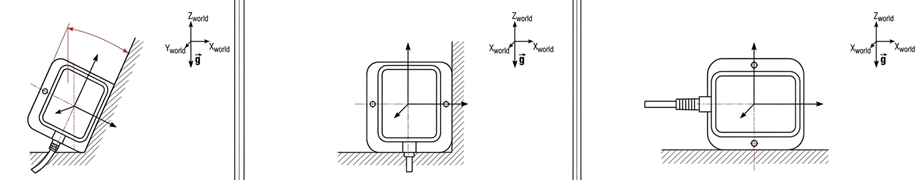
\includegraphics[width=0.92\textwidth]{figures/calibration.png}
\caption{Three of the static poses a calibration session collects: the unit
tilted against an edge, resting flat, and standing on its connector end,
each read against gravity in the world frame ($\vect{g}$, right of each
pose). Held-still orientations spanning enough of the sphere are what let
the fit separate bias, scale and misalignment without a turntable or
fixture -- see the coverage sphere below.}
\label{fig:calibposes}
\end{figure}

\noindent The same session also calibrates the magnetometer, when the board
streams one (\code{mag: fixed\_\allowbreak{}bias}/\code{misalignment} below): both are
fitted from one set of poses, not two separate sessions. Because of that,
\emph{the whole session -- not only the parts that look magnetometer-specific
-- has to happen away from ferrous material and active electronics}: a
steel desk, a nearby motor, or a metal-legged table all bias the field the
magnetometer fit reads, and nothing in the accelerometer/gyroscope channels
can detect that it happened. A genuinely magnetically clean surface is
harder to find than it sounds.

\begin{figure}[htbp]
\centering
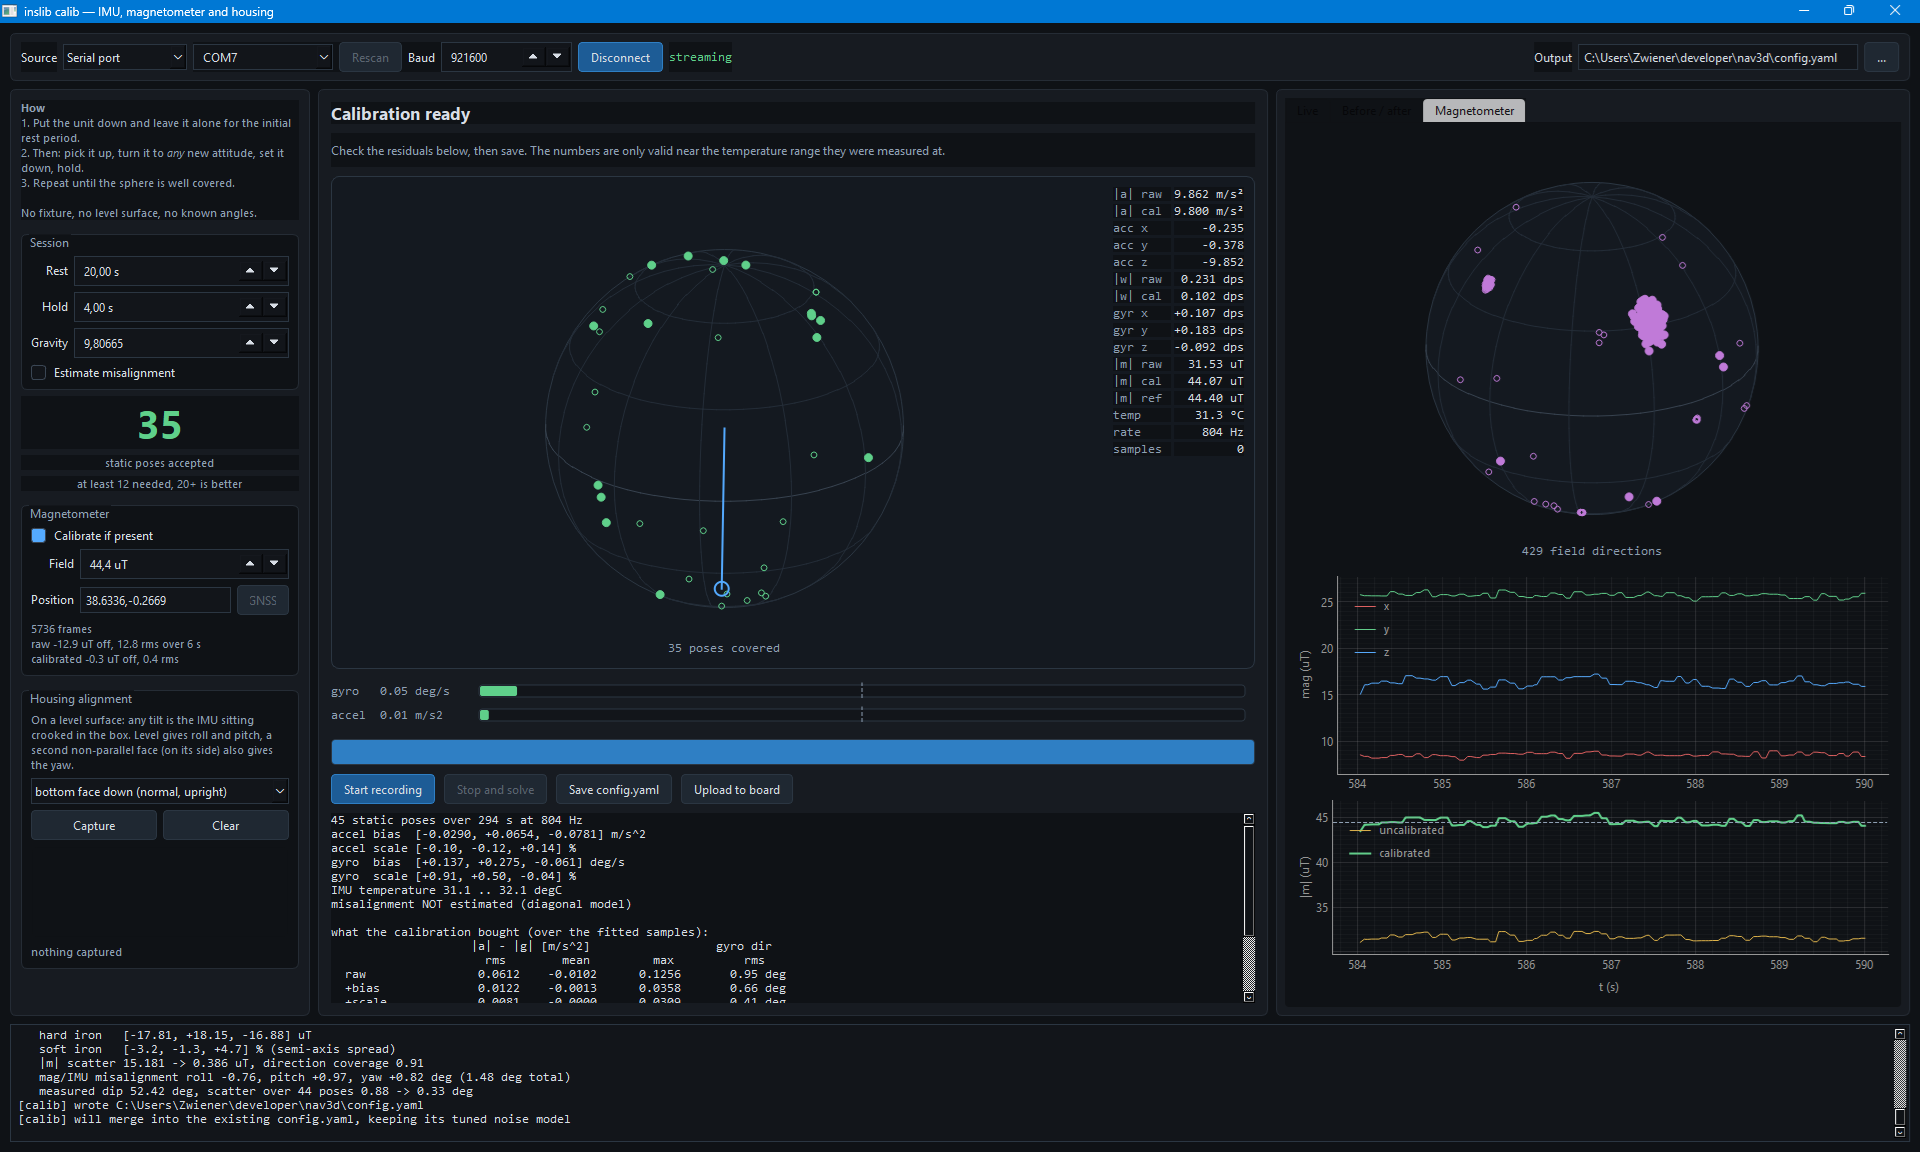
\includegraphics[width=0.92\textwidth]{figures/calib.png}
\caption{\code{tools/inslib\_\allowbreak{}calib\_\allowbreak{}gui.py}: the coverage sphere fills in as
static poses are accepted, the stillness meter says whether the unit
currently held down is calm enough to count, and the live traces show the
raw and calibrated readings side by side.}
\label{fig:calibgui}
\end{figure}

\paragraph{\code{imu:} --- stillness (all optional, $0 \to$ a default).}
One set for the whole suite: it configures
\code{ins}, both AHRS instances and \code{baro\_\allowbreak{}alt}'s vertical
zero-velocity update alike (\S\ref{sec:autozupt}). Neither harness
configures the ARS/AHRS gates separately any more.
\begin{description}\setlength\itemsep{0pt}
  \item[\code{zero\_\allowbreak{}vel\_\allowbreak{}stddev\_\allowbreak{}mps}, \code{zero\_\allowbreak{}rot\_\allowbreak{}stddev\_\allowbreak{}deg}]
    \emph{m/s, deg/s} Pseudo-measurement stddev: how hard a detected
    standstill is trusted once flagged. \code{zero\_\allowbreak{}vel\_\allowbreak{}stddev\_\allowbreak{}mps}
    also becomes \code{baro\_\allowbreak{}alt}'s vertical ZUPT stddev,
    \code{zero\_\allowbreak{}rot\_\allowbreak{}stddev\_\allowbreak{}deg} the ARS/AHRS zero-rotation stddev.
    These two are the one exception to ``$0 \to$ the library's own
    default'': both replay harnesses substitute their own
    0.05\,m/s and 0.1\,deg/s, the latter deliberately tighter than
    \code{ins}'s built-in 0.5\,deg/s, so a config that leaves them at 0
    keeps the historical harness tuning instead of silently loosening the
    rotation channel. Every remaining key below falls back to the
    library's own default.
  \item[\code{auto\_\allowbreak{}zupt\_\allowbreak{}static\_\allowbreak{}gyr\_\allowbreak{}stddev\_\allowbreak{}deg},
    \code{auto\_\allowbreak{}zupt\_\allowbreak{}static\_\allowbreak{}acc\_\allowbreak{}stddev\_\allowbreak{}mps2}] \emph{deg/s,
    m/s\textsuperscript{2}} The PRIMARY stillness criterion
    (\S\ref{sec:autozupt}): max per-axis RMS sample stddev of the raw
    gyro/accelerometer over a short window.
  \item[\code{auto\_\allowbreak{}zupt\_\allowbreak{}static\_\allowbreak{}gyr\_\allowbreak{}deg},
    \code{auto\_\allowbreak{}zupt\_\allowbreak{}static\_\allowbreak{}acc\_\allowbreak{}mps2}] \emph{deg/s,
    m/s\textsuperscript{2}} The loose magnitude bounds beside it: max
    $\|\vect{\omega}\|$ and max $\big|\|\vect{f}\| - g\big|$ still
    considered stationary.
  \item[\code{auto\_\allowbreak{}zupt\_\allowbreak{}max\_\allowbreak{}vel\_\allowbreak{}mps},
    \code{auto\_\allowbreak{}zupt\_\allowbreak{}max\_\allowbreak{}vel\_\allowbreak{}stddev\_\allowbreak{}mps}] \emph{m/s} The velocity
    gate: max $\|\vect{v}_{\text{GNSS}}\|$, and the accuracy (1-sigma,
    per axis) that GNSS velocity must itself report to count as
    evidence. Applied only while such a fix is recent enough; with
    none, only the IMU criteria decide. Not propagated to the ARS/AHRS,
    which have no velocity state.
  \item[\code{auto\_\allowbreak{}zupt\_\allowbreak{}dwell\_\allowbreak{}sec},
    \code{auto\_\allowbreak{}zupt\_\allowbreak{}min\_\allowbreak{}interval\_\allowbreak{}sec}] \emph{s} How long the
    platform must look still before a trigger, and how often triggers
    may repeat.
  \item[\code{auto\_\allowbreak{}zupt\_\allowbreak{}disable}] \emph{0/1, default 0.} Turn off
    every stillness source in the suite -- \code{ins}, both AHRS
    instances and, transitively, \code{baro\_\allowbreak{}alt}'s vertical ZUPT.
  \item[\code{auto\_\allowbreak{}zupt\_\allowbreak{}velocity\_\allowbreak{}blind\_\allowbreak{}disable}] \emph{0/1, default
    0.} Turn off only the ARS/AHRS's own velocity-blind detector
    (\S\ref{sec:autozupt}); \code{ins} keeps deciding for all of them.
\end{description}

\paragraph{\code{gnss:} --- aiding quality (all optional).}
\begin{description}\setlength\itemsep{0pt}
  \item[\code{leverarm\_\allowbreak{}frd}] \emph{3-list, m, body FRD, default 0.} IMU-to-antenna
    lever arm.
  \item[\code{delay\_\allowbreak{}ms}] \emph{ms, default 0.} Assumed fixed processing/telemetry
    latency, applied uniformly to every fix.
  \item[\code{max\_\{horizontal,vertical\}\_\{pos,vel\}\_stddev}]
    \emph{} Shutdown gates: a fix whose reported
    stddev exceeds the limit is ignored.
  \item[\code{pos\_\allowbreak{}stddev\_\allowbreak{}fallback\_\allowbreak{}m}, \code{vel\_\allowbreak{}stddev\_\allowbreak{}fallback\_\allowbreak{}mps}]
    \emph{[hor,ver] m and m/s, default 0.} Substituted for zero-diagonal reported
    covariance. \emph{REQUIRED (no default) under \code{aiding: ref}}: the
    reference-synthesized fix never has a reported covariance to begin
    with, so this is the only noise it gets -- \code{load\_\allowbreak{}config()} refuses
    to run without both.
  \item[\code{pos\_\allowbreak{}cov\_\allowbreak{}scale}, \code{vel\_\allowbreak{}cov\_\allowbreak{}scale}] \emph{default 0 $\to$ 1.}
    Multiply the reported stddev, for over-optimistic vendor covariance.
  \item[\code{pos\_\allowbreak{}cov\_\allowbreak{}scale\_\allowbreak{}height}] \emph{default 0 $\to$ 1.}
    Extra dedicated downweight of the GNSS position \emph{height} (Down) axis
    only, for receivers whose vertical solution is far worse than
    their horizontal one. Applied as the correlation-preserving congruence
    $\mat{S}\mat{Q}\mat{S}$ with $\mat{S}=\mathrm{diag}(1,1,s)$ (the N--D and
    E--D correlation coefficients are kept exactly), on top of
    \code{pos\_\allowbreak{}cov\_\allowbreak{}scale}, horizontal accuracy is untouched.
  \item[\code{\{pos,vel\}\_stddev\_floor\_...}] \emph{default 0.}
    Per-axis stddev floor, effective
    $\code{stddev}=\max(\code{scale}\cdot\code{reported},\code{floor})$.
\end{description}

\paragraph{\code{init\_\allowbreak{}stddev:} --- initial-state 1-sigma (REQ-VER-010).}
Each field mirrors \code{ins\_\allowbreak{}init\_\allowbreak{}t}, $0$ falls back to the built-in default.
Widen these when the ``known'' start is itself
only a GNSS-derived estimate, or the filter starts overconfident.
\begin{description}\setlength\itemsep{0pt}
  \item[\code{pos\_\allowbreak{}init\_\allowbreak{}stddev\_\allowbreak{}m}] m.
  \item[\code{vel\_\allowbreak{}init\_\allowbreak{}stddev\_\allowbreak{}mps}] m/s.
  \item[\code{rpy\_\allowbreak{}init\_\allowbreak{}stddev\_\allowbreak{}rad\_\allowbreak{}deg}] deg (roll/pitch, and yaw unless the next key is set).
  \item[\code{yaw\_\allowbreak{}init\_\allowbreak{}stddev\_\allowbreak{}rad\_\allowbreak{}deg}] deg, $0 \to$ \code{rpy\_\allowbreak{}init\_\allowbreak{}stddev\_\allowbreak{}rad\_\allowbreak{}deg}.
  \item[\code{acc\_\allowbreak{}bias\_\allowbreak{}init\_\allowbreak{}stddev\_\allowbreak{}mps2}] m/s\textsuperscript{2}.
  \item[\code{gyr\_\allowbreak{}bias\_\allowbreak{}init\_\allowbreak{}stddev\_\allowbreak{}rps\_\allowbreak{}deg}] deg/s.
\end{description}

\paragraph{\code{init\_\allowbreak{}hint:} --- known initial attitude for auto-init (optional, \code{init: auto} only).}
A static ``I just know it'' hint for \code{ins}'s auto-init bootstrap (e.g.\ a
known launch heading with no magnetometer/GNSS-course yaw aiding to derive it
from). Only used while neither the ARS nor the AHRS has initialised yet (a
continuously-running, converged heading takes priority once available) and only
until \code{ins} itself initialises.
\begin{description}\setlength\itemsep{0pt}
  \item[\code{roll\_\allowbreak{}deg}, \code{pitch\_\allowbreak{}deg}] \emph{deg, default 0.} Known initial
      roll/pitch, only used together (virtual measurement).
  \item[\code{rpy\_\allowbreak{}stddev\_\allowbreak{}deg}] \emph{deg, default 0 $\to$ no hint.} Shared
    roll/pitch 1-sigma for the virtual measurement. Usually left unset, since
    leveling is already observable from gravity.
  \item[\code{yaw\_\allowbreak{}deg}] \emph{deg, default 0.} Known initial yaw, independent
    of roll/pitch. A set yaw hint also seeds the yaw-free ARS's own initial
    heading, so \code{nav\_\allowbreak{}suite\_\allowbreak{}get\_\allowbreak{}rpy()} already reports it during the
    ATTITUDE\_ONLY window instead of the arbitrary 0 the ARS would otherwise
    start from. Roll/pitch are not seeded there (the ARS levels them from
    gravity on its first epoch).
  \item[\code{yaw\_\allowbreak{}stddev\_\allowbreak{}deg}] \emph{deg, default 0 $\to$ no hint.} Yaw stays
    unobservable until aiding arrives otherwise.
\end{description}

\paragraph{\code{ahrs:} --- SHARED ARS/AHRS noise override (all optional, default 0).}
The standalone ARS/AHRS attitude filters (\S\ref{sec:suite}) are
physically-separate filter instances from \code{ins} and are, by default, tuned from
the same \code{imu:} noise model above, \code{ahrs:} overrides that per
dataset instead, one call setting both sub-filters' template since they
consume the same physical gyro/accelerometer.
\begin{description}\setlength\itemsep{0pt}
  \item[\code{gyr\_\allowbreak{}noise\_\allowbreak{}psd}] \emph{rad/s/$\sqrt{\text{Hz}}$} Shared gyro noise density.
  \item[\code{gyr\_\allowbreak{}bias\_\allowbreak{}rw}] \emph{rad/s\textsuperscript{2}/$\sqrt{\text{Hz}}$,
    default 0 $\to$ default.} Shared gyro bias random walk density.
  \item[\code{acc\_\allowbreak{}noise\_\allowbreak{}mps2}] \emph{m/s\textsuperscript{2}, default 0 $\to$
    default.} Shared accelerometer noise stddev (leveling).
  \item[\code{gyr\_\allowbreak{}bias\_\allowbreak{}init\_\allowbreak{}stddev\_\allowbreak{}rps\_\allowbreak{}deg}] \emph{deg/s, default 0 $\to$
    unchanged.} Initial gyro-bias uncertainty for both sub-filters.
\end{description}

\paragraph{\code{mag:} and \code{baro:} --- optional sensors.}
\begin{description}\setlength\itemsep{0pt}
  \item[\code{mag: enable}] \emph{0/1, default 1 live, 0 offline.} Turn on
      magnetometer heading fusion. The two defaults differ because the key
      does two different things. Live (\code{tools/insrcv.c}) the
      \code{0x40/0x06} samples arrive over the wire regardless and the key
      gates the fusion alone (off, they stay decoded, counted and
      published), so a receiver with no magnetometer simply never fuses one
      and the default costs nothing --- as with the barometer. Offline
      (\code{tools/replay.c}, \code{python/replay.py}) the same key gates
      \emph{opening} \code{mag.csv} and a missing file is a hard error, so
      a dataset without a magnetometer stream must not have it on by
      default. The risk the live default accepts is an \emph{uncalibrated}
      sensor: hard iron is a bias, and no measurement noise removes the
      heading error it causes (\S\ref{sec:ins-mag}) --- only the
      calibration below does. It is acceptable because the failure is not
      silent: once a position is known, the field-strength gate
      downweights samples whose $|B|$ leaves the tolerance band and warns
      about a persistent deviation, which is what an uncorrected hard iron
      of any relevant size looks like. \code{insrcv} additionally says so
      at startup when the fusion is on and no calibration is configured.
  \item[\code{mag: stddev\_\allowbreak{}ut}] \emph{uT, default 0 $\to$ default.} Magnetometer
    measurement noise. The default is of the same order as the horizontal
    field itself, i.e.\ roughly a radian of heading noise per sample, see
    \S\ref{sec:ins-mag} for why weak is the right starting point. Lower it
    only for a sensor whose magnetic environment is known to be clean.
  \item[\code{mag: min\_\allowbreak{}delay\_\allowbreak{}ms}] \emph{ms, default 0 $\to$ default (1 Hz),
    negative $\to$ no rate limit.} Minimum time between two magnetometer
    fusions. The second half of the weighting decision above: the noise
    sets how far one sample may pull the heading, this sets how often it
    may (\S\ref{sec:ins-mag}). A source that is not a real magnetometer
    exposed to the platform (a synthesized or externally validated heading
    stream) is the case for switching the limit off.
  \item[\code{mag: wmm\_\allowbreak{}year}] \emph{decimal year.} Epoch for the World Magnetic
    Model declination lookup. Optional: without it the epoch comes from GPS
    time in the stream, failing that from the UTC date the receiver reports
    in NAV-PVT, and failing that from the host clock.
  \item[\code{mag: estimate\_\allowbreak{}bias}] \emph{0/1, default 0.} Run \code{ins} in its
    18-state mode estimating a hard-iron bias online.
    Observable only under rotation.
  \item[\code{mag: fixed\_\allowbreak{}bias}, \code{mag: misalignment}] \emph{3-list uT and
    9-list $3\times3$, defaults 0/identity.} Fixed hard-iron / soft-iron
    calibration, $\code{corrected}=M(\code{raw}-\code{bias})$.

    Measured alongside the IMU by the same tools when the board streams a
    magnetometer: turned through every attitude the sensor traces an
    ellipsoid, whose centre is the hard iron and whose shape is the soft
    iron. Fitting a sphere cannot see a rotation, so the fit is pinned to
    the symmetric square root and the leftover rotation is solved
    separately, from the fact that the angle between the local field and
    gravity cannot change with attitude. \code{misalignment} therefore also
    carries the mounting rotation of the magnetometer onto the IMU triad,
    without which a magnetometer a few degrees off its board contributes
    those same few degrees to the fused heading.
  \item[\code{baro: enable}] \emph{0/1, default 0 in the replay harnesses,
    1 in \code{tools/insrcv.c}.} Enable the \code{baro\_\allowbreak{}alt}
    vertical channel (needs static pressure measurements). The two defaults
    differ because the key does two different jobs: offline it gates
    \emph{opening} \code{baro.csv}, which a dataset without a barometer does
    not have, while the live receiver is handed pressure samples over the wire
    whether or not anyone asked for them -- there a default of 0 would take
    the vertical channel away from every session whose config predates the
    key. Set to 0 live, the samples are still decoded, counted, published to
    the telemetry stream and shown on the stats line (\code{baro-off=}), they
    simply aid nothing, the same A/B-comparable exclusion as
    \code{gnss: enable: 0}.
  \item[\code{baro: stddev\_\allowbreak{}m}] \emph{m, default 0 $\to$ default.} Barometric
    height noise.
  \item[\code{baro: acc\_\allowbreak{}bias\_\allowbreak{}rw}] \emph{m/s\textsuperscript{2}/$\sqrt{\text{Hz}}$,
    default 0 $\to$ default.} Continuous-time drift
    density $\sigma_b$ of the \code{baro\_\allowbreak{}alt} vertical-accelerometer bias state
    ($Q = \sigma_b^2\,\Delta t$), larger values let the estimated bias track
    faster. Note that this is a bias in the local navigation frame, not in the body frame.
  \item[\code{baro: acc\_\allowbreak{}bias\_\allowbreak{}init\_\allowbreak{}mps2}] \emph{m/s\textsuperscript{2},
    default 0 $\to$ default.} \code{baro\_\allowbreak{}alt}'s own INITIAL
    accel-bias uncertainty -- an initial condition, not a process-noise rate.
  \item[\code{baro: acc\_\allowbreak{}noise\_\allowbreak{}mps2\_\allowbreak{}sqrthz}] \emph{m/s\textsuperscript{2}/$\sqrt{\text{Hz}}$,
    default 0 $\to$ default.} \code{baro\_\allowbreak{}alt}'s own direct
    accelerometer-noise density, separate from other accelerometer noise settings as the measurement here
    is transformed into the navigation frame and can, for example, include attitude uncertainty.
  \item[\code{baro: h\_\allowbreak{}process\_\allowbreak{}noise}] \emph{m/$\sqrt{\text{Hz}}$, default
    0 $\to$ default.} Small direct process noise
    density $\sigma_h$ on \code{baro\_\allowbreak{}alt}'s height state
    (\code{h\_\allowbreak{}process\_\allowbreak{}noise\_\allowbreak{}m\_\allowbreak{}sqrthz}, \S\ref{sec:baroalt}) -- a
    safety margin against discretization/model mismatch, not a primary
    noise source.
\end{description}

\paragraph{\code{score:} --- evaluation only (never touches the filter).}
Used by the accuracy summary, the plots and the regression gates. \code{warmup\_\allowbreak{}sec}
[s, default 60] delays scoring after the first fix, \code{ahrs} [0/1] also scores
the attitude filters, \code{leverarm\_\allowbreak{}frd} [m] maps the filter position onto the
ground-truth point, \code{min\_\allowbreak{}epochs} sets the minimum scored-epoch count. The
\code{lim\_\allowbreak*} keys are the per-dataset
guard-rails that \code{make simulated}/\code{make datasets} trip on, they are
tuned regression thresholds, not accuracy claims, and each one at 0 is simply
not gated: \code{lim\_\allowbreak{}pos\_\allowbreak{}rms\_\allowbreak{}m} on horizontal position,
\code{lim\_\allowbreak{}att\_\allowbreak{}bias\_\allowbreak{}deg}/\code{lim\_\allowbreak{}att\_\allowbreak{}std\_\allowbreak{}deg} and
\code{lim\_\allowbreak{}yaw\_\allowbreak{}bias\_\allowbreak{}deg}/\code{lim\_\allowbreak{}yaw\_\allowbreak{}std\_\allowbreak{}deg} on attitude,
\code{lim\_baro\_\{rms,bias,max\}\_m} on the \code{baro\_\allowbreak{}alt} \emph{relative}
height, \code{lim\_ellipsoid\_\{rms,bias,max\}\_m} on the \emph{absolute}
ellipsoidal height the suite reports (\S\ref{sec:heightsystems}), and the
\code{lim\_\allowbreak{}ars\_\allowbreak*} attitude-fallback limits (\code{lim\_\allowbreak{}ars\_\allowbreak{}att\_\allowbreak{}bias\_\allowbreak{}deg},
\code{lim\_\allowbreak{}ars\_\allowbreak{}roll\_\allowbreak{}std\_\allowbreak{}deg}, \code{lim\_\allowbreak{}ars\_\allowbreak{}pitch\_\allowbreak{}std\_\allowbreak{}deg},
\code{lim\_\allowbreak{}ars\_\allowbreak{}yaw\_\allowbreak{}drift\_\allowbreak{}deg\_\allowbreak{}min}), which are only checked with
\code{ahrs: 1}. \code{attitude} [0/1, default 1] is the opt-out for a
dataset whose \code{ref.csv} carries no attitude truth: with it at 0 the
attitude columns are neither scored nor gated.

\paragraph{\code{inputs:} --- CSV filename overrides (optional).}
Per-stream keys \code{imu}, \code{ref}, \code{gnss}, \code{mag}, \code{baro},
each a filename resolved relative to the \code{config.yaml} directory. An unset
key keeps the conventional \code{<stream>.csv} name, so a dataset without an
\code{inputs:} block behaves exactly as before. This lets one stream be swapped
(e.g.\ \code{gnss: gnss\_\allowbreak{}f9p.csv}) while the remaining CSVs stay shared --- an
A/B comparison of two receivers or IMUs needs no directory duplication.

% ------------------------------------------------------------------------------
\subsection{\texorpdfstring{Parameter cross-reference: \code{config.yaml} $\leftrightarrow$ C API}{Parameter cross-reference: config.yaml vs. C API}}
\label{sec:configyaml-xref}
% ------------------------------------------------------------------------------

Table~\ref{tab:configyaml-xref} lists every \code{config.yaml} key next to the
C struct field or function call that ultimately consumes it, derived from
\code{tools/replay.c}'s \code{cfg\_\allowbreak{}set()} (the canonical, exhaustive mapping,
REQ-VER-025) -- \code{python/replay.py}'s \code{build\_\allowbreak{}config()} wires the
identical schema onto the same field names via ctypes. A key with no C
equivalent is consumed by the harness itself (dataset selection, CSV file
names, scoring) and never reaches the library. Fields written per epoch (into
\code{ins\_\allowbreak{}measurements\_\allowbreak{}t}, see \S\ref{sec:configyaml}) are marked
\emph{(per epoch)}; everything else is set once, before the replay loop
starts.

\begin{landscape}
\begin{center}
\small
\begin{longtable}{@{}p{6.5cm}p{16.5cm}@{}}
\caption{\code{config.yaml} key $\rightarrow$ C field / call.}
\label{tab:configyaml-xref}\\
\toprule
\textbf{\code{config.yaml} key} & \textbf{C field / call (header)} \\
\midrule
\endfirsthead
\multicolumn{2}{l}{\textit{(continued from previous page)}} \\
\toprule
\textbf{\code{config.yaml} key} & \textbf{C field / call (header)} \\
\midrule
\endhead
\midrule
\multicolumn{2}{r}{\textit{(continued on next page)}} \\
\endfoot
\bottomrule
\endlastfoot
\multicolumn{2}{l}{\textbf{Top level}} \\
\code{name}                & harness-only (dataset label) \\
\code{aiding}               & harness-only (selects \code{ins} aiding path) \\
\code{init}                 & harness-only (selects \code{ins\_\allowbreak{}options\_\allowbreak{}t.auto\_\allowbreak{}init}) \\
\code{automotive\_\allowbreak{}mode}     & \code{ins\_\allowbreak{}options\_\allowbreak{}t.automotive\_\allowbreak{}mode} (\code{ins.h}) \\
\code{automotive\_\allowbreak{}min\_\allowbreak{}speed\_\allowbreak{}mps} & \code{ins\_\allowbreak{}options\_\allowbreak{}t.automotive\_\allowbreak{}min\_\allowbreak{}speed\_\allowbreak{}mps} (\code{ins.h}) \\
\code{automotive\_\allowbreak{}min\_\allowbreak{}yaw\_\allowbreak{}stddev\_\allowbreak{}deg} & \code{ins\_\allowbreak{}options\_\allowbreak{}t.automotive\_\allowbreak{}min\_\allowbreak{}yaw\_\allowbreak{}stddev} (\code{ins.h}) \\
\code{chi2\_\allowbreak{}disable}        & \code{ins\_\allowbreak{}options\_\allowbreak{}t.chi2\_\allowbreak{}disable} (\code{ins.h}) \\
\code{chi2\_\allowbreak{}reject\_\allowbreak{}alpha}  & \code{ins\_\allowbreak{}options\_\allowbreak{}t.chi2\_\allowbreak{}reject\_\allowbreak{}alpha} (\code{ins.h}) \\
\code{allow\_\allowbreak{}unlimited\_\allowbreak{}deadreckoning} & \code{ins\_\allowbreak{}options\_\allowbreak{}t.allow\_\allowbreak{}unlimited\_\allowbreak{}deadreckoning} (\code{ins.h}) \\
\code{max\_\allowbreak{}deadreckoning\_\allowbreak{}sec} & \code{ins\_\allowbreak{}options\_\allowbreak{}t.max\_\allowbreak{}deadreckoning\_\allowbreak{}sec} (\code{ins.h}) \\
\code{baro\_\allowbreak{}height\_\allowbreak{}disable} & \code{ins\_\allowbreak{}options\_\allowbreak{}t.baro\_\allowbreak{}height\_\allowbreak{}disable} (\code{ins.h}) \\
\code{gyro\_\allowbreak{}bias\_\allowbreak{}window\_\allowbreak{}sec} & harness-only heuristic (seeds \code{ins\_\allowbreak{}init\_\allowbreak{}t.gyr\_\allowbreak{}bias\_\allowbreak{}init\_\allowbreak{}rps} / \code{ahrs\_\allowbreak{}config\_\allowbreak{}t.gyr\_\allowbreak{}bias\_\allowbreak{}init\_\allowbreak{}rps}) \\
\code{auto\_\allowbreak{}init\_\allowbreak{}window\_\allowbreak{}sec} & \code{ins\_\allowbreak{}options\_\allowbreak{}t.auto\_\allowbreak{}init\_\allowbreak{}window\_\allowbreak{}sec} (\code{ins.h}) \\
\addlinespace
\multicolumn{2}{l}{\textbf{\code{imu:} --- noise model and calibration}} \\
\code{gyr\_\allowbreak{}psd}             & \code{ins\_\allowbreak{}measurements\_\allowbreak{}t.gyr.Qll\_\allowbreak{}diag[\,]} \emph{(per epoch)} (\code{ins.h}) \\
\code{acc\_\allowbreak{}psd}             & \code{ins\_\allowbreak{}measurements\_\allowbreak{}t.acc.Qll\_\allowbreak{}diag[\,]} \emph{(per epoch)} (\code{ins.h}) \\
\code{gyr\_\allowbreak{}bias\_\allowbreak{}rw}        & \code{ins\_\allowbreak{}init\_\allowbreak{}t.gyr\_\allowbreak{}bias\_\allowbreak{}pred\_\allowbreak{}stddev\_\allowbreak{}rps\_\allowbreak{}sqrts} (\code{ins.h}); also the \code{ahrs:} default (\code{ahrs\_\allowbreak{}config\_\allowbreak{}t.gyr\_\allowbreak{}bias\_\allowbreak{}rw}, \code{ahrs.h}) \\
\code{acc\_\allowbreak{}bias\_\allowbreak{}rw}        & \code{ins\_\allowbreak{}init\_\allowbreak{}t.acc\_\allowbreak{}bias\_\allowbreak{}pred\_\allowbreak{}stddev\_\allowbreak{}mps2\_\allowbreak{}sqrts} (\code{ins.h}) \\
\code{gyr\_\allowbreak{}fixed\_\allowbreak{}bias}     & \code{ins\_\allowbreak{}options\_\allowbreak{}t.imu\_\allowbreak{}gyr\_\allowbreak{}fixed\_\allowbreak{}bias[3]} (\code{ins.h}) \\
\code{acc\_\allowbreak{}fixed\_\allowbreak{}bias}     & \code{ins\_\allowbreak{}options\_\allowbreak{}t.imu\_\allowbreak{}acc\_\allowbreak{}fixed\_\allowbreak{}bias[3]} (\code{ins.h}) \\
\code{gyr\_\allowbreak{}misalignment}    & \code{ins\_\allowbreak{}options\_\allowbreak{}t.imu\_\allowbreak{}gyr\_\allowbreak{}misalignment[9]} (\code{ins.h}) \\
\code{acc\_\allowbreak{}misalignment}    & \code{ins\_\allowbreak{}options\_\allowbreak{}t.imu\_\allowbreak{}acc\_\allowbreak{}misalignment[9]} (\code{ins.h}) \\
\code{pos\_\allowbreak{}pred\_\allowbreak{}stddev\_\allowbreak{}m\_\allowbreak{}sqrts} & \code{ins\_\allowbreak{}init\_\allowbreak{}t.pos\_\allowbreak{}pred\_\allowbreak{}stddev\_\allowbreak{}m\_\allowbreak{}sqrts} (\code{ins.h}) \\
\code{vel\_\allowbreak{}pred\_\allowbreak{}stddev\_\allowbreak{}mps\_\allowbreak{}sqrts} & \code{ins\_\allowbreak{}init\_\allowbreak{}t.vel\_\allowbreak{}pred\_\allowbreak{}stddev\_\allowbreak{}mps\_\allowbreak{}sqrts} (\code{ins.h}) \\
\code{rpy\_\allowbreak{}pred\_\allowbreak{}stddev\_\allowbreak{}rad\_\allowbreak{}sqrts} & \code{ins\_\allowbreak{}init\_\allowbreak{}t.rpy\_\allowbreak{}pred\_\allowbreak{}stddev\_\allowbreak{}rad\_\allowbreak{}sqrts} (\code{ins.h}) \\
\code{zero\_\allowbreak{}vel\_\allowbreak{}stddev\_\allowbreak{}mps} & \code{ins\_\allowbreak{}init\_\allowbreak{}t.zero\_\allowbreak{}vel\_\allowbreak{}stddev\_\allowbreak{}mps} (\code{ins.h}) \\
\code{zero\_\allowbreak{}rot\_\allowbreak{}stddev\_\allowbreak{}deg} & \code{ins\_\allowbreak{}init\_\allowbreak{}t.zero\_\allowbreak{}rot\_\allowbreak{}stddev\_\allowbreak{}rps} (\code{ins.h}) \\
\code{auto\_\allowbreak{}zupt\_\allowbreak{}static\_\allowbreak{}gyr\_\allowbreak{}stddev\_\allowbreak{}deg} & \code{ins\_\allowbreak{}options\_\allowbreak{}t.auto\_\allowbreak{}zupt\_\allowbreak{}static\_\allowbreak{}gyr\_\allowbreak{}stddev\_\allowbreak{}rps} (\code{ins.h}) \\
\code{auto\_\allowbreak{}zupt\_\allowbreak{}static\_\allowbreak{}acc\_\allowbreak{}stddev\_\allowbreak{}mps2} & \code{ins\_\allowbreak{}options\_\allowbreak{}t.auto\_\allowbreak{}zupt\_\allowbreak{}static\_\allowbreak{}acc\_\allowbreak{}stddev\_\allowbreak{}mps2} (\code{ins.h}) \\
\code{auto\_\allowbreak{}zupt\_\allowbreak{}static\_\allowbreak{}gyr\_\allowbreak{}deg} & \code{ins\_\allowbreak{}options\_\allowbreak{}t.auto\_\allowbreak{}zupt\_\allowbreak{}static\_\allowbreak{}gyr\_\allowbreak{}rps} (\code{ins.h}) \\
\code{auto\_\allowbreak{}zupt\_\allowbreak{}static\_\allowbreak{}acc\_\allowbreak{}mps2} & \code{ins\_\allowbreak{}options\_\allowbreak{}t.auto\_\allowbreak{}zupt\_\allowbreak{}static\_\allowbreak{}acc\_\allowbreak{}mps2} (\code{ins.h}) \\
\code{auto\_\allowbreak{}zupt\_\allowbreak{}max\_\allowbreak{}vel\_\allowbreak{}mps} & \code{ins\_\allowbreak{}options\_\allowbreak{}t.auto\_\allowbreak{}zupt\_\allowbreak{}max\_\allowbreak{}vel\_\allowbreak{}mps} (\code{ins.h}) \\
\code{auto\_\allowbreak{}zupt\_\allowbreak{}max\_\allowbreak{}vel\_\allowbreak{}stddev\_\allowbreak{}mps} & \code{ins\_\allowbreak{}options\_\allowbreak{}t.auto\_\allowbreak{}zupt\_\allowbreak{}max\_\allowbreak{}vel\_\allowbreak{}stddev\_\allowbreak{}mps} (\code{ins.h}) \\
\code{auto\_\allowbreak{}zupt\_\allowbreak{}dwell\_\allowbreak{}sec} & \code{ins\_\allowbreak{}options\_\allowbreak{}t.auto\_\allowbreak{}zupt\_\allowbreak{}dwell\_\allowbreak{}sec} (\code{ins.h}) \\
\code{auto\_\allowbreak{}zupt\_\allowbreak{}min\_\allowbreak{}interval\_\allowbreak{}sec} & \code{ins\_\allowbreak{}options\_\allowbreak{}t.auto\_\allowbreak{}zupt\_\allowbreak{}min\_\allowbreak{}interval\_\allowbreak{}sec} (\code{ins.h}) \\
\code{auto\_\allowbreak{}zupt\_\allowbreak{}disable} & \code{ins\_\allowbreak{}options\_\allowbreak{}t.auto\_\allowbreak{}zupt\_\allowbreak{}disable} (\code{ins.h}) \\
\code{auto\_\allowbreak{}zupt\_\allowbreak{}velocity\_\allowbreak{}blind\_\allowbreak{}disable} & \code{ins\_\allowbreak{}options\_\allowbreak{}t.auto\_\allowbreak{}zupt\_\allowbreak{}velocity\_\allowbreak{}blind\_\allowbreak{}disable} (\code{ins.h}) \\
\addlinespace
\multicolumn{2}{l}{\textbf{\code{gnss:} --- aiding quality}} \\
\code{leverarm\_\allowbreak{}frd}        & \code{ins\_\allowbreak{}measurements\_\allowbreak{}t.gnss\_\allowbreak{}leverarm\_\allowbreak{}b[3]} \emph{(per epoch)} (\code{ins.h}) \\
\code{delay\_\allowbreak{}ms}            & \code{ins\_\allowbreak{}measurements\_\allowbreak{}t.gnss\_\allowbreak{}delay\_\allowbreak{}ms} \emph{(per epoch)} (\code{ins.h}) \\
\code{pos\_\allowbreak{}stddev\_\allowbreak{}fallback\_\allowbreak{}m} & harness-only: fills a zero-diagonal \code{ins\_\allowbreak{}meas\_\allowbreak{}gnss\_\allowbreak{}pos\_\allowbreak{}t.Qll\_\allowbreak{}ned} \emph{(per epoch)} \\
\code{vel\_\allowbreak{}stddev\_\allowbreak{}fallback\_\allowbreak{}mps} & harness-only: fills a zero-diagonal \code{ins\_\allowbreak{}meas\_\allowbreak{}gnss\_\allowbreak{}vel\_\allowbreak{}t.Qll\_\allowbreak{}ned} \emph{(per epoch)} \\
\code{max\_\allowbreak{}horizontal\_\allowbreak{}pos\_\allowbreak{}stddev\_\allowbreak{}m} & \code{ins\_\allowbreak{}options\_\allowbreak{}t.gnss\_\allowbreak{}max\_\allowbreak{}horizontal\_\allowbreak{}pos\_\allowbreak{}stddev\_\allowbreak{}m} (\code{ins.h}) \\
\code{max\_\allowbreak{}vertical\_\allowbreak{}pos\_\allowbreak{}stddev\_\allowbreak{}m} & \code{ins\_\allowbreak{}options\_\allowbreak{}t.gnss\_\allowbreak{}max\_\allowbreak{}vertical\_\allowbreak{}pos\_\allowbreak{}stddev\_\allowbreak{}m} (\code{ins.h}) \\
\code{max\_\allowbreak{}horizontal\_\allowbreak{}vel\_\allowbreak{}stddev\_\allowbreak{}mps} & \code{ins\_\allowbreak{}options\_\allowbreak{}t.gnss\_\allowbreak{}max\_\allowbreak{}horizontal\_\allowbreak{}vel\_\allowbreak{}stddev\_\allowbreak{}mps} (\code{ins.h}) \\
\code{max\_\allowbreak{}vertical\_\allowbreak{}vel\_\allowbreak{}stddev\_\allowbreak{}mps} & \code{ins\_\allowbreak{}options\_\allowbreak{}t.gnss\_\allowbreak{}max\_\allowbreak{}vertical\_\allowbreak{}vel\_\allowbreak{}stddev\_\allowbreak{}mps} (\code{ins.h}) \\
\code{start\_\allowbreak{}max\_\allowbreak{}horizontal\_\allowbreak{}pos\_\allowbreak{}stddev\_\allowbreak{}m} & \code{ins\_\allowbreak{}options\_\allowbreak{}t.gnss\_\allowbreak{}start\_\allowbreak{}max\_\allowbreak{}horizontal\_\allowbreak{}pos\_\allowbreak{}stddev\_\allowbreak{}m} (\code{ins.h}) \\
\code{start\_\allowbreak{}max\_\allowbreak{}vertical\_\allowbreak{}pos\_\allowbreak{}stddev\_\allowbreak{}m} & \code{ins\_\allowbreak{}options\_\allowbreak{}t.gnss\_\allowbreak{}start\_\allowbreak{}max\_\allowbreak{}vertical\_\allowbreak{}pos\_\allowbreak{}stddev\_\allowbreak{}m} (\code{ins.h}) \\
\code{start\_\allowbreak{}max\_\allowbreak{}horizontal\_\allowbreak{}vel\_\allowbreak{}stddev\_\allowbreak{}mps} & \code{ins\_\allowbreak{}options\_\allowbreak{}t.gnss\_\allowbreak{}start\_\allowbreak{}max\_\allowbreak{}horizontal\_\allowbreak{}vel\_\allowbreak{}stddev\_\allowbreak{}mps} (\code{ins.h}) \\
\code{start\_\allowbreak{}max\_\allowbreak{}vertical\_\allowbreak{}vel\_\allowbreak{}stddev\_\allowbreak{}mps} & \code{ins\_\allowbreak{}options\_\allowbreak{}t.gnss\_\allowbreak{}start\_\allowbreak{}max\_\allowbreak{}vertical\_\allowbreak{}vel\_\allowbreak{}stddev\_\allowbreak{}mps} (\code{ins.h}) \\
\code{stop\_\allowbreak{}max\_\allowbreak{}horizontal\_\allowbreak{}pos\_\allowbreak{}stddev\_\allowbreak{}m} & \code{ins\_\allowbreak{}options\_\allowbreak{}t.gnss\_\allowbreak{}stop\_\allowbreak{}max\_\allowbreak{}horizontal\_\allowbreak{}pos\_\allowbreak{}stddev\_\allowbreak{}m} (\code{ins.h}) \\
\code{stop\_\allowbreak{}max\_\allowbreak{}vertical\_\allowbreak{}pos\_\allowbreak{}stddev\_\allowbreak{}m} & \code{ins\_\allowbreak{}options\_\allowbreak{}t.gnss\_\allowbreak{}stop\_\allowbreak{}max\_\allowbreak{}vertical\_\allowbreak{}pos\_\allowbreak{}stddev\_\allowbreak{}m} (\code{ins.h}) \\
\code{stop\_\allowbreak{}max\_\allowbreak{}horizontal\_\allowbreak{}vel\_\allowbreak{}stddev\_\allowbreak{}mps} & \code{ins\_\allowbreak{}options\_\allowbreak{}t.gnss\_\allowbreak{}stop\_\allowbreak{}max\_\allowbreak{}horizontal\_\allowbreak{}vel\_\allowbreak{}stddev\_\allowbreak{}mps} (\code{ins.h}) \\
\code{stop\_\allowbreak{}max\_\allowbreak{}vertical\_\allowbreak{}vel\_\allowbreak{}stddev\_\allowbreak{}mps} & \code{ins\_\allowbreak{}options\_\allowbreak{}t.gnss\_\allowbreak{}stop\_\allowbreak{}max\_\allowbreak{}vertical\_\allowbreak{}vel\_\allowbreak{}stddev\_\allowbreak{}mps} (\code{ins.h}) \\
\code{init\_\allowbreak{}dwell\_\allowbreak{}sec}     & \code{ins\_\allowbreak{}options\_\allowbreak{}t.gnss\_\allowbreak{}init\_\allowbreak{}dwell\_\allowbreak{}sec} (\code{ins.h}) \\
\code{init\_\allowbreak{}dwell\_\allowbreak{}disable} & \code{ins\_\allowbreak{}options\_\allowbreak{}t.gnss\_\allowbreak{}init\_\allowbreak{}dwell\_\allowbreak{}disable} (\code{ins.h}) \\
\code{stop\_\allowbreak{}dwell\_\allowbreak{}sec}     & \code{ins\_\allowbreak{}options\_\allowbreak{}t.gnss\_\allowbreak{}stop\_\allowbreak{}dwell\_\allowbreak{}sec} (\code{ins.h}) \\
\code{stop\_\allowbreak{}disable}        & \code{ins\_\allowbreak{}options\_\allowbreak{}t.gnss\_\allowbreak{}stop\_\allowbreak{}disable} (\code{ins.h}) \\
\code{pos\_\allowbreak{}decimation}      & \code{ins\_\allowbreak{}options\_\allowbreak{}t.gnss\_\allowbreak{}pos\_\allowbreak{}decimation} (\code{ins.h}) \\
\code{pos\_\allowbreak{}cov\_\allowbreak{}scale}      & \code{ins\_\allowbreak{}options\_\allowbreak{}t.gnss\_\allowbreak{}pos\_\allowbreak{}cov\_\allowbreak{}scale} (\code{ins.h}) \\
\code{pos\_\allowbreak{}cov\_\allowbreak{}scale\_\allowbreak{}height} & \code{ins\_\allowbreak{}options\_\allowbreak{}t.gnss\_\allowbreak{}pos\_\allowbreak{}cov\_\allowbreak{}scale\_\allowbreak{}height} (\code{ins.h}) \\
\code{vel\_\allowbreak{}cov\_\allowbreak{}scale}      & \code{ins\_\allowbreak{}options\_\allowbreak{}t.gnss\_\allowbreak{}vel\_\allowbreak{}cov\_\allowbreak{}scale} (\code{ins.h}) \\
\code{pos\_\allowbreak{}stddev\_\allowbreak{}floor\_\allowbreak{}hor\_\allowbreak{}m} & \code{ins\_\allowbreak{}options\_\allowbreak{}t.gnss\_\allowbreak{}pos\_\allowbreak{}stddev\_\allowbreak{}floor\_\allowbreak{}hor\_\allowbreak{}m} (\code{ins.h}) \\
\code{pos\_\allowbreak{}stddev\_\allowbreak{}floor\_\allowbreak{}ver\_\allowbreak{}m} & \code{ins\_\allowbreak{}options\_\allowbreak{}t.gnss\_\allowbreak{}pos\_\allowbreak{}stddev\_\allowbreak{}floor\_\allowbreak{}ver\_\allowbreak{}m} (\code{ins.h}) \\
\code{vel\_\allowbreak{}stddev\_\allowbreak{}floor\_\allowbreak{}hor\_\allowbreak{}mps} & \code{ins\_\allowbreak{}options\_\allowbreak{}t.gnss\_\allowbreak{}vel\_\allowbreak{}stddev\_\allowbreak{}floor\_\allowbreak{}hor\_\allowbreak{}mps} (\code{ins.h}) \\
\code{vel\_\allowbreak{}stddev\_\allowbreak{}floor\_\allowbreak{}ver\_\allowbreak{}mps} & \code{ins\_\allowbreak{}options\_\allowbreak{}t.gnss\_\allowbreak{}vel\_\allowbreak{}stddev\_\allowbreak{}floor\_\allowbreak{}ver\_\allowbreak{}mps} (\code{ins.h}) \\
\addlinespace
\multicolumn{2}{l}{\textbf{\code{init\_\allowbreak{}stddev:} --- initial-state 1-sigma}} \\
\code{pos\_\allowbreak{}init\_\allowbreak{}stddev\_\allowbreak{}m} & \code{ins\_\allowbreak{}init\_\allowbreak{}t.pos\_\allowbreak{}init\_\allowbreak{}stddev\_\allowbreak{}m} (\code{ins.h}) \\
\code{vel\_\allowbreak{}init\_\allowbreak{}stddev\_\allowbreak{}mps} & \code{ins\_\allowbreak{}init\_\allowbreak{}t.vel\_\allowbreak{}init\_\allowbreak{}stddev\_\allowbreak{}mps} (\code{ins.h}) \\
\code{rpy\_\allowbreak{}init\_\allowbreak{}stddev\_\allowbreak{}rad\_\allowbreak{}deg} & \code{ins\_\allowbreak{}init\_\allowbreak{}t.rpy\_\allowbreak{}init\_\allowbreak{}stddev\_\allowbreak{}rad[0..1]} (\code{ins.h}) \\
\code{yaw\_\allowbreak{}init\_\allowbreak{}stddev\_\allowbreak{}rad\_\allowbreak{}deg} & \code{ins\_\allowbreak{}init\_\allowbreak{}t.rpy\_\allowbreak{}init\_\allowbreak{}stddev\_\allowbreak{}rad[2]} (\code{ins.h}) \\
\code{acc\_\allowbreak{}bias\_\allowbreak{}init\_\allowbreak{}stddev\_\allowbreak{}mps2} & \code{ins\_\allowbreak{}init\_\allowbreak{}t.acc\_\allowbreak{}bias\_\allowbreak{}init\_\allowbreak{}stddev\_\allowbreak{}mps2} (\code{ins.h}) \\
\code{gyr\_\allowbreak{}bias\_\allowbreak{}init\_\allowbreak{}stddev\_\allowbreak{}rps\_\allowbreak{}deg} & \code{ins\_\allowbreak{}init\_\allowbreak{}t.gyr\_\allowbreak{}bias\_\allowbreak{}init\_\allowbreak{}stddev\_\allowbreak{}rps} (\code{ins.h}) \\
\addlinespace
\multicolumn{2}{l}{\textbf{\code{init\_\allowbreak{}hint:} --- auto-init attitude hint}} \\
\code{roll\_\allowbreak{}deg}, \code{pitch\_\allowbreak{}deg}, \code{rpy\_\allowbreak{}stddev\_\allowbreak{}deg}, \code{yaw\_\allowbreak{}deg}, \code{yaw\_\allowbreak{}stddev\_\allowbreak{}deg}
  & arguments of \code{nav\_\allowbreak{}suite\_\allowbreak{}set\_\allowbreak{}init\_\allowbreak{}att\_\allowbreak{}hint()} (\code{nav\_\allowbreak{}suite.h}) \\
\addlinespace
\multicolumn{2}{l}{\textbf{\code{mag:} --- magnetometer}} \\
\code{enable}               & harness-only (gates reading \code{mag.csv} / setting \code{ins\_\allowbreak{}measurements\_\allowbreak{}t.mag.is\_\allowbreak{}valid}) \\
\code{stddev\_\allowbreak{}ut}           & \code{ins\_\allowbreak{}measurements\_\allowbreak{}t.mag.Qll\_\allowbreak{}diag[\,]} \emph{(per epoch, squared)} (\code{ins.h}) \\
\code{min\_\allowbreak{}delay\_\allowbreak{}ms}       & \code{ins\_\allowbreak{}options\_\allowbreak{}t.magnetometer\_\allowbreak{}min\_\allowbreak{}delay\_\allowbreak{}ms} (\code{ins.h}) \\
\code{wmm\_\allowbreak{}year}            & argument of \code{ins\_\allowbreak{}set\_\allowbreak{}magnetic\_\allowbreak{}model\_\allowbreak{}from\_\allowbreak{}position()} (\code{ins.h}) and \code{ahrs\_\allowbreak{}set\_\allowbreak{}position()} (\code{ahrs.h}) \\
\code{estimate\_\allowbreak{}bias}       & \code{ins\_\allowbreak{}options\_\allowbreak{}t.estimate\_\allowbreak{}mag\_\allowbreak{}bias} (\code{ins.h}) \\
\code{fixed\_\allowbreak{}bias}          & \code{ins\_\allowbreak{}options\_\allowbreak{}t.mag\_\allowbreak{}fixed\_\allowbreak{}bias[3]} (\code{ins.h}) \\
\code{misalignment}         & \code{ins\_\allowbreak{}options\_\allowbreak{}t.mag\_\allowbreak{}misalignment[9]} (\code{ins.h}) \\
\addlinespace
\multicolumn{2}{l}{\textbf{\code{baro:} --- barometer}} \\
\code{enable}               & consumer-only (gates reading \code{baro.csv} resp. forwarding a received sample / setting \code{ins\_\allowbreak{}measurements\_\allowbreak{}t.baro.is\_\allowbreak{}valid}) \\
\code{stddev\_\allowbreak{}m}            & \code{ins\_\allowbreak{}measurements\_\allowbreak{}t.baro.stddev\_\allowbreak{}m} \emph{(per epoch)} (\code{ins.h}, also consumed by \code{baro\_\allowbreak{}alt} via \code{nav\_\allowbreak{}suite}) \\
\code{acc\_\allowbreak{}bias\_\allowbreak{}rw}        & \code{baro\_\allowbreak{}alt\_\allowbreak{}config\_\allowbreak{}t.acc\_\allowbreak{}bias\_\allowbreak{}drift\_\allowbreak{}mps2\_\allowbreak{}sqrthz} (\code{baro\_\allowbreak{}alt.h}) \\
\code{acc\_\allowbreak{}bias\_\allowbreak{}init\_\allowbreak{}mps2} & \code{baro\_\allowbreak{}alt\_\allowbreak{}config\_\allowbreak{}t.acc\_\allowbreak{}bias\_\allowbreak{}init\_\allowbreak{}stddev\_\allowbreak{}mps2} (\code{baro\_\allowbreak{}alt.h}) \\
\code{acc\_\allowbreak{}noise\_\allowbreak{}mps2\_\allowbreak{}sqrthz} & \code{baro\_\allowbreak{}alt\_\allowbreak{}config\_\allowbreak{}t.acc\_\allowbreak{}noise\_\allowbreak{}mps2\_\allowbreak{}sqrthz} (\code{baro\_\allowbreak{}alt.h}) \\
\code{h\_\allowbreak{}process\_\allowbreak{}noise}    & \code{baro\_\allowbreak{}alt\_\allowbreak{}config\_\allowbreak{}t.h\_\allowbreak{}process\_\allowbreak{}noise\_\allowbreak{}m\_\allowbreak{}sqrthz} (\code{baro\_\allowbreak{}alt.h}) \\
\addlinespace
\multicolumn{2}{l}{\textbf{\code{ahrs:} --- shared ARS/AHRS noise override}} \\
\code{gyr\_\allowbreak{}noise\_\allowbreak{}psd}      & \code{ahrs\_\allowbreak{}config\_\allowbreak{}t.gyr\_\allowbreak{}noise\_\allowbreak{}psd} (\code{ahrs.h}), applies to both \code{nav\_\allowbreak{}suite\_\allowbreak{}t.ars\_\allowbreak{}cfg} and \code{.ahrs\_\allowbreak{}cfg} \\
\code{gyr\_\allowbreak{}bias\_\allowbreak{}rw}        & \code{ahrs\_\allowbreak{}config\_\allowbreak{}t.gyr\_\allowbreak{}bias\_\allowbreak{}rw} (\code{ahrs.h}) \\
\code{acc\_\allowbreak{}noise\_\allowbreak{}mps2}     & \code{ahrs\_\allowbreak{}config\_\allowbreak{}t.acc\_\allowbreak{}noise\_\allowbreak{}mps2} (\code{ahrs.h}) \\
\code{gyr\_\allowbreak{}bias\_\allowbreak{}init\_\allowbreak{}stddev\_\allowbreak{}rps\_\allowbreak{}deg} & \code{ahrs\_\allowbreak{}config\_\allowbreak{}t.gyr\_\allowbreak{}bias\_\allowbreak{}init\_\allowbreak{}stddev\_\allowbreak{}rps[3]} (\code{ahrs.h}) \\
\addlinespace
\multicolumn{2}{l}{\textbf{\code{score:} and \code{inputs:} --- evaluation only}} \\
\code{score:*}              & harness-only (scoring, plots, regression gates -- never reaches the filter) \\
\code{inputs:*}             & harness-only (per-stream CSV filename overrides) \\
\end{longtable}
\end{center}
\end{landscape}

% ------------------------------------------------------------------------------
\subsection{Free-inertial mode (\code{free\_\allowbreak{}inertial\_\allowbreak{}start})}
\label{sec:freeinertial}
% ------------------------------------------------------------------------------

The 3D solution normally begins with a GNSS fix, because the strapdown
algorithm needs an absolute position to integrate away from. Free-inertial mode
allows it to manually supply the origin (instead of a GNSS receiver).

\medskip
\noindent\textbf{How it starts.} The declared position is offered to the filter
as a position measurement -- with the uncertainty the operator states, and
subject to the ordinary 3D entry gate -- and \emph{only until the filter has
bootstrapped from it}. Then the source goes silent. Once the
bootstrap has happened the filter runs on the IMU, the auto-ZUPTs
(section~\ref{sec:autozupt}) and the barometer, which is selected as the height
source at that bootstrap like in any other run (REQ-NAV-053).

\medskip
\noindent\textbf{What it deliberately switches off.} Enabling the mode is a
statement that coasting is the intent, not a fault, so the two mechanisms that
would otherwise end the run are taken out of the loop: the dead-reckoning
budget (\code{max\_\allowbreak{}deadreckoning\_\allowbreak{}sec}) and the 3D exit gate
(\code{gnss.stop\_\allowbreak{}disable}, REQ-NAV-052). Both exist to protect an
\emph{aided} solution from quietly degrading, and both would stop the filter
mid-experiment for doing exactly what it was asked to do. The 3D entry gate
stays in force and every fix is still judged on its own accuracy before it may
fuse: GNSS keeps its power to \emph{correct} the solution, it only loses its
power to \emph{end} it.

\medskip
\noindent\textbf{What it cannot deliver}. Heading is unobservable: without a
GNSS course and without a magnetometer nothing measures yaw, and at standstill
a MEMS gyroscope cannot find north either, its bias being orders of magnitude
above the earth rate. The dead-reckoned track therefore has a shape but no
absolute direction, and the yaw variance grows to ``unknown''.
Horizontal position drifts with nothing on board to correct it. The barometer
holds the vertical channel and the ZUPTs hold velocity and the IMU biases
whenever the platform stands still -- that is what makes such a run
informative, and it is also all of it.

\medskip
\noindent A typical configuration for an indoor inertial-sensor run, GNSS
excluded outright:

\begin{lstlisting}[style=cfg]
chi2_disable: 1             # outlier rejection off: expected at a standstill
                            # bootstrap and during ZUPT-only coasting

free_inertial_start:        # implemented by insrcv and both replay harnesses
  enable: 1                 # implies: no DR budget, no GNSS-quality exit
  lat_deg: 49.0             # where the platform starts, as well as known
  lon_deg: 8.4
  height_m: 118.0
  stddev_m: 0.05            # 1-sigma of that statement; must pass the
                            # 3D entry gate (gnss: start_max_horizontal_
                            # pos_stddev_m), so keep it at or below it

init_stddev:
  pos_init_stddev_m: 5.00
  vel_init_stddev_mps: 0.05
  yaw_init_stddev_rad_deg: 0.1

gnss:
  enable: 0                 # decode and publish, but aid nothing with it

baro:
  enable: 0                 # off here: this example is pure IMU-only
  acc_bias_init_mps2: 0.05
  stddev_m: 2.0

mag:
  enable: 0

imu:                        # the measured noise model of THIS sensor -
  gyr_psd: 5.0e-07          # in this mode nothing else constrains the
  acc_psd: 1.0e-05          # solution, so it is what the run is about
  gyr_bias_rw: 1.5e-05
  acc_bias_rw: 3.0e-04
  zero_vel_stddev_mps: 0.05 # the ZUPT is the only velocity measurement
  auto_zupt_dwell_sec: 0.1
  auto_zupt_static_gyr_stddev_deg: 0.35   # stillness thresholds against
  auto_zupt_static_acc_stddev_mps2: 0.45  # the sensor's own noise
  zero_rot_stddev_deg: 0.03 # left, so its stddev matters more than usual
\end{lstlisting}

\noindent\textbf{This example also excludes the barometer.} With
\code{baro: enable: 0} the vertical channel runs on the accelerometer and
the ZUPTs alone, drifting like the horizontal solution -- deliberately, to
demonstrate the pure-IMU extreme (no GNSS, no barometer, no magnetometer).
A barometer, where fused, would hold the vertical channel through the same
outage that leaves the horizontal solution to drift, exactly as described
above.

\noindent\textbf{Excluding GNSS outright.} \code{gnss: enable: 0} is a key of
its own, usable with or without the free-inertial start and implemented by all
three consumers. The fixes are still decoded, counted and (live) published to
the telemetry stream -- they simply aid nothing. That is deliberately different
from deleting \code{gnss.csv} or setting every gate to reject: the run stays
directly comparable against the same recording processed \emph{with} GNSS, one
key apart, which is what makes it an A/B rather than two different experiments.
On a real dataset the difference reads straight off the summary -- the same
3073 GNSS fixes are reported either way, while the filter goes from 2950 GNSS
fusions to none.

With GNSS excluded the magnetic model takes its anchor from the declared
position rather than from a fix, since declination and the reference field vary
on the scale of degrees of latitude and a hand-entered position is ample for
them. Its epoch comes from \code{mag: wmm\_\allowbreak{}year} if the config states one, from
GPS time when the stream carries a pulse, from the UTC date of the receiver's
own NAV-PVT when it does not, and otherwise from the host clock: a date is a
clock reading rather than a position measurement, so excluding GNSS as an
aiding source does not exclude it as a calendar, and no epoch at all would mean
no model at all, i.e. an AHRS referencing magnetic north without saying so. The
live receiver names the source it used in its log line, so a wrong date is
traceable rather than merely suspected.

\medskip
\noindent\textbf{The same run offline.} All three consumers implement the
section: the live receiver \code{tools/insrcv.c} and both replay harnesses
(\code{tools/replay.c}, \code{python/replay.py}). The same \code{config.yaml}
therefore produces the same start whether the data arrives over UDP or out of
\code{imu.csv}. The offer mechanism is identical in all three -- the declared
position at 2\,Hz until \code{ins} has bootstrapped from it, never in an epoch
that already carries a real fix, and the same two forced options -- which is
the point of a shared schema: a key that did something live and was quietly
ignored on replay would be precisely the silently ineffective setting this
chapter argues against.

Replayed this way a dataset needs no \code{gnss.csv} at all
(\code{aiding: none}), the declaration does the job the first fix would
otherwise do. For a stationary run the reference is worth having on top: if the
platform does not move, the truth is that it does not move, so a
\code{ref.csv} holding the constant start position turns the harness's scored
position error into a direct readout of the free-inertial drift.

\begin{lstlisting}[style=cfg]
name: indoor-free-inertial
aiding: none                # no gnss.csv, the declaration starts the filter
init: auto                  # bootstrap from it, exactly as the live path does
\end{lstlisting}

% ------------------------------------------------------------------------------
\subsection{Dataset CSV streams}
\label{sec:csvformat}
% ------------------------------------------------------------------------------

Alongside \code{config.yaml}, a dataset directory carries the sensor and
ground-truth streams as plain comma-separated files in one dataset-neutral
format (REQ-VER-003), written by the shared helpers in
\code{datasets/replay\_\allowbreak{}format.py} so the converters cannot drift apart and both
harnesses read the same bytes. Only \code{imu.csv} drives the filter,
\code{ref.csv} is the independent ground truth (used for scoring, for
\code{init: ref}, and to synthesise fixes under \code{aiding: ref}),
\code{gnss.csv}, \code{mag.csv} and \code{baro.csv} are consumed only when the
matching \code{aiding}/sensor option is on. The first line of each file is a
\code{\#} header, every column layout:

\begin{lstlisting}[basicstyle=\ttfamily\footnotesize,columns=fixed,keepspaces=true]
# imu.csv    (required, drives the filter)
  t_us, gx, gy, gz [rad/s], ax, ay, az [m/s^2]
  t_us, gx, gy, gz [rad/s], ax, ay, az [m/s^2], temp_c   (optional column)

# ref.csv    (required -- ground truth, ZYX roll/pitch/yaw)
  t_us, lat_deg, lon_deg, h_m, roll_deg, pitch_deg, yaw_deg, vn, ve, vd [m/s]

# gnss.csv   (aiding: gnss)   -- 20 fields, one fix per row
  t_us, lat_deg, lon_deg, h_m,
        cov_pos_ned nn,ne,nd,ee,ed,dd [m^2],
        vn, ve, vd [m/s],
        cov_vel_ned nn,ne,nd,ee,ed,dd [(m/s)^2],
        vel_ok

# mag.csv    (optional, mag: enable)
  t_us, mx, my, mz [uT]

# baro.csv   (optional, baro: enable)
  t_us, static_pressure [Pa]
\end{lstlisting}

\noindent Conventions shared by all streams:
\begin{description}\setlength\itemsep{0pt}
  \item[Timestamp \code{t\_\allowbreak{}us}] \code{int64} microseconds on one common clock,
    monotonically non-decreasing, the harness feeds each IMU epoch and then the
    most recent sample of every other stream at or before that time.
  \item[Frames] Body \textbf{FRD} (x forward, y right, z down) for IMU/mag,
    navigation \textbf{NED} for velocity and covariances, angles in degrees
    (\code{ref} attitude is Tait--Bryan ZYX roll/pitch/yaw). Position is
    geodetic \code{lat\_\allowbreak{}deg}/\code{lon\_\allowbreak{}deg} with ellipsoid height \code{h\_\allowbreak{}m}.
  \item[IMU] \code{gx..gz} are the body angular rate [rad/s], \code{ax..az} the
    specific force [m/s\textsuperscript{2}] (gravity included, so a level static
    unit reads $\approx(0,0,-g)$).
  \item[GNSS covariance] The 6 unique elements of the symmetric $3\times3$ NED
    covariance in order \code{nn,ne,nd,ee,ed,dd}. A \emph{zero diagonal} entry
    means ``unknown'' and is replaced at replay time by the \code{gnss:}
    fallback stddev (\S\ref{sec:configyaml}), \code{vel\_\allowbreak{}ok} (0/1) flags whether
    the velocity data is usable.
  \item[Header/comment lines] Any line beginning with \code{\#} is skipped, so
    the header row is informational. Rows with fewer than the required number of
    columns are ignored.
\end{description}

% ------------------------------------------------------------------------------
\subsection{\code{replay.py} analysis options (command line)}
\label{sec:replaycli}
% ------------------------------------------------------------------------------

The \emph{filter} behaviour is fixed by \code{config.yaml}
(\S\ref{sec:configyaml}), the Python harness \code{python/replay.py} adds a few
command-line flags that only affect \emph{analysis and output}, never the
estimate itself. \code{python/replay.py -{}-help} is authoritative, the flags
that change what is evaluated or reported are:

\begin{description}
  \item[\code{-{}-eval-start SEC}, \code{-{}-eval-end SEC}] Restrict the
    ground-truth error evaluation to a trial-time window (seconds from the first
    IMU sample, the same origin as the printed \code{t=\ldots} times). The
    filter still runs over the \emph{whole} trial -- so it stays converged --
    only the scored attitude/position error statistics and the
    \code{-{}-summary-json} output are limited to the window. The sensor
    data-quality checks (standstill accuracy, IMU noise) still use the full
    trial. Useful to exclude a bad startup segment or focus on one leg. Either
    bound may be given alone, the active window is echoed in the
    ``\code{ins vs ground truth}'' header.
  \item[\code{-{}-estimate-gnss-delay}] Force the GNSS-delay cross-correlation
    estimate on even outside the auto-detected case (\code{aiding: gnss} with
    usable velocity plus a barometer already runs it automatically, REQ-VER-009).
    Prints the estimated delay, its correlation quality, and -- when the
    correlation is trustworthy -- an actionable hint to set config
    \code{gnss: delay\_\allowbreak{}ms} (\S\ref{sec:configyaml}) to that value, the same
    number and hint appear on the GNSS-delay page of the \code{-{}-plot} PDF.
    The estimate is \emph{relative to} \code{baro\_\allowbreak{}alt}'s own (not necessarily
    zero) group delay.
  \item[\code{-{}-summary-json PATH}] Write the end-of-run accuracy summary
    (scored-epoch count, position RMS and maximum, roll/pitch/yaw error
    mean/std/max, warmup and evaluation window) as machine-readable JSON.
    Consumed by the simulated-dataset regression harness
    (\code{datasets/check\_\allowbreak{}simulated.py}, REQ-VER-016). It carries no pass/fail
        gates of its own (this stays a pure analysis tool).
  \item[\code{-{}-plot}, \code{-{}-plot-out PATH}] Render the multi-page
    diagnostic figures (state history, error, bias,
    ARS/AHRS, \code{baro\_\allowbreak{}alt}, altitude, GNSS delay, sensor rate, outliers)
    interactively or, with \code{-{}-plot-out}, as a single PDF (implies
    \code{-{}-plot}).
  \item[\code{-{}-plot-hz HZ}, \code{-{}-plot-track-hz HZ}] Sampling rates of
    the two \code{-{}-plot} recorders. \code{-{}-plot-hz} drives the state
    history behind every time-series page (roughly 60 fields per tick).
    \code{-{}-plot-track-hz} drives the North-East map page alone, which
    stores nothing but the North/East pair and therefore runs an order of
    magnitude faster: on a track spanning a few metres, every sample the
    recorder misses shows up as a chord across the real path. The map page
    then thins its vertices geometrically, to a tolerance relative to the
    extent of the track rather than to a fixed sample count, so the drawn
    resolution follows the scale of the view (millimetres on a 2\,m track,
    metres on a 10\,km one) at nearly constant page size. \code{0} makes
    the map reuse the \code{-{}-plot-hz} samples.
\end{description}


% ==============================================================================
\section{Verification environment (overview)}
% ==============================================================================

For completeness -- the process itself is documented in
\code{requirements/README.md}:

\begin{itemize}
  \item \textbf{Requirements database} (\code{requirements/req\_\allowbreak*.md}):
    aerospace-style, machine-checked by \code{make reqs} (unique IDs,
    status, parent links, and resolution of every \code{Test:}
    reference against the actual test code, \code{@satisfies} trace
    tags in \code{src/}).
  \item \textbf{Synthetic tests} (\code{make test}): plain-C scenario
    tests for all filters, no framework, non-zero exit on failure.
  \item \textbf{Real-data replays} (\code{make datasets}): 
    dataset processing harness (\code{tools/replay.c}, mirrored by
    \code{python/replay.py}) replays datasets for verification.
  \item \textbf{Static analysis} (\code{make cppcheck}, \code{make
    clang-tidy}): complements the compiler warnings (\code{-Wall -Wextra} plus
    a wider set) with two independent tools over the production sources.
    \code{make check-all} runs every gate above (plus \code{make coverage}
    and a \code{make doxygen} pass that treats any undocumented function or
    parameter as a failure) independently and prints a pass/fail summary,
    for pre-push or CI use. \item \textbf{Coverage} (\code{make coverage}): lcov HTML report
    including branch (and, with gcc $\ge$ 14.2, MC/DC) coverage.
\end{itemize}

% ==============================================================================
\begin{thebibliography}{9}

\bibitem{wendel2011}
J.~Wendel,
\emph{Integrierte Navigationssysteme: Sensordatenfusion, GPS und
Inertiale Navigation}, 2nd ed., Oldenbourg, 2011.

\bibitem{titterton2004}
D.~H.~Titterton and J.~L.~Weston,
\emph{Strapdown Inertial Navigation Technology}, 2nd ed., IET, 2004.

\bibitem{bierman1977}
G.~J.~Bierman,
\emph{Factorization Methods for Discrete Sequential Estimation},
Academic Press, 1977.

\bibitem{grewal2015}
M.~S.~Grewal and A.~P.~Andrews,
\emph{Kalman Filtering: Theory and Practice Using MATLAB}, 4th ed.,
Wiley, 2015.

\bibitem{chang2014}
G.~Chang,
``Robust Kalman filtering based on Mahalanobis distance as outlier
judging criterion,''
\emph{Journal of Geodesy}, vol.~88, no.~4, pp.~391--401, 2014.

\bibitem{groves2013}
P.~D.~Groves,
\emph{Principles of GNSS, Inertial, and Multisensor Integrated
Navigation Systems}, 2nd ed., Artech House, 2013.

\bibitem{carpenter2018}
J.~R.~Carpenter and C.~N.~D'Souza,
\emph{Navigation Filter Best Practices}, NASA/TP-2018-219822,
NF1676L-29886, 2018.
\url{https://ntrs.nasa.gov/api/citations/20180003657/downloads/20180003657.pdf}

\end{thebibliography}

\end{document}
